%% Preamble (document settings and packages)
\documentclass[a4paper,12pt,openright,oneside]{book}

% Enables Portuguese Brasil
\usepackage[portuguese]{babel}

% Enables code listing
\usepackage{listings}

% Enables file importing
\usepackage{import}

% Enables landscape orientation for certain pages
\usepackage{lscape}

%--------------------------------------

\usepackage{xcolor}

%--------------------------------------

\usepackage[T1]{fontenc}
\usepackage[utf8]{inputenc}

\usepackage[figuresright]{rotating}
\usepackage{amsthm}
\usepackage{graphics}
\usepackage{amssymb}
\usepackage{graphicx}
\usepackage{fancybox}
\usepackage{amsmath}
\usepackage{picinpar}
\usepackage{colortbl}
\usepackage{wasysym}
\usepackage{txfonts}
\usepackage{pb-diagram}
\usepackage{relsize}
\usepackage{tikz}
	\usetikzlibrary{calc}
	\usetikzlibrary{datavisualization}
	\usetikzlibrary{positioning}
	\usetikzlibrary{mindmap}
	\usetikzlibrary{snakes}
	\usetikzlibrary{shapes}
	\usetikzlibrary{decorations.pathreplacing}
	\usetikzlibrary{spy}
	\usetikzlibrary{backgrounds}
	\usetikzlibrary{patterns}
\usepackage{pgfplots}
\usepackage{pgfplotstable}
	\pgfplotsset{compat=newest}
	\usepgfplotslibrary{units}
\usepackage{subfigure}
\usepackage{algorithm}
\usepackage{algorithmic}
\usepackage{verbatim}
\usepackage{wrapfig}
\usepackage{array}
\usepackage{calc}
\usepackage[T1]{fontenc}
\usepackage{times}
\usepackage{indentfirst}        % indenta primeiro par�grafo
\usepackage{fancyhdr}
\usepackage{pifont}
\usepackage{textcomp}      % \texttrademark
\usepackage{url}  
\usepackage{multirow}  
\usepackage[numbers]{natbib}
\usepackage{notoccite}
\usepackage{setspace}
\usepackage{array}
\usepackage{helvet}

\renewcommand{\familydefault}{\sfdefault}
\headheight 16pt
\setlength{\topmargin}{-15pt} % extra vert. space + at the top of header: 23pt
\setlength{\oddsidemargin}{0pt} % extra spc added at the left of odd page: 0pt
\setlength{\evensidemargin}{-12pt} % ext. spc added at the left of even pg: 59pt
\setlength{\textheight}{638pt} % height of the body: 592pt
\setlength{\textwidth}{483pt} % width of the body: 470pt
\pagestyle{fancyplain}
\renewcommand{\chaptermark}[1]{\markboth{#1}{}}
\renewcommand{\sectionmark}[1]{\markright{\thesection\ #1}}
\lhead[\fancyplain{}{\bfseries\thepage}]{\fancyplain{}{\bfseries\rightmark}}
\rhead[\fancyplain{}{\bfseries\leftmark}]{\fancyplain{}{\bfseries\thepage}}
\cfoot[\fancyplain{\bfseries\thepage}{}]{\fancyplain{\bfseries\thepage}{}}

%% Creates a flexible spaceble environment
\newenvironment{myenv}[1]
  {\begin{spacing}{#1}}
  {\end{spacing}}

%% Actual content
\begin{document}
	
	\imprimircapa
	
	\imprimirfolhaderosto*
	
	\thispagestyle{empty}
\begin{center}
	\vspace{4cm}
\fontsize{14}{\baselineskip} 
\selectfont
\vspace{30.0pt}
{André Furlan} \\ \vspace{30.0pt}
{Caracterização de \textit{voice spoofing} para fins de verificação de locutores com base na transformada wavelet e na análise paraconsistente de características} \\ \onehalfspacing 

\fontsize{14}{\baselineskip} \selectfont
\par \null
\begin{flushright}
\parbox{3.50in}{
	\fontsize{12}{\baselineskip} \selectfont \onehalfspacing

Dissertação apresentada como parte dos requisitos para obtenção do título de Mestre em Ciência da Computação, junto ao Programa de Pós-Graduação em Ciência da Computação, do
Instituto de Biociências, Letras e Ciências Exatas da Universidade Estadual Paulista "Júlio de Mesquita Filho", Campus de São José do Rio Preto.\\ \vspace{1.0pt}
	{Orientador: Prof. Dr. Rodrigo Capobianco Guido } \\ \vspace{1.0pt}
}
\end{flushright}
	\fontsize{14}{\baselineskip} \selectfont
	Comissão Examinadora \\  \vspace{1.0pt}
\end{center}
\fontsize{14}{\baselineskip} \selectfont
Professor Dr. Rodrigo Capobianco Guido \\ 
UNESP - Campus de São José do Rio Preto \\
Orientador \\\\

Professora Dra. Renata Spolon Lobato \\ 
UNESP - Campus de São José do Rio Preto \\\\

Professor Dr. Aleardo Manacero Júnior \\
UNESP - Campus de São José do Rio Preto \\\\
\begin{center}
	\fontsize{14}{\baselineskip} \selectfont
	\vspace*{\fill}
	São José do Rio Preto, SP \\ \vspace{1.0pt}  
	2019
\end{center}

	\begin{dedicatoria}
	\vspace*{\fill}
	\centering
	\noindent
	\textit{ Este trabalho é dedicado às crianças adultas que, quando pequenas, sonharam em se tornar cientistas.} \vspace*{\fill}
\end{dedicatoria}
	
	\begin{agradecimentos}
	\par A todos e todas que vieram antes de nós e que desenvolveram a ciência e a tecnologia possibilitando os avanços da humanidade, sem a dedicação desses e dessas gigantes nada disso seria possível.
	\par A todos os trabalhadores e trabalhadoras, que são os reais motores da nossa sociedade, que um dia o conhecimento os liberte de suas amarras.
	\par A minha Mãe que, mesmo com dificuldades, conseguiu criar seus filhos para o mundo.
	\par A meu orientador, que com competência e gentileza me ajudou até aqui.\\
	\par E especialmente a minha esposa e companheira que me incentiva aos estudos e vibra com nossas conquistas.
\end{agradecimentos}

	\begin{epigrafe}
	\vspace*{\fill}
	\begin{flushright}
		\textit{”Pau no cu de Jeová”}
	\end{flushright}
\end{epigrafe}
	
	\begin{resumo}
	\par \textit{Voice spoofing} é uma estratégia genérica utilizada para burlar sistemas de autenticação biométrica baseados em identificação por voz. Dentre as diversas possibilidades específicas, os ataques do tipo \textit{playback speech} são os que têm recebido considerável atenção da comunidade científica. Assim, por meio da decomposição dos sinais de voz com \textit{wavelets} e posterior análise das respectivas sub-bandas espectrais BARK e MEL, este trabalho dedica-se a determinar qual a melhor combinação BARK/MEL-wavelet para que se obtenha uma separação máxima entre duas classes: Locuções genuínas e falseadas. Após a apuração da melhor combinação de descritores, realizada por meio da Análise Paraconsistente, os vetores de características oriundos dos sinais de voz são submetidos a ensaios de classificação, variando-se o tamanho do conjunto de treinamento e testes. Utilizando as distâncias Euclidiana e Manhattan, além de Máquinas de Vetores de Suporte (SVM), a acurácia máxima obtida foi de 99,7561\% para uma base com 820 sinais, a qual considera-se como um resultado promissor frente àqueles existentes na literatura.\newline\newline
	Palavras-chave: Análise paraconsistente. \textit{Voice spoofing}. \textit{Playback speech}. Wavelets.
\end{resumo}

\begin{resumo}[Abstract]
	\begin{otherlanguage*}{english}
		\par Voice spoofing is a generic strategy designed to circumvent biometric systems based on voice identification. Among a diversity of specific possibilities, playback speech attacks have received considerable attention from the scientific community. Thus, based on speech signals decomposition with wavelets for subsequent BARK and MEL scales spectral analysis, this dissertation aims at determining the best filters and scales to optimally separate between two classes: Genuine and spoofed speech. Once the best combination of descriptors is obtained, based on Paraconsistent Engineering, the feature vectors are subjected to classification, varying the randomly chosen training and test sets in size. Euclidean and Manhattan distances, as well as Support Vector Machine (SVM), were used as classifiers, where the highest value of accuracy was 99.7561\% for a dataset with 820 signals. This is a promising result, considering the state-of-the-art in the field. \newline\newline
		Keywords: Paraconsistent analysis. Voice spoofing. Playback speech. Wavelets.
	\end{otherlanguage*}
\end{resumo}

	
	% Figures list
	\pdfbookmark[0]{\listfigurename}{lof}
	\listoffigures*
	\cleardoublepage
	
	% Frames list
	%\pdfbookmark[0]{\listofquadrosname}{loq}
	%\listofquadros*
	%\cleardoublepage
	
	% Tables list
	\pdfbookmark[0]{\listtablename}{lot}
	\listoftables*
	\cleardoublepage
	
	%% inserir lista de siglas
\begin{siglas}
	\item[ABNT] Associação Brasileira de Normas Técnicas
	\item[abnTeX] ABsurdas Normas para TeX
\end{siglas}

	%% inserir lista de símbolos
\begin{simbolos}
	\item[$ \Gamma $] Letra grega Gama
	\item[$ \Lambda $] Lambda
	\item[$ \zeta $] Letra grega minúscula zeta
	\item[$ \in $] Pertence
\end{simbolos}

	% inserir o sumario
	\pdfbookmark[0]{\contentsname}{toc}
	\tableofcontents*
	\cleardoublepage
	
	\textual
	
	\chapter{Introdução}
	\section{Considerações Iniciais e Objetivos}
		\par A verificação automática de voz, ou biometria de voz, tem atraído cada vez mais a atenção de organizações nacionais e internacionais pois constitui uma alternativa aos sistemas atuais de verificação de usuários, ou ainda, como uma camada adicional de segurança para os sistemas tradicionais. 
		
		\par Em tempos de emergência sanitária nos quais a implementação de sistemas de reconhecimento por imagem de íris tem custos proibitivamente altos e que o reconhecimento por impressões digitais incorre em riscos para a saúde por necessitar de contato com os sensores, o reconhecimento de voz aparece como uma alternativa viável de autenticação.		
		
		\par Assim, com o crescente interesse e uso, consequentemente, crescem também as tentativas de fraude contra tais sistemas. Portanto, é importante que esses consigam diferenciar uma tentativa de autenticação legítima de uma fraudulenta. Considerando tal contexto, os \textit{voice spoofing attacks} do tipo \textit{playback speech} constituem o tema de estudo deste trabalho. 

		\par Particularmente, o objetivo deste trabalho é o de encontrar um conjunto de características que demonstrem ser as mais disjuntas possíveis para fins de separação entre duas classes, isto é, locuções genuínas e falsificadas, com o objetivo de utilizá-las em associação com classificadores e, assim, obter uma técnica eficiente para detectar tentativas de burlar os sistemas de verificação de locutores por voz. As caraterísticas examinadas, que foram obtidas com base na Transformada \textit{Wavelet} devido as boas resoluções em relação às dimensões de tempo e frequência, foram avaliadas usando a Análise Paraconsistente de acordo com o trabalho \cite{8588433}, recentemente publicado. Uma vez avaliadas, os melhores descritores foram isolados para uso em conjunto com duas estruturas de classificação: Uma de distância Euclidiana e Manhattan e outra constituída por uma Máquina de Vetores de Suporte (SVM). 
		
		\par Os resultados dos experimentos descritos neste documento foram apresentados e discutidos detalhadamente, conduzindo a um conjunto de interessantes conclusões, tanto do ponto de vista de processamento digital de sinais quanto de sistemas inteligentes. Acredita-se, assim, que este trabalho forneça uma interessante contribuição, possibilitando ainda futuras investigações. 
	
	\section{Estrutura do trabalho}
		\par No Capítulo \ref{chap:revBibli} é realizada uma revisão dos seguintes conceitos: amostragem, quantização, formato de arquivos do tipo wave, caracterização dos processos de produção da voz humana, escalas e energias dos sinais, filtros digitais usando \textit{wavelets} e \textit{wavelet-packets}, engenharia paraconsistente de características, além dos trabalhos correlatos contemplando o estado-da-arte. Em seguida, no Capítulo \ref{chap:propApproach}, apresenta-se a abordagem proposta para solucionar o problema considerado nesta investigação. No capítulo \ref{chap:testsResults}, são descritos os testes e os resultados obtidos para que, no Capítulo \ref{chap:conclusions}, apresentem-se as conclusões. Ao final do documento, encontram-se as referências usadas e um apêndice contendo informações complementares em relação ao estudo.
	
	\chapter{Revisão bibliográfica} \label{chap:revBibli}
	\section{Breve revisão dos conceitos utilizados neste trabalho}

		\subsection{Sinais digitais e sub-amostragem (\textit{downsampling})}
			\par Os sinais de voz digitais, isto é, aqueles que estão amostrados e quantizados \cite{haykin2011sistemas}, constituem a base deste trabalho. Além do processo de digitalização, inerente ao ato de armazenar locuções em computadores, os sinais podem sofrer, a depender da necessidade ou possibilidade, sub-amostragens ou \textit{downsamplings} \cite{robi2003}. Isso implica a estratégia de redução de dimensão e, comumente, ocorre após a conversão de domínio dos sinais com base em filtros digitais do tipo \textit{wavelet}, a serem apresentados adiante. Um exemplo consta na Figura \ref{fig:downsampling}, na qual as partes pretas contêm dados e as brancas representam os elementos removidos. Tendo em vista que este trabalho está baseado em sinais digitais de voz filtrados com base em \textit{wavelets}, o processo de sub-amostragem é essencial. 
			\begin{figure}[h]
				\centering
				\caption{Sub-amostragem}
				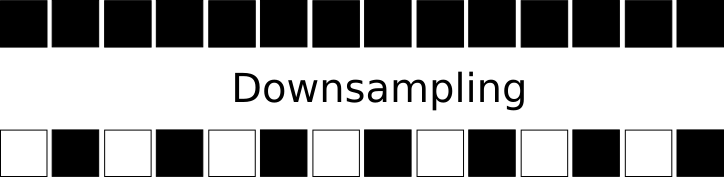
\includegraphics[width=0.7\linewidth]{images/downsampling}
				\label{fig:downsampling}
				\\Fonte: Elaborado pelo autor, 2021.
			\end{figure}
			
		\subsection{Caracterização dos processos de produção da voz humana}
			\par A fala possui três grandes áreas de estudo: A fisiológica, também conhecida como fonética articulatória, a acústica, referida como fonética acústica, e ainda, a perceptual, que cuida da percepção  da  fala \cite{kremer2014eficiencia}. Neste trabalho, o foco será apenas na questão acústica, pois não serão analisados aspectos da fisiologia relacionada à voz, mas sim os sinais sonoros propriamente ditos.
			
			\subsubsection{Sinais vozeados \textit{versus} não-vozeados}

			\par Quando da análise dos sinais de voz, consideram-se as partes vozeadas e não-vozeadas. Aquelas são produzidas com a ajuda da vibração quase periódica das pregas vocais, enquanto estas praticamente não contam com participação regrada da referida estrutura.
			
			\subsubsection{Frequência fundamental da voz}
				\par Também conhecida como $F_0$, é o componente periódico resultante da vibração das pregas vocais. Em termos de percepção, se pode interpretar $F_0$ como o tom da voz, isto é, a frequência de \textit{pitch} \cite{kremer2014eficiencia}. Vozes agudas tem uma frequência de \textit{pitch} alto, enquanto vozes mais graves tem baixa. A alteração da frequência (jitter) e/ou intensidade (shimmer) do \textit{pitch} durante a fala é definida como entonação,  porém, também pode indicar algum distúrbio ou doença relacionada ao trato vocal \cite{WERTZNER2005}.
				
				\par A frequência fundamental da voz é o número de vezes na qual uma forma de onda característica, que reflete a excitação pulmonar moldada pelas pregas vocais, se repete por unidade de tempo. Sendo assim, as medidas de $F_0$ geralmente são apresentadas em Hz \cite{freitas2013avaliaccao}.
			
				\par A medição de $F_0$ está sujeita a contaminações surgidas das variações naturais de \textit{pitch} típicas da voz humana \cite{freitas2013avaliaccao}. A importância de se medir $F_0$ corretamente vem do fato de que, além de carregar boa parte da informação da fala, ela é a base para construção das outras frequências que compõe os sinais de voz, que são múltiplas de $F_0$.
				
				\subsubsection{Formantes}
					\par O sinal de excitação que atravessa as pregas vocais é rico em harmônicas, isto é, frequências múltiplas da fundamental. Tais harmônicas podem ser atenuadas ou amplificadas, em função da estrutura dos tratos vocal e nasal de cada locutor. Particularmente, o primeiro formante ($F_1$), relaciona-se à  amplificação  sonora  na  cavidade  oral  posterior  e  à  posição  da  língua  no  plano  vertical;  o segundo  formante  ($F_2$)  à  cavidade  oral  anterior  e  à  posição  da  língua  no  plano  horizontal; o terceiro  formante  ($F_3$)  relaciona-se  às  cavidades  à  frente  e  atrás  do  ápice  da  língua e, finalmente,  o  quarto formante  ($F_4$) relaciona-se  ao  formato  da  laringe  e  da  faringe  na  mesma  altura  \cite{valencca2014analise}. Formantes caracterizam fortemente os locutores, pois cada indivíduo possui um formato de trato vocal e nasal. Assim, tais frequências, que podem ser capturadas com ferramentas diversas, a exemplo da Transformada \textit{Wavelet}, são de suma importância na área de verificação de locutores.

\subsection{Distâncias Euclidiana e Manhattan}
    \par Por definição, as distâncias Euclidiana ($D_E$) e Manhattan ($D_M$) entre dois vetores $x[\cdot]$ e $y[\cdot]$ de tamanho $M$ são dadas, respectivamente, por:
    \begin{equation}
     D_E = \sqrt{\sum\limits_{i=0}^{M-1}(x_i - y_i)^2}
    \end{equation}
	e
    \begin{equation}
        D_M = \sqrt{\sum\limits_{i=0}^{M-1}|x_i - y_i|}   
        \qquad. 
    \end{equation}

\subsection{Escalas e energias dos sinais}
	\par A energia de um sinal digital $s[\cdot]$ com $M$ amostras é definida como
	\begin{equation}
	E = \sum\limits_{i=0}^{M-1}(s_i)^2 \qquad.   
	\end{equation}
	$E$ pode ainda sofrer normalizações e ter a sua mensuração restrita a uma parte específica do sinal sob análise. Possibilidades para tais restrições podem, por exemplo, envolver a escala BARK \cite{doi:10.1121-1.1908630} e MEL \cite{beranek1949acoustic} que serão utilizadas neste trabalho.
	\subsubsection{A escala BARK}
		\par BARK foi definida tendo em mente vários tipos de sinais acústicos. Essa escala corresponde ao conjunto de 25 bandas críticas da audição humana. Suas frequências-base de audiometria são, em Hz: \textbf{20, 100, 200, 300, 400, 510, 630, 770, 920, 1080, 1270, 1480, 1720, 2000, 2320, 2700, 3150, 3700, 4400, 5300, 6400, 7700, 9500, 12000, 15500}. Nessa escala,os sinais digitais no domínio temporal atravessam filtros passa-faixas \cite{bosi2002introduction} para os quais o início e o final da banda de passagem correspondem à frequências-base consecutivas resultando em um vetor de características com 24 coeficientes e, em seguida, as energias dos sinais filtrados são utilizadas como características descritivas de propriedades do sinal sob análise, como mostrado na Figura \ref{fig:barkfeaturevect}.
		\begin{figure}[h]
			\centering
			\caption{Cálculo de vetores de características com BARK}
			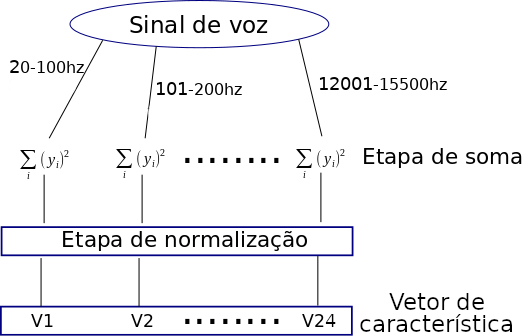
\includegraphics[width=0.6\linewidth]{images/barkFeatureVect}
			\label{fig:barkfeaturevect}
			\\Fonte: Elaborado pelo autor, 2021.
		\end{figure}
	\subsubsection{A escala MEL}
		\par Escala Mel, advinda do termo \textit{melody}, é uma adaptação da escala Bark para sinais de voz. Dentre as várias implementações de bandas críticas a escolhida foi a implementação que contém os valores em Hz: \textbf{20, 160, 394, 670, 1000, 1420, 1900, 2450, 3120, 4000, 5100, 6600, 9000, 14000}.
		\par A variante que será usada neste trabalho é conhecida como \textit{Mel-frequency cepstral coefficients}(MFCC) a qual inclui, além dos intervalos definidos, uma diminuição da correlação entre os componentes gerados via aplicação da Transformada Discreta Cosseno (DCT) \cite{salomon2007data} ou da Análise de Componentes Principais (PCA) \cite{jolliffe2006principal} seguida de duas derivações no vetor de características resultando em um total de 11 coeficientes. Nesse trabalho foi escolhida a DCT, no entanto, PCA poderia também ser escolhida sem prejuízos, o uso de uma ou outra depende da preferência do autor.
		\par Novamente, desconsiderando qualquer etapa intermediária que possa ser adicionada, as energias calculadas nos intervalos definidos na escala MEL podem, por si mesmas, constituir um vetor de características, como mostrado na Figura \ref{fig:barkfeaturevect}.
		\begin{figure}[h]
			\centering
			\caption{Cálculo de vetores de características com MEL}
			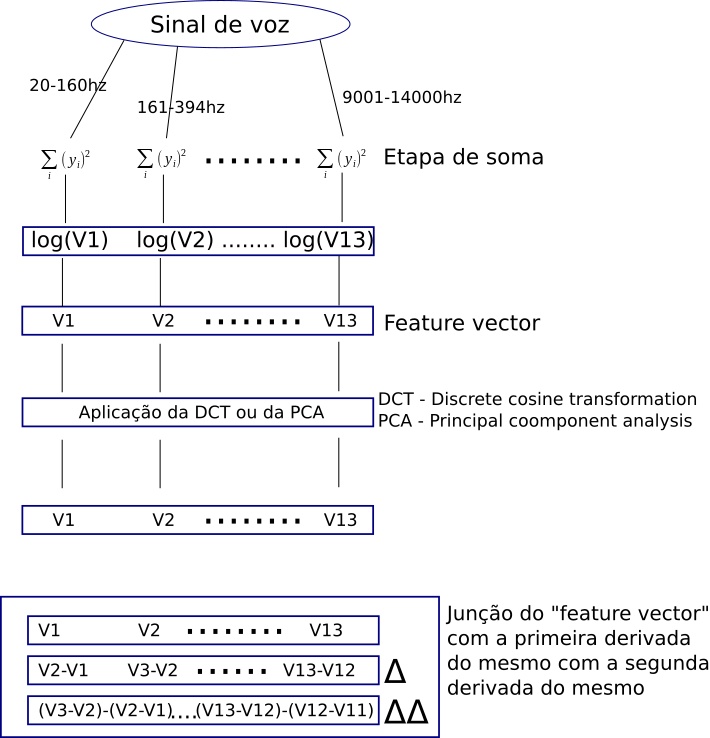
\includegraphics[width=0.8\linewidth]{images/melFeatureVect}
			\label{fig:melfeaturevect}
			\\Fonte: Elaborado pelo autor, 2021.
		\end{figure}
	
		\subsection{Filtros digitais \textit{wavelet}}
			\par Filtros digitais \textit{wavelet} têm sido utilizados com sucesso para suprir as deficiências de janelamento de sinal apresentadas pelas Transformadas de Fourier e de Fourier de Tempo Reduzido. \textit{Wavelets} contam com variadas funções-filtro e têm tamanho de janela variável, o que permite uma análise multirresolução \cite{Rod5254905}. Particularmente, as \textit{wavelets} proporcionam a análise do sinal de forma detalhada tanto no espectro de baixa frequência quanto no de alta contando com diferentes funções-base não periódicas diferentemente da tradicional transformada de Fourrier que utilizam somente as bases periódicas senoidal e cossenoidal.
			
			\par É importante observar que, quando se trata de Transformadas \textit{Wavelet}, seis elementos estão presentes: dois filtros de análise, dois filtros de síntese e as funções ortogonais \textit{scaling} e \textit{wavelet}. No tocante a sua aplicação, só a transformada direta, e não a inversa, será usada na construção dos vetores de características. Portanto, os filtros de síntese, a função \textit{scaling} e a função \textit{wavelet} não serão elementos abordados aqui: eles somente interessariam caso houvesse a necessidade da transformada inversa.

			\par No contexto dos filtros digitais baseados em \textit{wavelets}, o tamanho da janela recebe o nome de \textbf{suporte}. Janelas definem o tamanho do filtro que será aplicado ao sinal. Quando esse é pequeno (limitado), se diz que a janela tem \textbf{um suporte compacto} \cite{robi2003}.
		
			\par Se diz que uma \textit{wavelet} tem boa \textbf{resposta em frequência} quando, na aplicação da mesma para filtragem, não são causadas muitas pertubações indesejadas ao sinal, no domínio da frequência. Os filtros \textit{wavelet} de Daubechies \cite{daubechies1992ten} se destacam nesse quesito por serem \textit{maximamente planos} (\textit{maximally-flat}) \cite{butterworth1930} \cite{bianchi2007electronic} nos platôs de resposta em frequência como indicado na Figura \ref{fig:daubechies} ao contrário do que ocorre na Figura \ref{fig:nomaximallyflat}.

			\begin{figure}[h]
				\centering
				\caption{Platôs maximamente planos em um filtro digital: característica da família de Daubechies}
				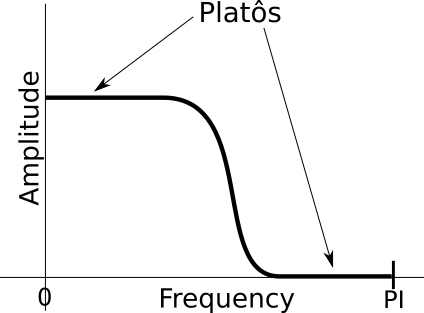
\includegraphics[width=0.3\linewidth]{images/daubechies}
				\label{fig:daubechies}
				\\Fonte: Elaborado pelo autor, 2021.
			\end{figure}

			\begin{figure}[h]
				\centering
				\caption{Platôs não maximamente planos de um filtro digital: características de outros filtros \textit{wavelet}, distintos da família de Daubechies}
				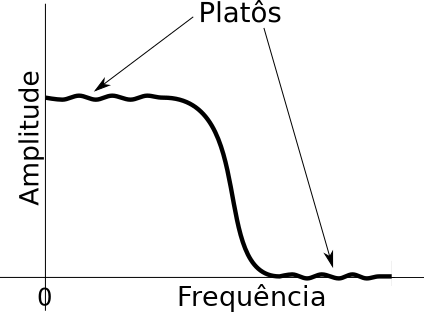
\includegraphics[width=0.3\linewidth]{images/noMaximallyFlat}
				\label{fig:nomaximallyflat}
				\\Fonte: Elaborado pelo autor, 2021.
			\end{figure}
		
			\par Além da resposta em frequência, na aplicação de um filtro digital \textit{wavelet} também é possível considerar a \textbf{resposta em fase}, que constitui um atraso ou adiantamento do sinal filtrado em relação ao sinal original, ambos no domínio temporal. Esse deslocamento pode ser \textbf{linear}, \textbf{quase linear} ou \textbf{não linear}: 
			
			\begin{itemize}
				\item na resposta em fase \textbf{linear}, há o mesmo deslocamento de fase para todos os componentes do sinal;
				\item quando a resposta em fase é \textbf{quase linear} existe uma pequena diferença no deslocamento dos diferentes componentes do sinal;
				\item finalmente, quando a resposta é \textbf{não linear}, acontece um deslocamento significativamente heterogêneo para as diferentes frequências que compõe o sinal.
				\end{itemize}
			
			\par Idealmente, é desejável que todo filtro apresente boa resposta em frequência e em fase linear. Características de fase e frequência de algumas famílias de filtros \textit{wavelet} constam na Tabela \ref{tab:waveletsProperties}.
			
			\begin{table}[h]
	\centering
	\caption{Algumas das \textit{wavelets} mais usadas e suas propriedades}
	\begin{tabular}{|c|p{75mm}|c|}
			\hline 
			\textbf{Wavelet} & \textbf{Resposta em frequência} & \textbf{Resposta em fase} \\ 
			\hline 
			Haar & Pobre &  Linear \\ 
			\hline 
			Daubechies & mais próxima da ideal à medida que o \newline  suporte aumenta; \textit{maximally-flat}  &  Não linear \\ 
			\hline 
			Symmlets & mais próxima da ideal à medida que o \newline  suporte aumenta; não \textit{maximally-flat}  & Quase linear \\ 
			\hline 
			Coiflets & mais próxima da ideal à medida que o \newline  suporte aumenta; não \textit{maximally-flat}  & Quase linear \\ 
			\hline 
	\end{tabular} 
	\label{tab:waveletsProperties}
	\\Fonte: Elaborado pelo autor, 2021.
\end{table}


		\subsubsection{O algoritmo de Mallat para a Transformada \textit{Wavelet}}
			\par Baseando-se no artigo \citetext{7079589}, percebe-se que algoritmo de Mallat faz com que aplicação das \textit{wavelets} seja uma simples multiplicação de matrizes. O sinal que deve ser transformado se torna uma matriz linear vertical. Os filtros passa-baixa e passa-alta tornam-se, nessa ordem, linhas de uma matriz quadrada que será completada segundo regras que serão mostradas mais adiante. É importante que essa matriz quadrada tenha a mesma dimensão que o sinal a ser transformado.
		
			\par Interessantemente, para que seja possível a transformação \textit{wavelet}, basta ter disponível o vetor do filtro passa-baixas calculado a partir da \textit{mother wavelet}, que é a função geradora desse filtro, já que o passa-alta pode ser construído a partindo-se da ortogonalidade do primeiro.
			
			\par Determinar a ortogonal de um vetor significa construir um vetor, tal que, o produto escalar do vetor original com sua respectiva ortogonal seja nulo.
			
			\par Considerando $h[\cdot]$ como sendo o vetor do filtro passa-baixas e $g[\cdot]$ seu correspondente ortogonal, tem-se que $h[\cdot] \cdot g[\cdot] = 0 \qquad .$
			\par Portanto, se $h[\cdot]=[a, b, c, d]$ então seu ortogonal será $g[\cdot]=[d, -c, b, -a]$ pois:
			$$
				h[\cdot] \cdot g[\cdot]  =  [a, b, c, d] \cdot [d, -c, b, -a] = (a \cdot d) + (b \cdot (-c)) + (c \cdot b) + (d \cdot (-a)) = ad - ad + bc - bc = 0 \qquad.
			$$

			\par A título de exemplo, considera-se:
			\begin{itemize}
				\item o filtro passa baixa baseado na \textit{wavelet} Haar: $h[\cdot] = [\frac{1}{\sqrt{2}}, \frac{1}{\sqrt{2}}]$
				\item o seu respectivo vetor ortogonal: $g[\cdot] = [\frac{1}{\sqrt{2}}, \frac{-1}{\sqrt{2}}]$
				\item e também o seguinte sinal-exemplo de entrada: $s = \{1,2,3,4\}$
			\end{itemize}

			\par Se o tamanho do sinal a ser tratado é quatro e se pretende-se aplicar o filtro Haar, a seguinte matriz de coeficientes é construída:
			\begin{equation}
				\begin{pmatrix}
					\frac{1}{\sqrt{2}}, \frac{1}{\sqrt{2}}, 0, 0\\
					\frac{1}{\sqrt{2}}, \frac{-1}{\sqrt{2}}, 0, 0\\
					0, 0, \frac{1}{\sqrt{2}}, \frac{1}{\sqrt{2}}\\
					0, 0, \frac{1}{\sqrt{2}}, \frac{1}{\sqrt{2}}
					\label{eq:haarFilters}
				\end{pmatrix} 
			\end{equation}
			\par Tendo em vista que a dimensão do sinal sob análise é diferente da dimensão do filtro, basta completar cada uma das linhas da matriz de coeficientes com zeros. A matriz é montada de forma que ela seja ortogonal.

			\par Montada a matriz de filtros, segue-se com os cálculos da transformada:
			\begin{equation}
				\begin{pmatrix}
					\frac{1}{\sqrt{2}}, \frac{1}{\sqrt{2}}, 0, 0\\
					\frac{1}{\sqrt{2}}, \frac{-1}{\sqrt{2}}, 0, 0\\
					0, 0, \frac{1}{\sqrt{2}}, \frac{1}{\sqrt{2}}\\
					0, 0, \frac{1}{\sqrt{2}}, \frac{1}{\sqrt{2}}\\
				\end{pmatrix} 
				\cdot
				\begin{pmatrix}
					1\\
					2\\
					3\\
					4\\
				\end{pmatrix} 
				=
				\begin{pmatrix}
					\frac{3}{\sqrt{2}}\\
					\frac{-1}{\sqrt{2}}\\
					\frac{7}{\sqrt{2}}\\
					\frac{-1}{\sqrt{2}}
				\end{pmatrix}
				\label{eq:haarMultiplic}
			\end{equation}
			
			\par Realizada a multiplicação, é necessário montar o sinal filtrado. Isso é feito escolhendo, dentro do resultado, valores alternadamente de forma que o vetor resultante seja:

			\begin{equation}
				resultado = \Big[
				\frac{3}{\sqrt{2}},
				\frac{7}{\sqrt{2}},
				\frac{-1}{\sqrt{2}},
				\frac{-1}{\sqrt{2}}
				\Big]\qquad.
				\label{eq:haarResult}
			\end{equation}
			
			\par Percebe-se que, na transformação descrita nas Equações \ref{eq:haarFilters}, \ref{eq:haarMultiplic} e \ref{eq:haarResult}, a \textbf{aplicação dos filtros sobre o vetor de entrada ocorreu apenas uma vez}. Sendo assim, se diz que o sinal recebeu uma \textbf{transformação de nível 1}. A cada transformação, há uma separação do sinal em dois componentes: o de baixa e o de alta frequência.
			
			\par Embora haja um limite, que será mencionado adiante, é possível aplicar mais de um nível de decomposição ao sinal. Para que se possa fazer isso, a Transformada \textit{Wavelet} nível 2 deve considerar apenas a parte de baixas frequências da primeira transformada; a transformada de nível 3 deve considerar apenas a parte de baixas frequências da transformada nível 2, e assim consecutivamente.
			
			\par Nos exemplos numéricos mostrados nas Tabelas \ref{tab:regularWaveletExample}, \ref{tab:packetWaveletExampleLF} e \ref{tab:packetWaveletExampleHF}, usou-se um filtro normalizado cujos coeficientes são $\{\dfrac{1}{2},-\dfrac{1}{2}\}$. Os dados destacados em \textbf{verde} correspondem ao \textbf{vetor original} que será tratado. Cada uma das linhas são os resultados das transformações nos níveis 1, 2, 3 e 4, respectivamente. As partes em \textbf{azul} correspondem à porção de \textbf{baixas frequências}, enquanto que as partes em \textbf{amarelo} correspondem às porções de \textbf{altas frequências}.
			
			\par Percebe-se que na Tabela \ref{tab:regularWaveletExample}, a partir da transformação nível 2, apenas as partes de baixa frequência são modificadas. Isso implica que, no momento da implementação do algoritmo de Mallat \textbf{para níveis maiores que 1}, a abordagem será \textbf{recursiva}. Em outras palavras, a partir do nível 1 se deve aplicar Mallat apenas às porções de baixas-frequências geradas pela transformação anterior.
			
			\begin{table}[h]
	\fontsize{9}{\baselineskip} \selectfont
	\newcommand{\mc}[3]{\multicolumn{#1}{#2}{#3}}
	\definecolor{tcA}{rgb}{0.65098,0.65098,0.65098}
	\definecolor{tcD}{rgb}{1,0.94902,0}
	\definecolor{tcC}{rgb}{0,0.5,1}
	\definecolor{tcB}{rgb}{0.447059,0.74902,0.266667}
	\begin{center}
		\caption{Exemplo numérico da transformação \textit{wavelet} aplicada a um vetor}
		\begin{tabular}{c|ccccccccccccccc|c}
			% use packages: color,colortbl
			\mc{1}{>{\columncolor{tcA}}c|}{\textbf{Sinal}} & \mc{1}{>{\columncolor{tcB}}c}{\textbf{32}} & \mc{1}{>{\columncolor{tcB}}c}{\textbf{10}} & \mc{1}{>{\columncolor{tcB}}c}{\textbf{20}} & \mc{1}{>{\columncolor{tcB}}c}{\textbf{38}} & \mc{1}{>{\columncolor{tcB}}c}{\textbf{37}} & \mc{1}{>{\columncolor{tcB}}c}{\textbf{28}} & \mc{1}{>{\columncolor{tcB}}c}{\textbf{38}} & \mc{1}{>{\columncolor{tcB}}c}{\textbf{34}} & \mc{1}{>{\columncolor{tcB}}c}{\textbf{18}} & \mc{1}{>{\columncolor{tcB}}c}{\textbf{24}} & \mc{1}{>{\columncolor{tcB}}c}{\textbf{24}} & \mc{1}{>{\columncolor{tcB}}c}{\textbf{9}} & \mc{1}{>{\columncolor{tcB}}c}{\textbf{23}} & \mc{1}{>{\columncolor{tcB}}c}{\textbf{24}} & \mc{1}{>{\columncolor{tcB}}c}{\textbf{28}} & \mc{1}{>{\columncolor{tcB}}c}{\textbf{34}}\\
			\hline
			
			\mc{1}{>{\columncolor{tcA}}c|}{Nível 01} & \mc{1}{>{\columncolor{tcC}}c}{21} & \mc{1}{>{\columncolor{tcC}}c}{29} & \mc{1}{>{\columncolor{tcC}}c}{32,5} & \mc{1}{>{\columncolor{tcC}}c}{36} & \mc{1}{>{\columncolor{tcC}}c}{21} & \mc{1}{>{\columncolor{tcC}}c}{16,5} & \mc{1}{>{\columncolor{tcC}}c}{23,5} & \mc{1}{>{\columncolor{tcC}}c}{31} & \mc{1}{>{\columncolor{tcD}}c}{11} & \mc{1}{>{\columncolor{tcD}}c}{-9} & \mc{1}{>{\columncolor{tcD}}c}{4,5} & \mc{1}{>{\columncolor{tcD}}c}{2} & \mc{1}{>{\columncolor{tcD}}c}{-3} & \mc{1}{>{\columncolor{tcD}}c}{7,5} & \mc{1}{>{\columncolor{tcD}}c}{-0,5} & \mc{1}{>{\columncolor{tcD}}c}{-3}\\
			\hline
			
			\mc{1}{>{\columncolor{tcA}}c|}{Nível 02} & \mc{1}{>{\columncolor{tcC}}c}{25} & \mc{1}{>{\columncolor{tcC}}c}{34,25} & \mc{1}{>{\columncolor{tcC}}c}{18,75} & \mc{1}{>{\columncolor{tcC}}c}{27,25} & \mc{1}{>{\columncolor{tcD}}c}{-4} & \mc{1}{>{\columncolor{tcD}}c}{-1,75} & \mc{1}{>{\columncolor{tcD}}c}{2,25} & \mc{1}{>{\columncolor{tcD}}c}{-3,75} & \mc{1}{>{\columncolor{tcD}}c}{11} & \mc{1}{>{\columncolor{tcD}}c}{-9} & \mc{1}{>{\columncolor{tcD}}c}{4,5} & \mc{1}{>{\columncolor{tcD}}c}{2} & \mc{1}{>{\columncolor{tcD}}c}{-3} & \mc{1}{>{\columncolor{tcD}}c}{7,5} & \mc{1}{>{\columncolor{tcD}}c}{-0,5} & \mc{1}{>{\columncolor{tcD}}c}{-3}\\
			\hline
			
			\mc{1}{>{\columncolor{tcA}}c|}{Nível 03} & \mc{1}{>{\columncolor{tcC}}c}{29,62} & \mc{1}{>{\columncolor{tcC}}c}{23} & \mc{1}{>{\columncolor{tcD}}c}{-4,625} & \mc{1}{>{\columncolor{tcD}}c}{-4,25} & \mc{1}{>{\columncolor{tcD}}c}{-4} & \mc{1}{>{\columncolor{tcD}}c}{-1,75} & \mc{1}{>{\columncolor{tcD}}c}{2,25} & \mc{1}{>{\columncolor{tcD}}c}{-3,75} & \mc{1}{>{\columncolor{tcD}}c}{11} & \mc{1}{>{\columncolor{tcD}}c}{-9} & \mc{1}{>{\columncolor{tcD}}c}{4,5} & \mc{1}{>{\columncolor{tcD}}c}{2} & \mc{1}{>{\columncolor{tcD}}c}{-3} & \mc{1}{>{\columncolor{tcD}}c}{7,5} & \mc{1}{>{\columncolor{tcD}}c}{-0,5} & \mc{1}{>{\columncolor{tcD}}c}{-3}\\
			\hline
			
			\mc{1}{>{\columncolor{tcA}}c|}{Nível 04} & \mc{1}{>{\columncolor{tcC}}c}{26,3125} & \mc{1}{>{\columncolor{tcD}}c}{3,3125} & \mc{1}{>{\columncolor{tcD}}c}{-4,625} & \mc{1}{>{\columncolor{tcD}}c}{-4,25} & \mc{1}{>{\columncolor{tcD}}c}{-4} & \mc{1}{>{\columncolor{tcD}}c}{-1,75} & \mc{1}{>{\columncolor{tcD}}c}{2,25} & \mc{1}{>{\columncolor{tcD}}c}{-3,75} & \mc{1}{>{\columncolor{tcD}}c}{11} & \mc{1}{>{\columncolor{tcD}}c}{-9} & \mc{1}{>{\columncolor{tcD}}c}{4,5} & \mc{1}{>{\columncolor{tcD}}c}{2} & \mc{1}{>{\columncolor{tcD}}c}{-3} & \mc{1}{>{\columncolor{tcD}}c}{7,5} & \mc{1}{>{\columncolor{tcD}}c}{-0,5} & \mc{1}{>{\columncolor{tcD}}c}{-3}
		\end{tabular}
		\label{tab:regularWaveletExample}
		\fontsize{12}{\baselineskip} \selectfont
		\\Fonte: Elaborado pelo autor, 2021.
	\end{center}
\end{table}

		\subsubsection{O algoritmo de Mallat e a Transformada \textit{Wavelet-Packet}}
			\par Na Transformada \textit{Wavelet-Packet}, os filtros aplicados são os mesmos da Transformada \textit{Wavelet} e o procedimento recursivo de cálculo também é o mesmo, no entanto, realizada a transformação de nível 1, a transformada de nível 2 deve ser aplicada aos componentes de baixa e de alta frequência. Sendo assim a Transformada \textit{Wavelet-Packet} obtém um nível de detalhes em todo o espectro de frequência, maior do que uma transformação regular. 
			
			\par Os exemplos mostrados nas Tabelas \ref{tab:packetWaveletExampleLF} e \ref{tab:packetWaveletExampleHF} permitem perceber como se dão as transformações na porção de \textbf{baixa} e de \textbf{alta} frequências, respectivamente, após a transformação \textit{wavelet-packet} de nível 1, 2, 3 e 4.

			\par Devido ao \textit{downsampling} aplicado às porções de alta frequência, essas partes acabam por ficar ``espelhadas'' no espectro \cite{Jensen_2001}, ou seja, suas sequências ficam invertidas. Para resolver esse problema e preservar a ordem das sub-bandas no sinal transformado, os filtros são aplicados em ordem inversa nas porções de alta frequência. Isso altera como o algoritmo de Mallat deve ser implementado para a Transformada \textit{Wavelet-Packet}, já que dessa vez é preciso se atentar a ordem da aplicação dos filtros passa-alta e passa-baixa.

			\begin{table}[h]
	\newcommand{\mc}[3]{\multicolumn{#1}{#2}{#3}}
	\definecolor{tcA}{rgb}{0.65098,0.65098,0.65098}
	\definecolor{tcD}{rgb}{1,0.94902,0}
	\definecolor{tcC}{rgb}{0,0.4,0.701961}
	\definecolor{tcB}{rgb}{0.447059,0.74902,0.266667}
	\begin{center}
		\begin{tabular}{l|llllllll|}
			% use packages: color,colortbl
			\mc{1}{>{\columncolor{tcA}}l|}{\textbf{Sinal}} & \mc{1}{>{\columncolor{tcB}}l}{\textbf{32}} & \mc{1}{>{\columncolor{tcB}}l}{\textbf{10}} & \mc{1}{>{\columncolor{tcB}}l}{\textbf{20}} & \mc{1}{>{\columncolor{tcB}}l}{\textbf{38}} & \mc{1}{>{\columncolor{tcB}}l}{\textbf{37}} & \mc{1}{>{\columncolor{tcB}}l}{\textbf{28}} & \mc{1}{>{\columncolor{tcB}}l}{\textbf{38}} & \mc{1}{>{\columncolor{tcB}}l|}{\textbf{34}}\\
			\hline
			
			\mc{1}{>{\columncolor{tcA}}l|}{Nivel 01} & \mc{1}{>{\columncolor{tcC}}l}{21} & \mc{1}{>{\columncolor{tcC}}l}{29} & \mc{1}{>{\columncolor{tcC}}l}{32,5} & \mc{1}{>{\columncolor{tcC}}l}{36} & \mc{1}{>{\columncolor{tcC}}l}{21} & \mc{1}{>{\columncolor{tcC}}l}{16,5} & \mc{1}{>{\columncolor{tcC}}l}{23,5} & \mc{1}{>{\columncolor{tcC}}l|}{31}\\
			\hline
			
			\mc{1}{>{\columncolor{tcA}}l|}{Nivel 02} & \mc{1}{>{\columncolor{tcC}}l}{25} & \mc{1}{>{\columncolor{tcC}}l}{34,25} & \mc{1}{>{\columncolor{tcC}}l}{18,75} & \mc{1}{>{\columncolor{tcC}}l|}{27,25} & \mc{1}{>{\columncolor{tcD}}l}{-4} & \mc{1}{>{\columncolor{tcD}}l}{-1,75} & \mc{1}{>{\columncolor{tcD}}l}{2,25} & \mc{1}{>{\columncolor{tcD}}l|}{-3,75}\\
			\hline
			
			\mc{1}{>{\columncolor{tcA}}l|}{Nivel 03} & \mc{1}{>{\columncolor{tcC}}l}{29,62} & \mc{1}{>{\columncolor{tcC}}l|}{23} & \mc{1}{>{\columncolor{tcD}}l}{-4,625} & \mc{1}{>{\columncolor{tcD}}l|}{-4,25} & \mc{1}{>{\columncolor{tcD}}l}{-1,125} & \mc{1}{>{\columncolor{tcD}}l|}{3} & \mc{1}{>{\columncolor{tcC}}l}{-2,875} & \mc{1}{>{\columncolor{tcC}}l|}{-0,75}\\
			\hline
			
			\mc{1}{>{\columncolor{tcA}}l|}{Nivel 04} & \mc{1}{>{\columncolor{tcC}}l|}{26,3125} & \mc{1}{>{\columncolor{tcD}}l|}{3,3125} & \mc{1}{>{\columncolor{tcD}}l|}{-0,1875} & \mc{1}{>{\columncolor{tcC}}l|}{-4,4375} & \mc{1}{>{\columncolor{tcC}}l|}{0,9375} & \mc{1}{>{\columncolor{tcD}}l|}{-2,0625} & \mc{1}{>{\columncolor{tcD}}l|}{-1,0625} & \mc{1}{>{\columncolor{tcC}}l|}{-1,8125}\\
		\end{tabular}
		\caption{Exemplo numérico de \textit{wavelet-packet} Haar aplicada a um vetor (porção da baixas frequências)}
		\label{tab:packetWaveletExampleLF}
	\end{center}
\end{table}

\begin{table}[h]
	\newcommand{\mc}[3]{\multicolumn{#1}{#2}{#3}}
	\definecolor{tcA}{rgb}{0.65098,0.65098,0.65098}
	\definecolor{tcC}{rgb}{1,0.94902,0}
	\definecolor{tcD}{rgb}{0,0.4,0.701961}
	\definecolor{tcB}{rgb}{0.447059,0.74902,0.266667}
	\begin{center}
		\begin{tabular}{c|cccccccc}
			% use packages: color,colortbl
			\mc{1}{>{\columncolor{tcA}}c|}{\textbf{Sinal}} & \mc{1}{>{\columncolor{tcB}}c}{\textbf{18}} & \mc{1}{>{\columncolor{tcB}}c}{\textbf{24}} & \mc{1}{>{\columncolor{tcB}}c}{\textbf{24}} & \mc{1}{>{\columncolor{tcB}}c}{\textbf{9}} & \mc{1}{>{\columncolor{tcB}}c}{\textbf{23}} & \mc{1}{>{\columncolor{tcB}}c}{\textbf{24}} & \mc{1}{>{\columncolor{tcB}}c}{\textbf{28}} & \mc{1}{>{\columncolor{tcB}}c|}{\textbf{34}}\\\hline
			\mc{1}{>{\columncolor{tcA}}c|}{Nivel 01} & \mc{1}{>{\columncolor{tcC}}c}{11} & \mc{1}{>{\columncolor{tcC}}c}{-9} & \mc{1}{>{\columncolor{tcC}}c}{4,5} & \mc{1}{>{\columncolor{tcC}}c}{2} & \mc{1}{>{\columncolor{tcC}}c}{-3} & \mc{1}{>{\columncolor{tcC}}c}{7,5} & \mc{1}{>{\columncolor{tcC}}c}{-0,5} & \mc{1}{>{\columncolor{tcC}}c|}{-3}\\\hline
			\mc{1}{>{\columncolor{tcA}}c|}{Nivel 02} & \mc{1}{>{\columncolor{tcC}}c}{10} & \mc{1}{>{\columncolor{tcC}}c|}{1,25} & \mc{1}{>{\columncolor{tcC}}c}{-5,25} & \mc{1}{>{\columncolor{tcC}}c|}{1,25} & \mc{1}{>{\columncolor{tcD}}c}{1} & \mc{1}{>{\columncolor{tcD}}c|}{3,25} & \mc{1}{>{\columncolor{tcD}}c}{2,25} & \mc{1}{>{\columncolor{tcD}}c|}{-1,75}\\\hline
			\mc{1}{>{\columncolor{tcA}}c|}{Nivel 03} & \mc{1}{>{\columncolor{tcD}}c|}{5,625} & \mc{1}{>{\columncolor{tcD}}c|}{-2} & \mc{1}{>{\columncolor{tcC}}c|}{4,375} & \mc{1}{>{\columncolor{tcC}}c|}{-3,25} & \mc{1}{>{\columncolor{tcC}}c|}{-1,125} & \mc{1}{>{\columncolor{tcC}}c|}{2} & \mc{1}{>{\columncolor{tcD}}c|}{2,125} & \mc{1}{>{\columncolor{tcD}}c|}{0,25}\\\hline
			
			\mc{1}{>{\columncolor{tcA}}c|}{Nivel 04} & \mc{1}{>{\columncolor{tcD}}c|}{1,8125} & \mc{1}{>{\columncolor{tcC}}c|}{3,8125} & \mc{1}{>{\columncolor{tcC}}c|}{3,8125} & \mc{1}{>{\columncolor{tcD}}c|}{0,5625} & \mc{1}{>{\columncolor{tcD}}c|}{0,4375} & \mc{1}{>{\columncolor{tcC}}c|}{-1,5625} & \mc{1}{>{\columncolor{tcC}}c|}{0,9375} & \mc{1}{>{\columncolor{tcD}}c|}{1,1875}\\
		\end{tabular}
	\end{center}
	\caption{Exemplo numérico da transformação \textit{wavelet-packet} aplicada a um vetor}
	\label{tab:packetWaveletExampleHF}
\end{table}
			
			\par Para uma visualização mais completa, a Figura \ref{fig:haarWaveletExamples} pode ser consultada no apêndice deste documento.
			
			\subsection{Engenharia Paraconsistente de características}
				\par Nos processos de classificação, frequentemente surge a questão: ``Os vetores de características criados proporcionam uma boa separação de classes?''. A Engenharia Paraconsistente de Características, recém publicada \cite{8588433}, que usa a paraconsistência \cite{da1998elementos},  \cite{COSTA2000} é, em meio a outras técnicas, uma ferramenta que pode ser usada para responder essa questão.
				
				\par O processo inicia-se após a aquisição dos vetores de características para cada classe $C_n$. Se o número de classes presentes for, por exemplo, quatro então estas poderão ser representadas por $C_1, C_2, C_3, C_4$.
				\par Em seguida é necessário o cálculo de duas grandezas:
				
				\begin{itemize}
					\item a menor similaridade intraclasse, $\alpha$.
					\item a razão de sobreposição interclasse, $\beta$.
				\end{itemize}
			
				\par $\alpha$ indica o quanto de similaridade os dados têm entre si, dentro de uma mesma classe, enquanto $\beta$ é a razão de sobreposição entre diferentes classes. Idealmente, $\alpha$ deve ser maximizada e $\beta$ minimizada para que classificadores extremamente modestos apresentem uma acurácia interessante.
				
				\par Particularmente, para calcular $\alpha$ e $\beta$, é necessária a normalização dos vetores de características de forma que todos os seus componentes estejam no intervalo entre $0$ e $1$. Em seguida, a obtenção de $\alpha$ se dá selecionando-se os maiores e os menores valores de cada uma das posições de todos os vetores de características para cada classe, gerando assim um vetor para os valores maiores e outro para os menores.
				
				\par O \textbf{vetor de similaridade da classe}$(svC_n)$ é obtido fazendo-se a diferença item-a-item dos maiores em relação aos menores. Finalmente, e para cada classe, é obtida a média dos valores para cada vetor de similaridade, sendo que $\alpha$ é o menor valor dentre essas médias. A Figura \ref{fig:calculoalpha} contém uma ilustração do processo.
				
				\begin{figure}
					\centering
					\caption{Cálculo do coeficiente $\alpha$.}
			       	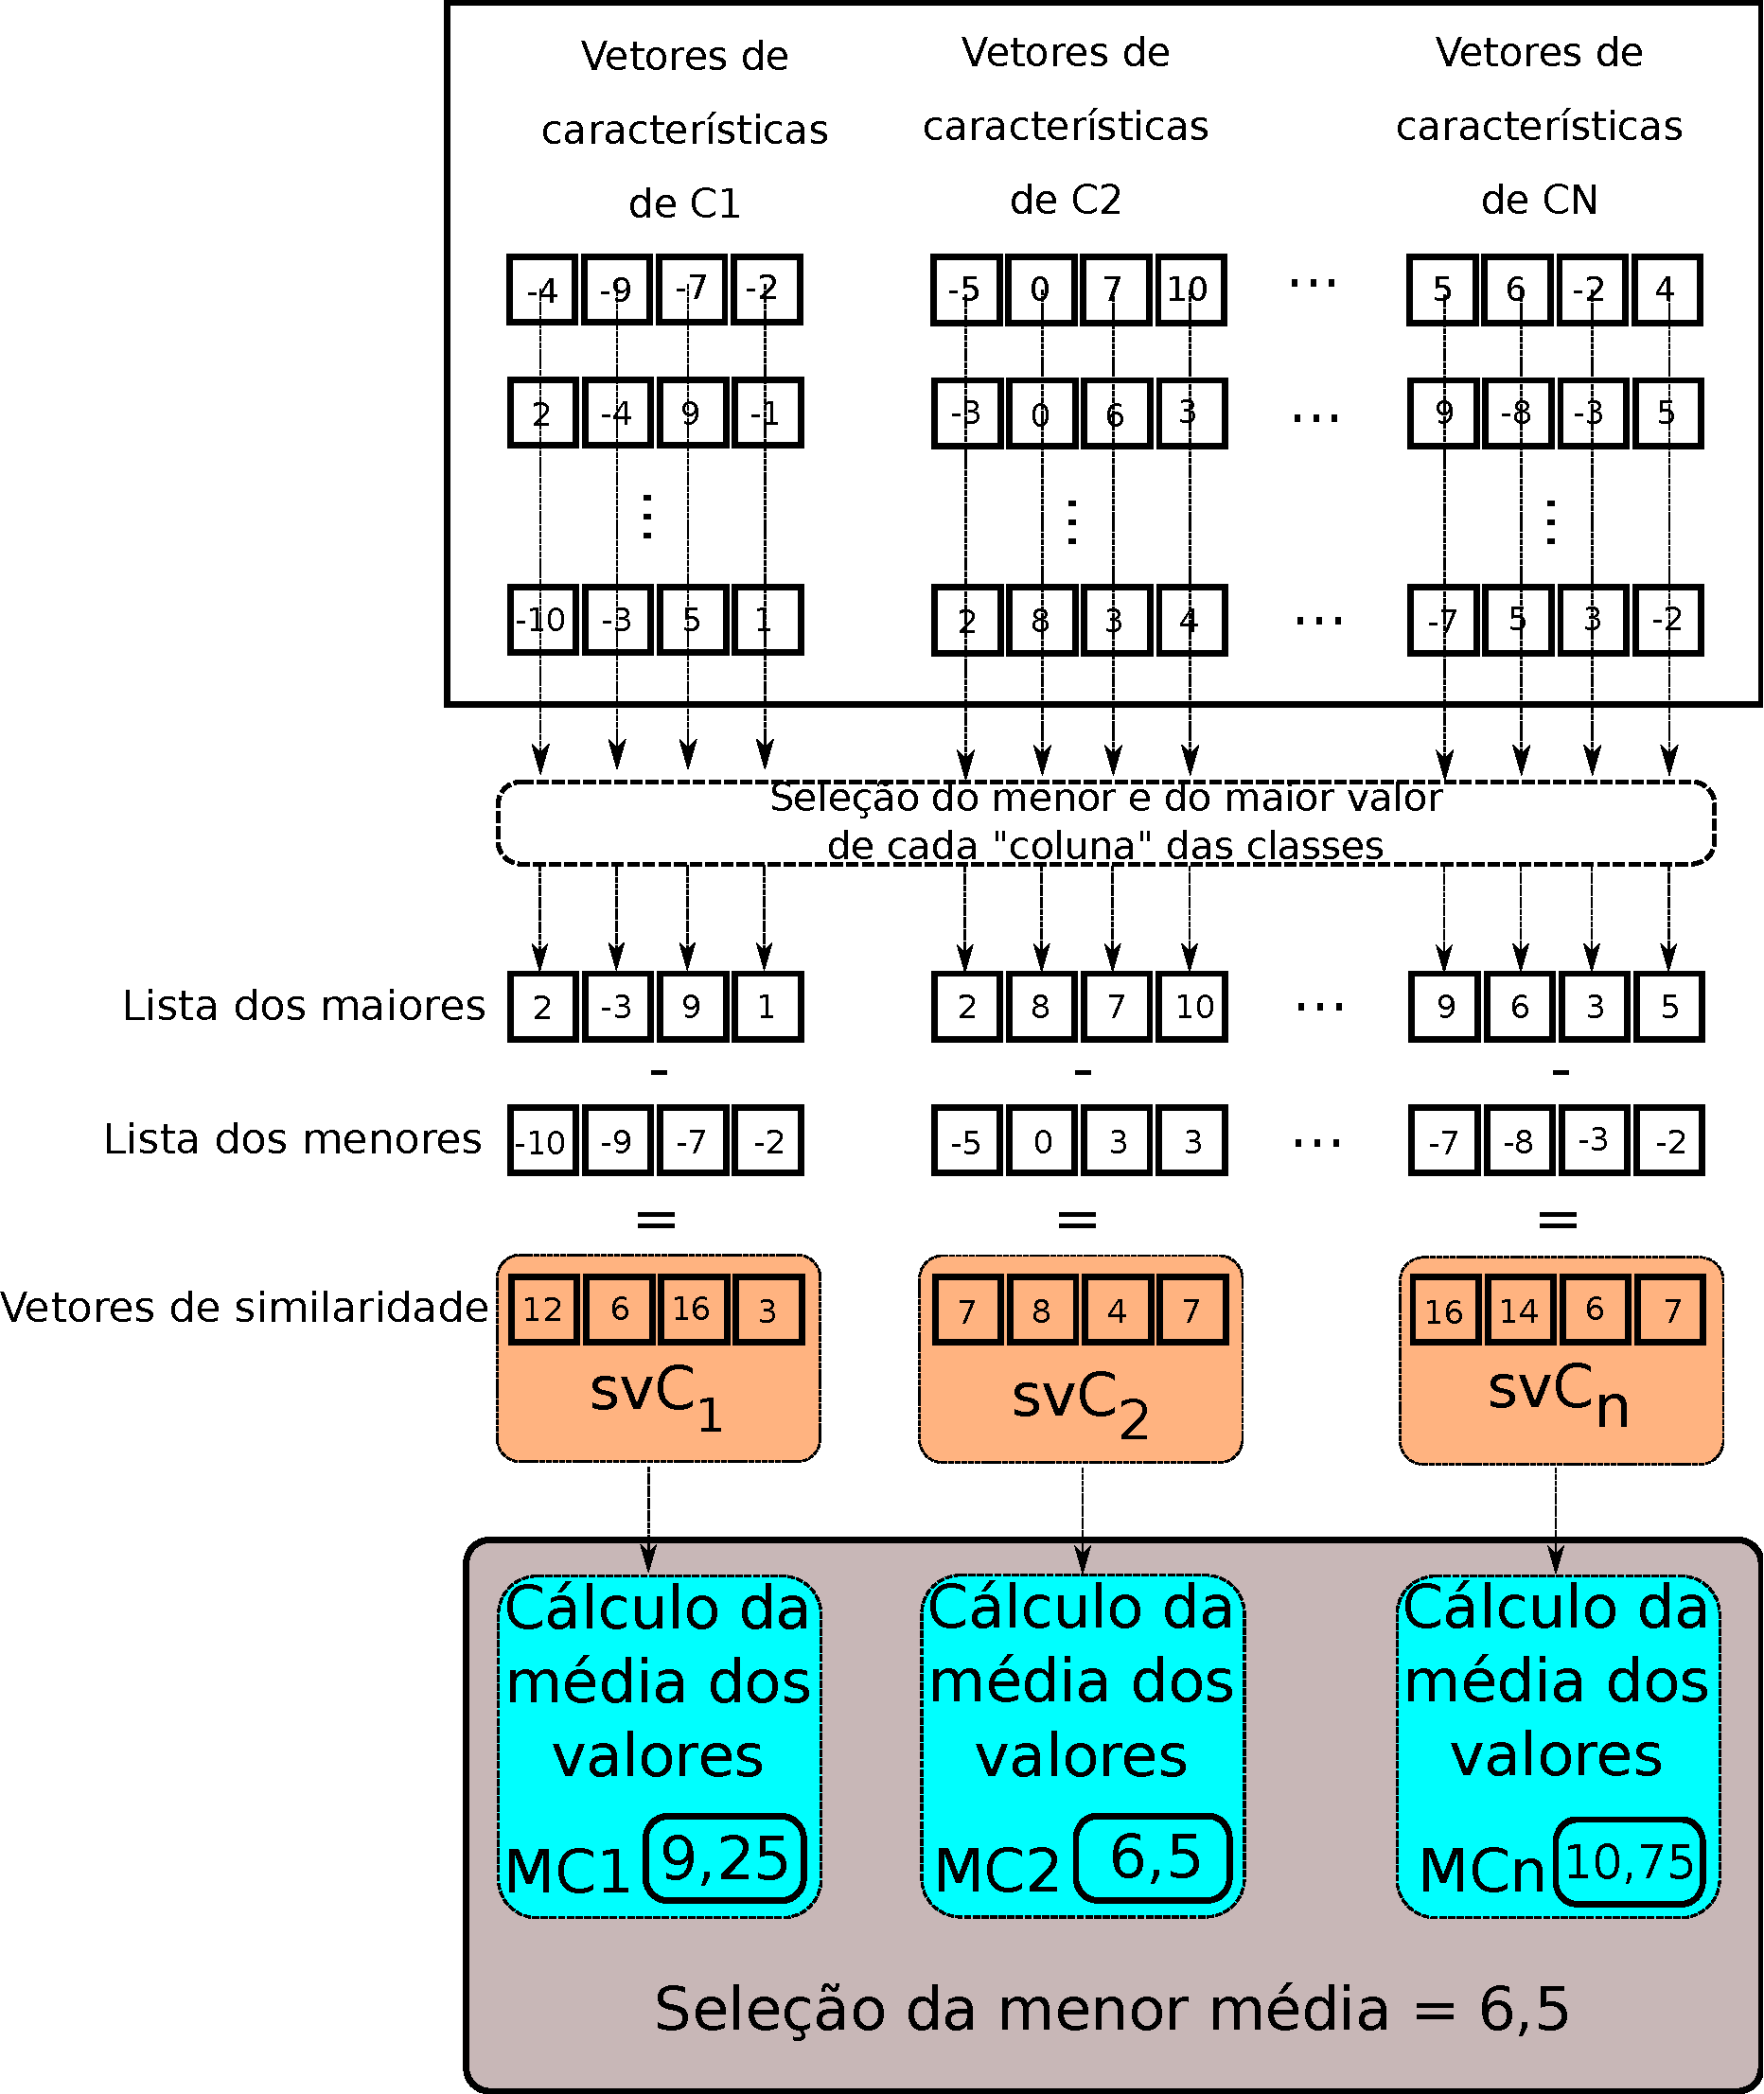
\includegraphics[width=0.77\linewidth]{images/calculoAlpha.pdf}
					\label{fig:calculoalpha}
					\\Fonte: Adaptado de \cite{8588433}.
				\end{figure}
				
				\par A obtenção de $\beta$, assim como ilustrado na Figura \ref{fig:betacalculation}, também se dá selecionando os maiores e os menores valores de cada uma das posições de todos os vetores de características de cada classe, gerando assim um vetor para os valores maiores e outro para os menores.
				
				\par Na sequência, realiza-se o cálculo de $R$ cujo valor é a quantidade de vezes que um valor do vetor de características de uma classe se encontra entre os valores maiores e menores de outra classe.
				
				\par Seja:
				\begin{itemize}
					\item N a quantidades de classes;
					\item X a quantidade de vetores de características por classe;
					\item T o tamanho do vetor de características.
				\end{itemize}
				
				\par Então, $F$, que é o número máximo de sobreposições possíveis entre classes, é dado por:
				\begin{equation}
						F=N.(N-1).X.T \qquad.
				\end{equation}
				\par Finalmente, $\beta$ é calculado da seguinte forma:
				\begin{equation}
					\beta=\dfrac{R}{F} \qquad.
				\end{equation}
			
				\par Neste ponto, é importante notar que $\alpha=1$ sugere fortemente que os vetores de características de cada classe são similares e representam suas respectivas classes precisamente. Complementarmente, $\beta=0$ sugere os vetores de características de classes diferentes não se sobrepõe \cite{8588433}.
				
				\begin{figure}[h]
					\centering
					\caption{Cálculo de $\beta$: Os itens destacados em azul e rosa são aqueles pertencentes a classe C1 e CN que se sobrepõe, em verde, a sobreposição é entre C1 e C2. Para cada sobreposição verificada soma-se 1 ao valor $R$. Essa comparação é feita para todos os vetores de características de cada uma das classes.}
		    		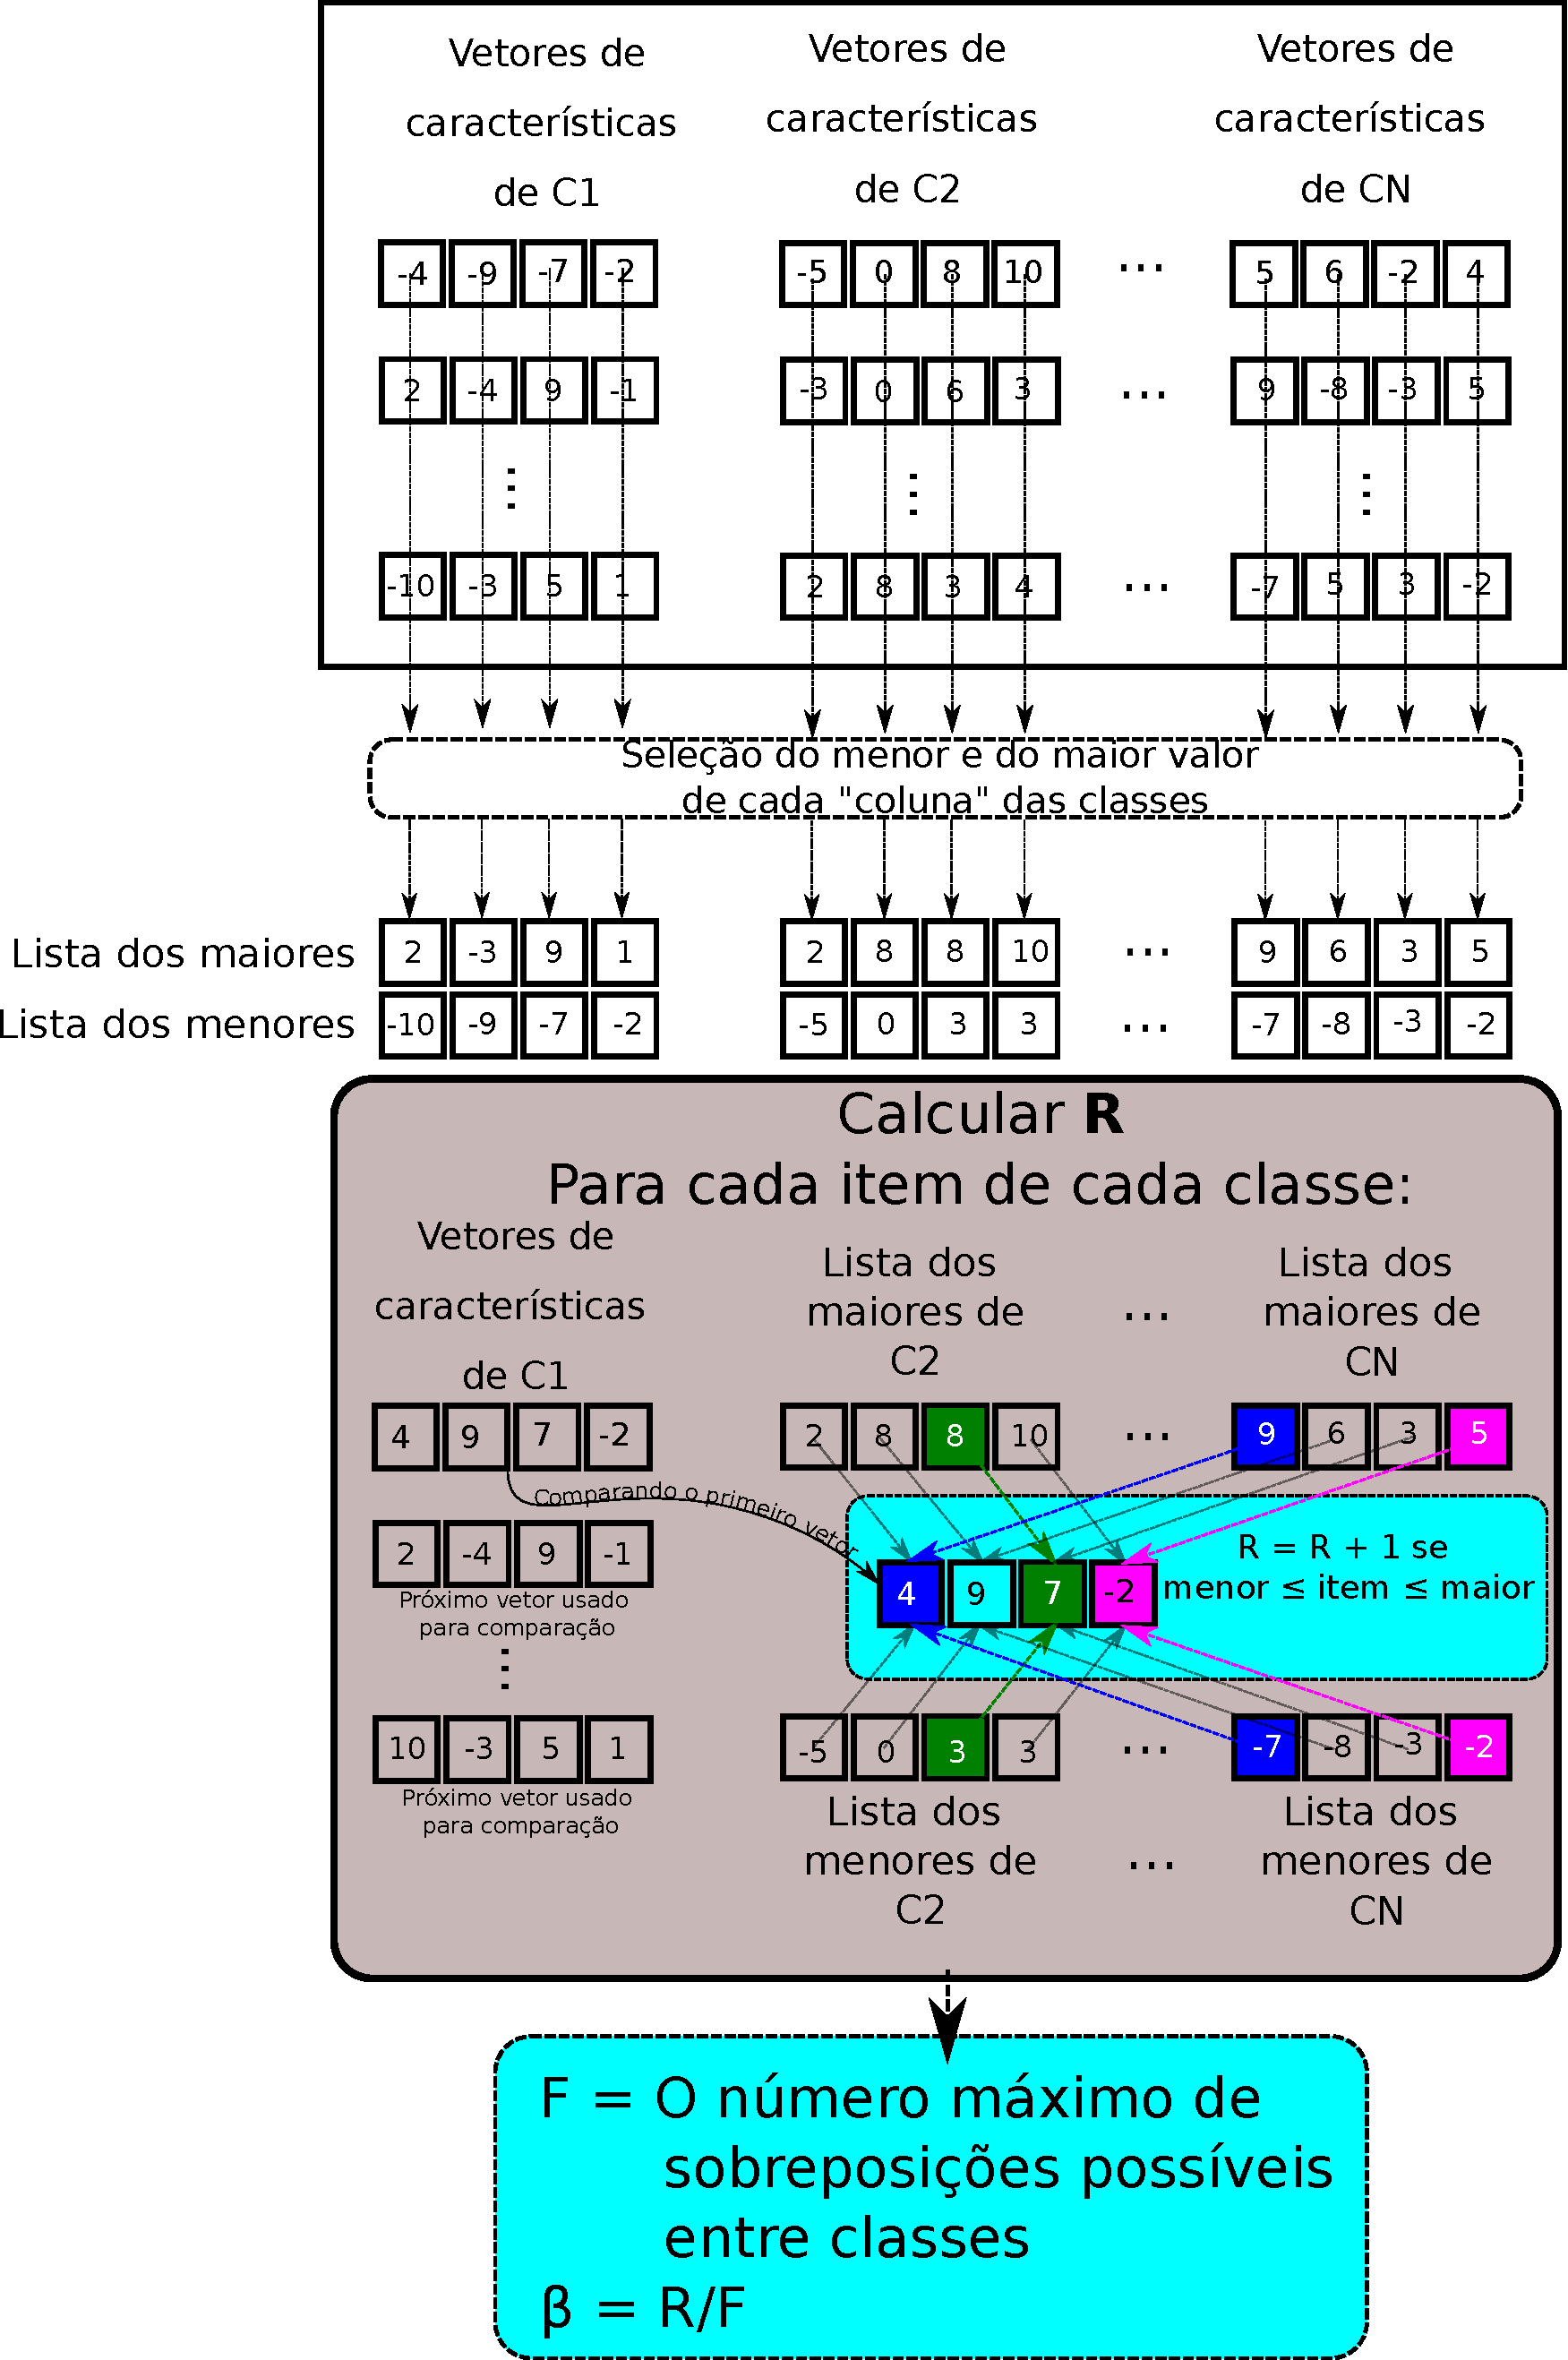
\includegraphics[width=0.77\linewidth]{images/betaCalculation.pdf}
					\label{fig:betacalculation}
					\\Fonte: Adaptado de \cite{8588433}.
				\end{figure}
				\FloatBarrier
			
				\par Considerando-se o plano paraconsistente \cite{8588433}, temos: 
				
				\begin{itemize}
					\item Verdade $\rightarrow$ fé total ($\alpha = 1$) e nenhum descrédito ($\beta = 0$)
					\item Ambiguidade $\rightarrow$ fé total ($\alpha = 1$) e descrédito total ($\beta = 1$)
					\item Falsidade $\rightarrow$ fé nula ($\alpha = 0$) e descrédito total ($\beta = 1$)
					\item Indefinição $\rightarrow$ fé nula ($\alpha = 0$) e nenhum descrédito ($\beta = 0$) \qquad.
				\end{itemize}
				
				\par No entanto, raramente $\alpha$ e $\beta$ terão valores inteiros como os mostrados na listagem acima: Na maioria das ocasiões, $0 \leqslant \alpha \leqslant 1$ e $0 \leqslant \beta \leqslant 1$. Por isso, se torna necessário o cálculo do \textbf{grau de certeza}, isto é, $G_1$, e do \textbf{grau de contradição}, isto é, $G_2$, conforme segue:
				\begin{equation}
					G_1=\alpha-\beta  \qquad,
				\end{equation}
				\begin{equation}
					G_2=\alpha+\beta-1 \qquad,
				\end{equation}
			onde: $-1 \leqslant G_1$ e  $1 \geqslant G_2$.

			\par Os valores de $G_1$ e $G_2$, em conjunto, definem os graus entre verdade ($G_1=1$) e falsidade ($G_1=-1$) e também os graus entre indefinição ($G_2=-1$) e ambiguidade ($G_2=1$). Novamente, raramente tais valores inteiros serão alcançados já que $G_1$ e $G_2$ dependem de $\alpha$ e $\beta$.
		
			\par O Plano Paraconsistente, para fins de visualização e maior rapidez na avaliação dos resultados, encontra-se ilustrado na Figura \ref{fig:paraconsistentplane} e tem quatro arestas precisamente definidas:
			\begin{itemize}
				\item (-1,0) $\rightarrow$ falsidade;
				\item (1,0) $\rightarrow$ verdade;
				\item (0,-1) $\rightarrow$ indefinição;
				\item (0,1) $\rightarrow$ ambiguidade.
			\end{itemize}
			\par A propósito de ilustração na Figura \ref{fig:paraconsistentplane}, é possível ver um pequeno círculo indicando os graus dos quatro casos listados.
	
			\par Para se ter ideia em que área exatamente se encontram as classes avaliadas, as distâncias $(D)$ do ponto $P=(G_1,G_2)$ até o limites supracitados podem ser computadas. Tais cálculos podem ser feitos da seguinte forma:

			\begin{equation}
				D_{-1,0}=\sqrt{(G_1+1)^2+(G_2)^2}\qquad,
			\end{equation}
			\begin{equation}
				D_{1,0}=\sqrt{(G_1-1)^2+(G_2)^2}\qquad,
			\end{equation}
			\begin{equation}
				D_{0,-1}=\sqrt{(G_1)^2+(G_2+1)^2}\qquad,		
			\end{equation}
			\begin{equation}
				D_{0,1}=\sqrt{(G_1)^2+(G_2-1)^2}\qquad.
			\end{equation}		

			\begin{figure}[H]
				\centering
				\caption{O plano paraconsistente: O pequeno círculo indica os graus de falsidade(-1,0), verdade(1,0), indefinição(0,-1) e ambiguidade(0,1)}
				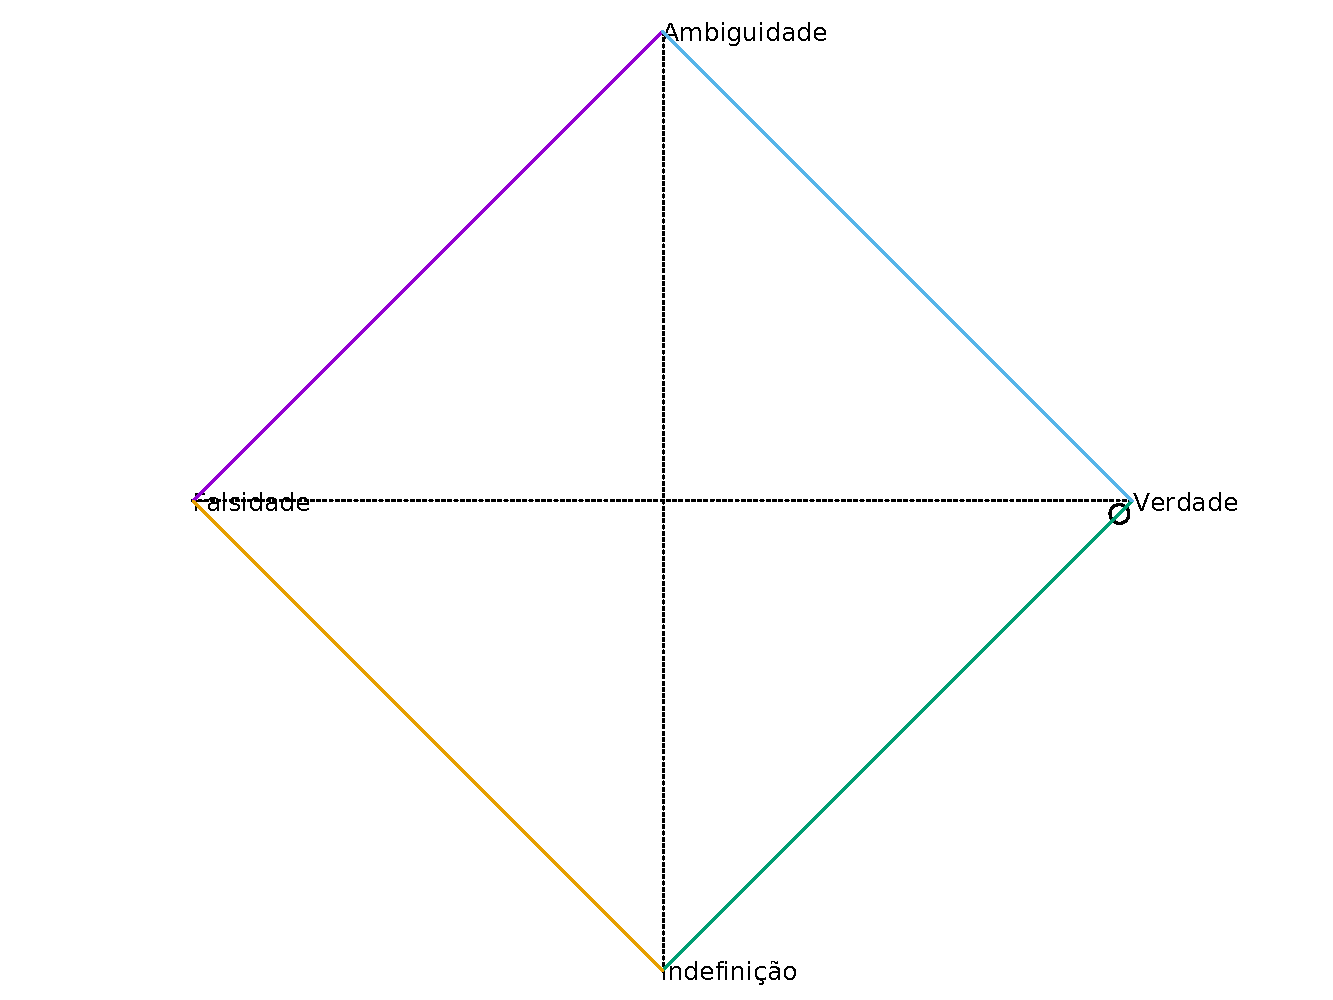
\includegraphics[angle=-90, width=0.69\linewidth]{images/paraconsistentPlane.pdf}
				\label{fig:paraconsistentplane}
				\\Fonte: Adaptado de \cite{8588433}.
			\end{figure}
		\par Na prática, ou seja, para fins de classificação, geralmente considera-se a distância em relação ao ponto \textit{``(1,0) $\rightarrow$ Verdade''}, que é o ponto ótimo: quanto mais próximo o ponto $(G_1,G_2)$ estiver de $(1,0)$, mais as os vetores de características das diferentes classes estão naturalmente separados. Isso implica a possibilidade do uso de classificadores mais modestos. 
		
	\section{Estado-da-arte em \textit{Playback Speech Detection}}
		\par No artigo \citetext{Ren2019} foi apresentado um esquema de diferenciação entre a fala comum e aquela vinda de um dispositivo reprodutor. O foco da análise se deu na distorção causada pelo alto-falante, segundo a energia e outras várias características do espectro do sinal. Uma base com 771 sinais de fala foi criada para cada um dos quatro dispositivos de gravação usados, totalizando 3084 segmentos de voz. Uma SVM foi usada como classificador. De acordo com os experimentos, a \textit{taxa de verdadeiros positivos} foi de 98,75\% e a \textit{taxa de verdadeiros negativos} foi de 98,75\%.\\
		
		\par Em \citetext{DiqunYan2019} é mostrado um método para diferenciar a voz de um locutor verdadeiro da voz gerada por sistemas usando sintetizadores baseados no \textit{modelo oculto de Markov} (HMM). SAS 2019\cite{SAS2019} foi a escolha de base de dados. Este método usa coeficientes de características logarítmicos extraídos de wavelets que são apresentados a um classificador SVM. Os resultados obtidos tiverem, em média, mais de 99\% de acurácia.\\

		\par Usando uma decomposição por espalhamento baseada em \textit{wavelets} e convertendo o resultado em coeficientes cepstrais (SCCs), o artigo \citetext{7802552} contém a descrição de um vetor de características que é avaliado por Modelos de Misturas Gaussianas (GMM) para fins de \textit{playback speech detection}. SAS 2015 \cite{SAS2015} foram as bases de dados escolhidas para os testes. Em relação aos resultados, foram usadas a \textit{taxa de falsos verdadeiros} (FAR) que representa a taxa de ocorrências falsas classificadas como verdadeiras e a \textit{taxa de falsos falsos} (FRR) que é a taxa de ocorrências verdadeiras classificadas como falsas. Os pontos em que FAR é igual a FRR foram definidos como pontos de taxa de erros iguais (ERR) e a relação $\dfrac{FAR}{FRR}$, igual a 0,18 naquele caso, foi usada como parâmetro de avaliação.\\

		\par Em \citetext{alluri2019replay}, os autores usam o \textit{zero time windowing} ou janelamento de tempo zero (ZTW) para, em conjunto com a análise cepstral do espectro gerado, fazer a análise dos sinais de voz. Os experimentos foram feitos usando-se a base SAS 2017\cite{SAS2017} com um classificador GMM e a taxa geral de ERR dos experimentos foi de 0,1475.\\
		
		\par Em \citetext{8725688}, foi registrado uma diferença entre as propriedades espectrais da voz original e da voz gravada, que pode ser expressa por meio de coeficientes cepstrais. Um GMM foi usado como classificador e a base de dados usada foi a SAS 2017. Quanto aos resultados, foi obtida uma EER geral menor que 0,1.\\
	
		\par A proposta do artigo \citetext{Hanilci2018} foi usar sinais residuais de predição linear para, juntamente com coeficientes cepstrais, criar características que foram apresentas a um classificador GMM. Novamente, a base de dados usada foi a SAS 2015 e os resultados em ERR geral foram de 5,249.\\

		\par Para detecção de \textit{playback speech}, os autores do artigo  \citetext{ISI:000473343500086} importaram, da área de processamento de imagens, o conceito de textura para o processamento de voz. Padrões binários locais (LBP) e seus respectivos histogramas foram usados para a construção do vetor de características que foi avaliado por uma SVM. A base de dados usada para testes foi a SAS 2015 e a taxa máxima de acurácia conseguida foi de 0,7167.\\
		
		\par Uma abordagem que combina análise de sinal de fala usando a \textit{Transformada Constante Q} (CQT) com o processamento cepstral foi mostrada no artigo \citetext{TODISCO2017516}. Essa técnica resulta no que se chama \textit{Coeficientes Cepstrais de Constante Q}(CQCCs). Segundo o artigo, a vantagem desses coeficientes é a resolução de espectro temporal variável. As bases de dados usadas foram a RedDots \cite{redDots}, SAS 2015 e AVSpoof 2015 \cite{AVSpoof2015}. Em se tratando de classificadores foram usados dois GMMs, cada um treinado usando os dados genuínos e \textit{spoofing} respectivamente. Os testes realizados para cada uma das bases chegou aos seguintes resultados: SAS 2015 $\rightarrow$ EER geral de 0.026; AVSpoof 2015 $\rightarrow$ EER geral de 0; RedDots $\rightarrow$ EER geral de 0,185.\\

		\par No artigo \citetext{Patel2015} é usada a \textit{Transformação Auditiva (TU)}, que tem como base a transformada \textit{wavelet}, e a \textit{Cochlear Filter Cepstral Coefficients (CFCC)} que é a junção dos métodos citados mais uma média dos valores em um intervalo de janela definido. Além disso, se define a \textit{estimação da frequência instantânea (IF)} que tem por base a Transformada de Hilbert \cite{johansson1999hilbert} e \cite{kschischang2006hilbert}. O processo todo tem como objetivo emular mecanismos naturais ocorridos dentro do ouvido e usa, além da \textit{TU}, o cálculo de coeficientes cepstrais e transformada cosseno. Para a composição dos vetores de características foram combinadas as técnicas \textit{MFCC}, \textit{CFCC}, \textit{CFCC+IF}. A base de dados usada foi a AVSpoof 2015. O classificador utilizado foi um GMM, as classificações chegaram uma EER de 0.083.\\

		\par O artigo \citetext{ISI:000490497200068} propõe uma solução para distinguir sinais de voz genuínos daqueles falseados usando reverberação e as partes não vozeadas da fala. Três GMMs foram definidos para a classificação, nesta estratégia os mesmos votam se uma ocorrência é ou não verdadeira, ganhado sempre a classificação que obtiver mais votos. A base de dados utilizada foi a  fornecida pelo \textit{``Automatic  Speaker Verification and Spoofing Contermeasures Challenge 2017''}(ASVSpoof 2017). O sistema de avaliação de desempenho escolhido, novamente, foi a ERR e esta alcançou um valor de 2,99.\\
		
		\par A principal ideia do artigo \citetext{ISI:000465363900136} foi a de capturar a amplitude instantânea vinda de flutuações de energia para distinguir entre sinais de voz genuínos daqueles falseados. Segundo os autores, as modulações de amplitude são mais suscetíveis ao ruído inserido no sinal original por uma fonte reprodutora. O estudo usa a base de dados fornecida pelo ASVSpoof 2017 e GMM como classificador. Os resultados apresentados chegaram a uma EER de 0.0019.\\

		\par No trabalho \citetext{ISI:000465363900139}, foram usadas as diferenças entre bandas de frequências específicas para diferenciar um sinal legítimo de um usado em ataques de falsificação. Particularmente, foi proposta a \textit{predição linear em domínio de frequência}(FDLP) juntamente com GMMs para classificação dos dados presentes na base  fornecida pelo ASVspoof  2017. Os resultados apresentados implicam a EER de 0.0803.\\
		
		\par No artigo \citetext{Suthokumar2018}, os autores propuseram duas novas características que visam interpretar as componentes estáticas e dinâmicas do sinal, complementando as características de tempo restrito no espectro, para distinguir entre locuções genuínas e regravadas. São elas a \textit{Modulation  Spectral Centroid Frequency} e \textit{Long Term Spectral Average}. O sistema usa como classificador um GMM juntamente com a base dados fornecida pelo ASVSpoof 2017. Os resultados mostram um valor de EER de 0,0654.\\
		
		\par Considerando o envelopamento das amplitudes e  frequências instantâneas em cada banda estreita filtrada, os autores do artigo \citetext{ISI:000458728700054} discutiram como diferenciar um sinal de voz legítimo de um falseado. A base de dados usada foi a fornecida pelo \textit{``Automatic  Speaker Verification and Spoofing Contermeasures Challenge 2015''} (ASVSpoof 2015) e o GMM foi o classificador escolhido. A proposta alcançou a EER de 0,045.\\

		\par No artigo científico \citetext{ISI:000392503100008}, foi proposto o uso do \textit{gammatone frequency cepstral coefficients}(MGFCC). O gammatone é o produto de uma distribuição gamma com um sinal senoidal e é usado na construção de filtros auditivos que, neste caso, são usados para extrair características do sinal de voz. A base de dados usada foi a fornecida pelo ASVspoof 2015 e o classificador usado foi um GMM. Na distinção entre vozes genuínas e regravadas, o EER chegou a 0,02556.\\
		
		\par Segundo o artigo \citetext{8396208}, o \textit{hashing} sensível a \textit{locus} (LSH), que é frequentemente usado como um classificador para problemas relacionados a \textit{big data}, foi combinado com coeficientes MFCCs para distinção entre locuções genuínas e regravadas. No método, os MFCCs foram extraídos dos arquivos de sinal para posterior aplicação do LSH, gerando assim uma tabela \textit{hash}. Esses valores de \textit{hash} foram então comparados, identificando assim o locutor ou locutora. Nos testes realizados houve uma acurácia de 92,66\%, a base de dados usada foi a TIMIT 2018 \cite{TIMIT2018}. \\

		\par Apesar do uso de \textit{wavelets} em alguns artigos \cite{DiqunYan2019}, \cite{Patel2015}, \cite{7802552} é interessante notar, pelo menos até o presente momento, que seu uso é escasso em técnicas de prevenção de \textit{voice spoofing}. Em uma das abordagens mais originais que usa as partes não vozeadas do sinal \cite{ISI:000490497200068}, seria muito útil o uso das transformadas \textit{wavelet} ou \textit{wavelet packet}. Tanto neste documento como em boa parte das referências utilizadas, é comum o uso de uma escala \textit{MEL} combinada com outras técnicas para construção do método de detecção de \textit{voice spoofing} \cite{Hanilci2018}, \cite{Patel2015}, \cite{8396208}, \cite{8725688}, \cite{ISI:000490497200068}. No entanto, em nenhuma dessas publicações se utilizou a escala \textit{BARK}, que foi, surpreendentemente, a que demonstrou  os melhores resultados no caso específico desta dissertação. O uso de coeficientes cepstrais combinados com outras técnicas foi muito comum \cite{alluri2019replay}, \cite{7802552}, \cite{8725688}, \cite{Hanilci2018}, \cite{TODISCO2017516}, \cite{Patel2015}, \cite{ISI:000392503100008}. Escolhidos os métodos de geração dos vetores de características, foram selecionados classificadores variados, com destaque para o relativamente simples \textit{Gaussian Mixture Models}(GMM), o mais escolhido. Este trabalho também contou com a escolha de dois classificadores modestos: Por distância Euclidiana / Manhattam e Máquina de Vetores de Suporte.\\
		
		\par A leitura dos artigos mencionados nesta seção indica ainda que, aparentemente, dentro do contexto de \textit{voice spoofing}, o esforço é para se criar vetores de características cada vez melhores, sendo curioso que em nenhum dos escritos consultados houvesse uma metodologia para comparação de resultados que não fosse a manual. Nesta dissertação, existe uma série de métodos candidatos para geração dos vetores de características baseados em \textit{wavelets} e nas escalas \textit{BARK} e \textit{MEL}. Tais candidaturas foram avaliadas segundo a engenharia paraconsistente de características que selecionou a melhor combinação dentre as opções apresentadas. Em se tratando de resultados, a maioria dos trabalhos, devido ao uso das bases \textit{SAS} e \textit{AVSpoof}, apresentaram seus resultados segundo a \textit{Equal Error Rate (EER)} que é a medida padrão para avaliação. Alguns outros utilizaram somente a acurácia \cite{8396208}, \cite{ISI:000473343500086}, \cite{DiqunYan2019}, \cite{Ren2019} e medidas calculadas em tabelas de confusão. Neste trabalho, todas as referidas métricas foram consideradas.\\

	
	\chapter{Abordagem proposta} \label{chap:propApproach}
	\section{A Base de sinais de soz}
	    \subsection{Coleta dos sinais}
		\par Para a realização desta pesquisa, coletou-se uma série de vozes nos arredores do Instituto de Biociências, Letras e Ciências Exatas da UNESP em São José do Rio Preto, no estado de São Paulo. Foram coletadas amostras de 21 indivíduos, das quais 20 foram usadas já que, em um dos casos, não foi possível coletar todos os dados necessários. Tais gravações se constituem de dígitos em um intervalo de 0 a 9 falados tanto em língua Inglesa quanto na Portuguesa. Os locutores foram escolhidos de acordo com seu sexo e idade de forma que a amostra estudada tenha uma abrangência que cubra desde crianças em época pré-escolar até adultos com idades até os 67 anos dos sexos masculino e feminino.\\
					
		\par As gravações foram realizadas usando-se um \textit{smartfone} Asus modelo \textit{Ze550kl} rodando o sistema operacional \textit{Android 6.0.1} em ambientes distintos com diferentes níveis de ruído ao fundo, garantindo uma boa variabilidade de interferências corriqueiras, caracterizando casos reais. Foram usados arquivos no formato \textit{wave}, descrito no apêndice \ref{chap:waveFile}, sem compressão com quantização de 16 bits e taxa de amostragem de 44100Hz, permitindo, segundo o teorema de Nyquist, que sejam registradas frequências de até 22050Hz.\\
		
		\par Coletados os sinais, os dígitos pronunciados nos mesmos foram separados um-a-um usando uma ferramenta desenvolvida para esse fim, resultando em um total de 410 sinais de voz de diferentes durações temporais que foram rotulados como ``genuínos''. Para cada um deles, foi criado um sinal ``espelho'',  regravado por um segundo dispositivo, um \textit{notebook} Acer modelo  \textit{Travelmate B} com o sistema operacional \textit{Arch GNU/Linux}, caracterizando os 410 sinais rotulados como ``falseados''.

	    \subsection{Organização da base de sinais}
		\par A organização da base de dados se deu por tipo, isto é, genuíno ou falseado, idioma, dígito ditado e interlocutor considerado. Foi criada uma estrutura hierárquica de diretórios de forma a permitir acesso fácil e intuitivo a cada um dos arquivos \textit{wav}, seja por vias automatizadas ou não. Os arquivos falseados residem no diretório ``playback'', enquanto que os genuínos se encontram no diretório ``live''.	Essa organização está ilustrada nas Figuras \ref{fig:directorystructlevel01}, \ref{fig:directorystructlevel02} e \ref{fig:directorystructlevel03}.\\
		
		\par Para facilitar a automatização do processamento, foram criados três arquivos de texto:
		\begin{itemize}
			\item \textit{\textbf{dataSurvey.txt}}: Contêm os dados de idade, sexo e nome do arquivo gerado para cada entrevistado;
			\item \textit{\textbf{inputListLive.txt}}: Uma lista de caminhos para todos os arquivos genuínos;
			\item \textit{\textbf{inputListSpoofing.txt}}: Apresenta uma listagem dos caminhos para todos os arquivos falseados.
		\end{itemize}
	
		\par Apenas para ilustrar, o conteúdo do diretório \textbf{``separated\textfractionsolidus live\textfractionsolidus en\_US\textfractionsolidus 0''} se constitui de vários arquivos do tipo \textit{wave}, cada um identificando o locutor ao qual pertence como exibido na Figura \ref{fig:directorystructlevel03}.

		\begin{figure}[ht]
			\centering
			\caption{Organização da base de dados}
			\subfloat[0.33\textwidth][Base em nível 1]{
				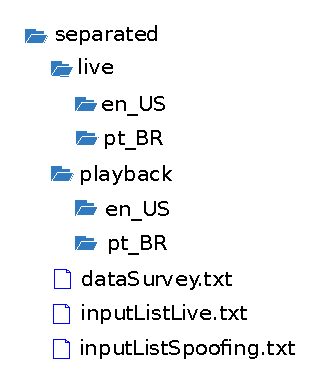
\includegraphics{images/directoryStructLevel01.pdf}
				\label{fig:directorystructlevel01}
			}
			\subfloat[0.33\textwidth][Base em nível 2]{
				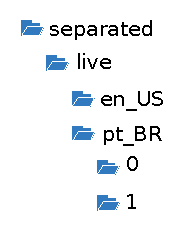
\includegraphics{images/directoryStructLevel02.pdf}
				\label{fig:directorystructlevel02}
			}
			\subfloat[0.33\textwidth][Base em nível 3]{
				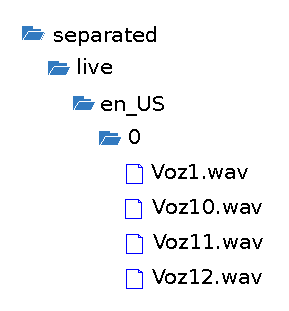
\includegraphics{images/directoryStructLevel03.pdf}
				\label{fig:directorystructlevel03}
			}
			\label{fig:directorystructlevel010203}
			\\Fonte: Elaborado pelo autor, 2021.
		\end{figure}

	\section{Estrutura da estratégia proposta}
		\par A estratégia proposta para diferenciar sinais de voz genuínos daqueles falseados deu-se conforme ilustrado na Figura \ref{fig_arq}. Particularmente, a metodologia consiste na obtenção dos dados brutos de todos os 410 + 410 = 820 sinais de voz genuínos e falseados, seguida da conversão de cada um deles para um vetor de características correspondente, conforme explicado adiante. Na sequência, os melhores sub-conjuntos de características foram escolhidos com base na Engenharia Paraconsistente. Prosseguindo, separações aleatórias entre os vetores, com proporções diversas, foram realizadas para isolar aqueles destinados ao treinamento ou modelagem do classificador utilizado dos que foram destinados aos testes de classificação. Por fim, os testes realizados e seus resultados são mostrados no Capítulo seguinte.
		
		\begin{figure}[h]
	\centering
	\caption{Estrutura da estratégia proposta}
	\scalebox{0.75}	{
		\begin{tikzpicture} 
			\node (z1)[shape=rectangle, rounded corners, draw, align=center, top color=white, bottom color=red!50] 
			at (0,2){
				\textbf{Sinal de} \\ \textbf{entrada} \\ \textbf{sob} \\ \textbf{análise}
			}; 
				
			\node (z2)[shape=rectangle, rounded corners, draw, align=center, top color=white, bottom color=yellow!50] 
			at (5.5,2){
				pré-processamento \\ e extração de \\ características no \\ domínio \textit{wavelet}
			}; 	
			
			\node (z3)[shape=rectangle, rounded corners, draw, align=center, top color=white, bottom color=yellow!50] 
			at (11,2){
				agrupamento energético \\ nas bandas Bark / Mel
			}; 	
			
			\node (z4)[shape=rectangle, rounded corners, draw, align=center, top color=white, bottom color=yellow!50] 
			at (16.5,2){
				análise paraconsistente \\ de características
			}; 
			
			\node (z5)[shape=rectangle, rounded corners, draw, align=center, top color=white, bottom color=yellow!50] 
			at (16.5,0.25){
				seleção da melhor combinação \\ agrupamento energético + wavelet
			}; 
					
			\node (z6)[shape=circle, draw, align=center, top color=white, bottom color=blue!10] 
			at (7,0.25) {};
			
			\node (z7)[shape=rectangle, rounded corners, draw, align=center, top color=white, bottom color=yellow!50] 
			at (7,-1.25) {
				classificador \\ por distâncias \\ ou SVM
			};
			
			\node (z8)[shape=rectangle, rounded corners, draw, align=center, top color=white, bottom color=green!80] 
			at (12,-1.25) {
				\textbf{Resultados}
			};
			
			\path[->] (z1) edge (z2);
			\path[->] (z2) edge (z3);
			\path[->] (z3) edge (z4);
			\path[->] (z4) edge (z5);
			\path[->] (z5) edge (z6);
			\path[->] (z6) edge (z7);	
			\path[->] (z7) edge (z8);
		\end{tikzpicture}
	}
	\label{fig_arq}
	\\Fonte: Elaborado pelo autor, 2021.
\end{figure}
		
		\par Conforme mencionado nos Capítulos anteriores, os vetores de características desta abordagem foram obtidos com base na Transformada \textit{Wavelet}, convertendo os sinais de voz do domínio do tempo para o domínio tempo-frequência. Particularmente, nos experimentos detalhados adiante, foram testados os seguintes filtros \textit{wavelet}: Haar, Daubechies de suportes 4 até 76, Symmlets com suportes 8, 16 e 32, Coiflets com suportes 6, 12, 18, 24 e 30, Beylkin com suporte 18 e, ainda, Vaidyanathan de suporte 24.

	\section{Procedimentos}
		\par De modo a garantir a comparação com outros trabalhos se fez necessário adotar várias formas de representar os resultados correspondentes para cada configuração experimental:\\
		\begin{itemize}
			\item Tabela de confusão.
			\item Acurácia e seu respectivo desvio padrão.
			\item EER (Equal Error Rate).
		\end{itemize}
		
		\par No exemplo constituído pela tabela de confusão \ref{tab:confusionMatrixSample} as \textbf{linhas} representam as \textbf{classes estimadas} e as \textbf{colunas} as \textbf{classes verdadeiras}, sendo que:
		\begin{itemize}
			\item \textbf{TP}: quantidade de itens verdadeiros classificados como tal (\textit{True Positive}).
			\item \textbf{TN}: quantidade de itens falsos classificados como tal (\textit{True Negative}).
			\item \textbf{FN}: quantidade de itens verdadeiros classificados como falsos (\textit{False Negative}).
			\item \textbf{FP}: quantidade de itens falsos classificados como verdadeiros (\textit{False Positive}).
		\end{itemize} 
		\begin{table}
\newcommand{\mc}[3]{\multicolumn{#1}{#2}{#3}}
\definecolor{tcB}{rgb}{0.447059,0.74902,0.266667}
\definecolor{tcC}{rgb}{0,0,0}
\definecolor{tcD}{rgb}{0,0.4,0.701961}
\definecolor{tcA}{rgb}{0.65098,0.65098,0.65098}
\begin{center}
	\begin{tabular}{ccc}
		% use packages: color,colortbl
		\mc{1}{l}{} & \mc{1}{>{\columncolor{tcA}}c}{\textbf{Verdadeiro}} & \mc{1}{>{\columncolor{tcA}}c}{\textbf{Falso}}\\

		\mc{1}{>{\columncolor{tcA}}r}{\textbf{Verdadeiro}} & \mc{1}{>{\columncolor{tcB}}c}{\textcolor{tcC}{VV}} & \mc{1}{>{\columncolor{tcD}}c}{\textcolor{tcC}{FV}}\\

		\mc{1}{>{\columncolor{tcA}}r}{\textbf{Falso}} & \mc{1}{>{\columncolor{tcD}}c}{\textcolor{tcC}{FF}} & \mc{1}{>{\columncolor{tcB}}c}{\textcolor{tcC}{VF}}
	\end{tabular}
	\caption{Exemplo de matriz de confusão}
	\label{tab:confusionMatrixSample}
\end{center}
\end{table}

		
		\par A acurácia usa os valores de \textit{TP}, \textit{TN} e a quantidade de elementos(\textit{N}) para ser calculada como mostrado na Equação \ref{eq:calculoDaAcuracia}.\\
		
		\begin{equation}
			acuracia = \dfrac{TP + TN}{N} \qquad.
			\label{eq:calculoDaAcuracia}
		\end{equation}

		\par Para se calcular o EER se considera os valores de \textit{FP} e \textit{FN} \cite{ghazali2018recent}, a partir desses valores são calculadas as \textit{False Acceptance Rate (\textbf{FAR})} representada na equação \ref{eq:FAR} e \textit{False Rejection Rate (\textbf{FRR})} representada por \ref{eq:FRR} ou \textbf{Taxa de falsos positivos} e \textbf{Taxa de falsos negativos} respectivamente.\\
		
		\begin{equation}
			FAR=\dfrac{FP}{TN+FP} \qquad.
			\label{eq:FAR}
		\end{equation}
		
		\begin{equation}
			FRR=\dfrac{FN}{TP+FN} \qquad.
			\label{eq:FRR}
		\end{equation}
				
		\par São calculadas tabelas de confusão por um número suficiente de vezes até que \textbf{\textit{FAR} seja igual \textit{FRR}}, a cada ciclo os vetores de características são comutados de forma aleatória para que se consiga valores diferentes, neste trabalho alguns casos precisaram de mais que 12000 iterações para que se encontrasse uma configuração em que FAR=FRR.\\
		
		\par Em cada iteração os valores de FAR e FRR são guardados em dois vetores, um para cada, então o vetor pertencente a FAR é ordenado de forma crescente e o outro decrescente. Esses pontos desenhados no gráfico com uma linha que divide o plano do mesmo ao meio tal que $x=y$ constituem o que se convencionou chamar de gráfico de \textit{Detection Error Tradeoff (DET)} ou, em tradução livre, \textbf{gráfico para balanceamento de erros}.\\
		
		\par O efetivo valor de \textbf{ERR se encontra na intersecção da reta $x=y$} com a curva definida por FAR e FRR, por isso o cálculo de um valor único como demonstrado no Algoritmo \ref{lst:EERAlgo} e na Figura \ref{fig:eeralgo} pois se $x=ERR$ então também $y=ERR$.\\\\
	
		\begin{lstlisting}[language=C++, caption={EER algorithm}, label={lst:EERAlgo}]
double shortestDistance = highestValue();
double currentDistance = -highestValue();

double coordinateAboveDiagonalLine = { 0, 0 };
double coordinateBellowDiagonalLine = { 0, 0 };

sortAscending(FARVector);
sortDescending(FRRVector);

for (i = 0; i < FARVector.size(); i++) {
	// Calculate the distance between the coordinates defined
	// by the FAR and FRR vectors and the line defined by x=y
	currentDistance = absoluteValue((FARVector[i] - FRRVector[i]) / squaredRoot(2));
	
	// Stores just the shortest distance above the x=y line
	if (currentDistance <= shortestDistance && FRRVector[i] >= FARVector[i]) {
		shortestDistance = currentDistance;
		coordinateAboveDiagonalLine[0] = FARVector[i];
		coordinateAboveDiagonalLine[1] = FRRVector[i];
		jumpToNextIteration();
	}

	// Stores just the shortest distance bellow the x=y line
	coordinateBellowDiagonalLine[0] = FARVector[i];
	coordinateBellowDiagonalLine[1] = FRRVector[i];
	
	breakLoop();
}

// Calculates the intersection point of the curve defined by the FAR and FRR points and the x=y line
y = coordinateAboveDiagonalLine[0] - coordinateBellowDiagonalLine[0] - 1;
x = coordinateBellowDiagonalLine[1] - coordinateAboveDiagonalLine[1] + 1;
c = coordinateAboveDiagonalLine[1] * coordinateBellowDiagonalLine[0] - coordinateAboveDiagonalLine[0] * coordinateBellowDiagonalLine[1];

// Calculates the equal error rate
EER = -(c / (x + y));
\end{lstlisting}

		\begin{figure}[H]
			\centering
			\caption{Algoritmo para o cálculo do EER}
			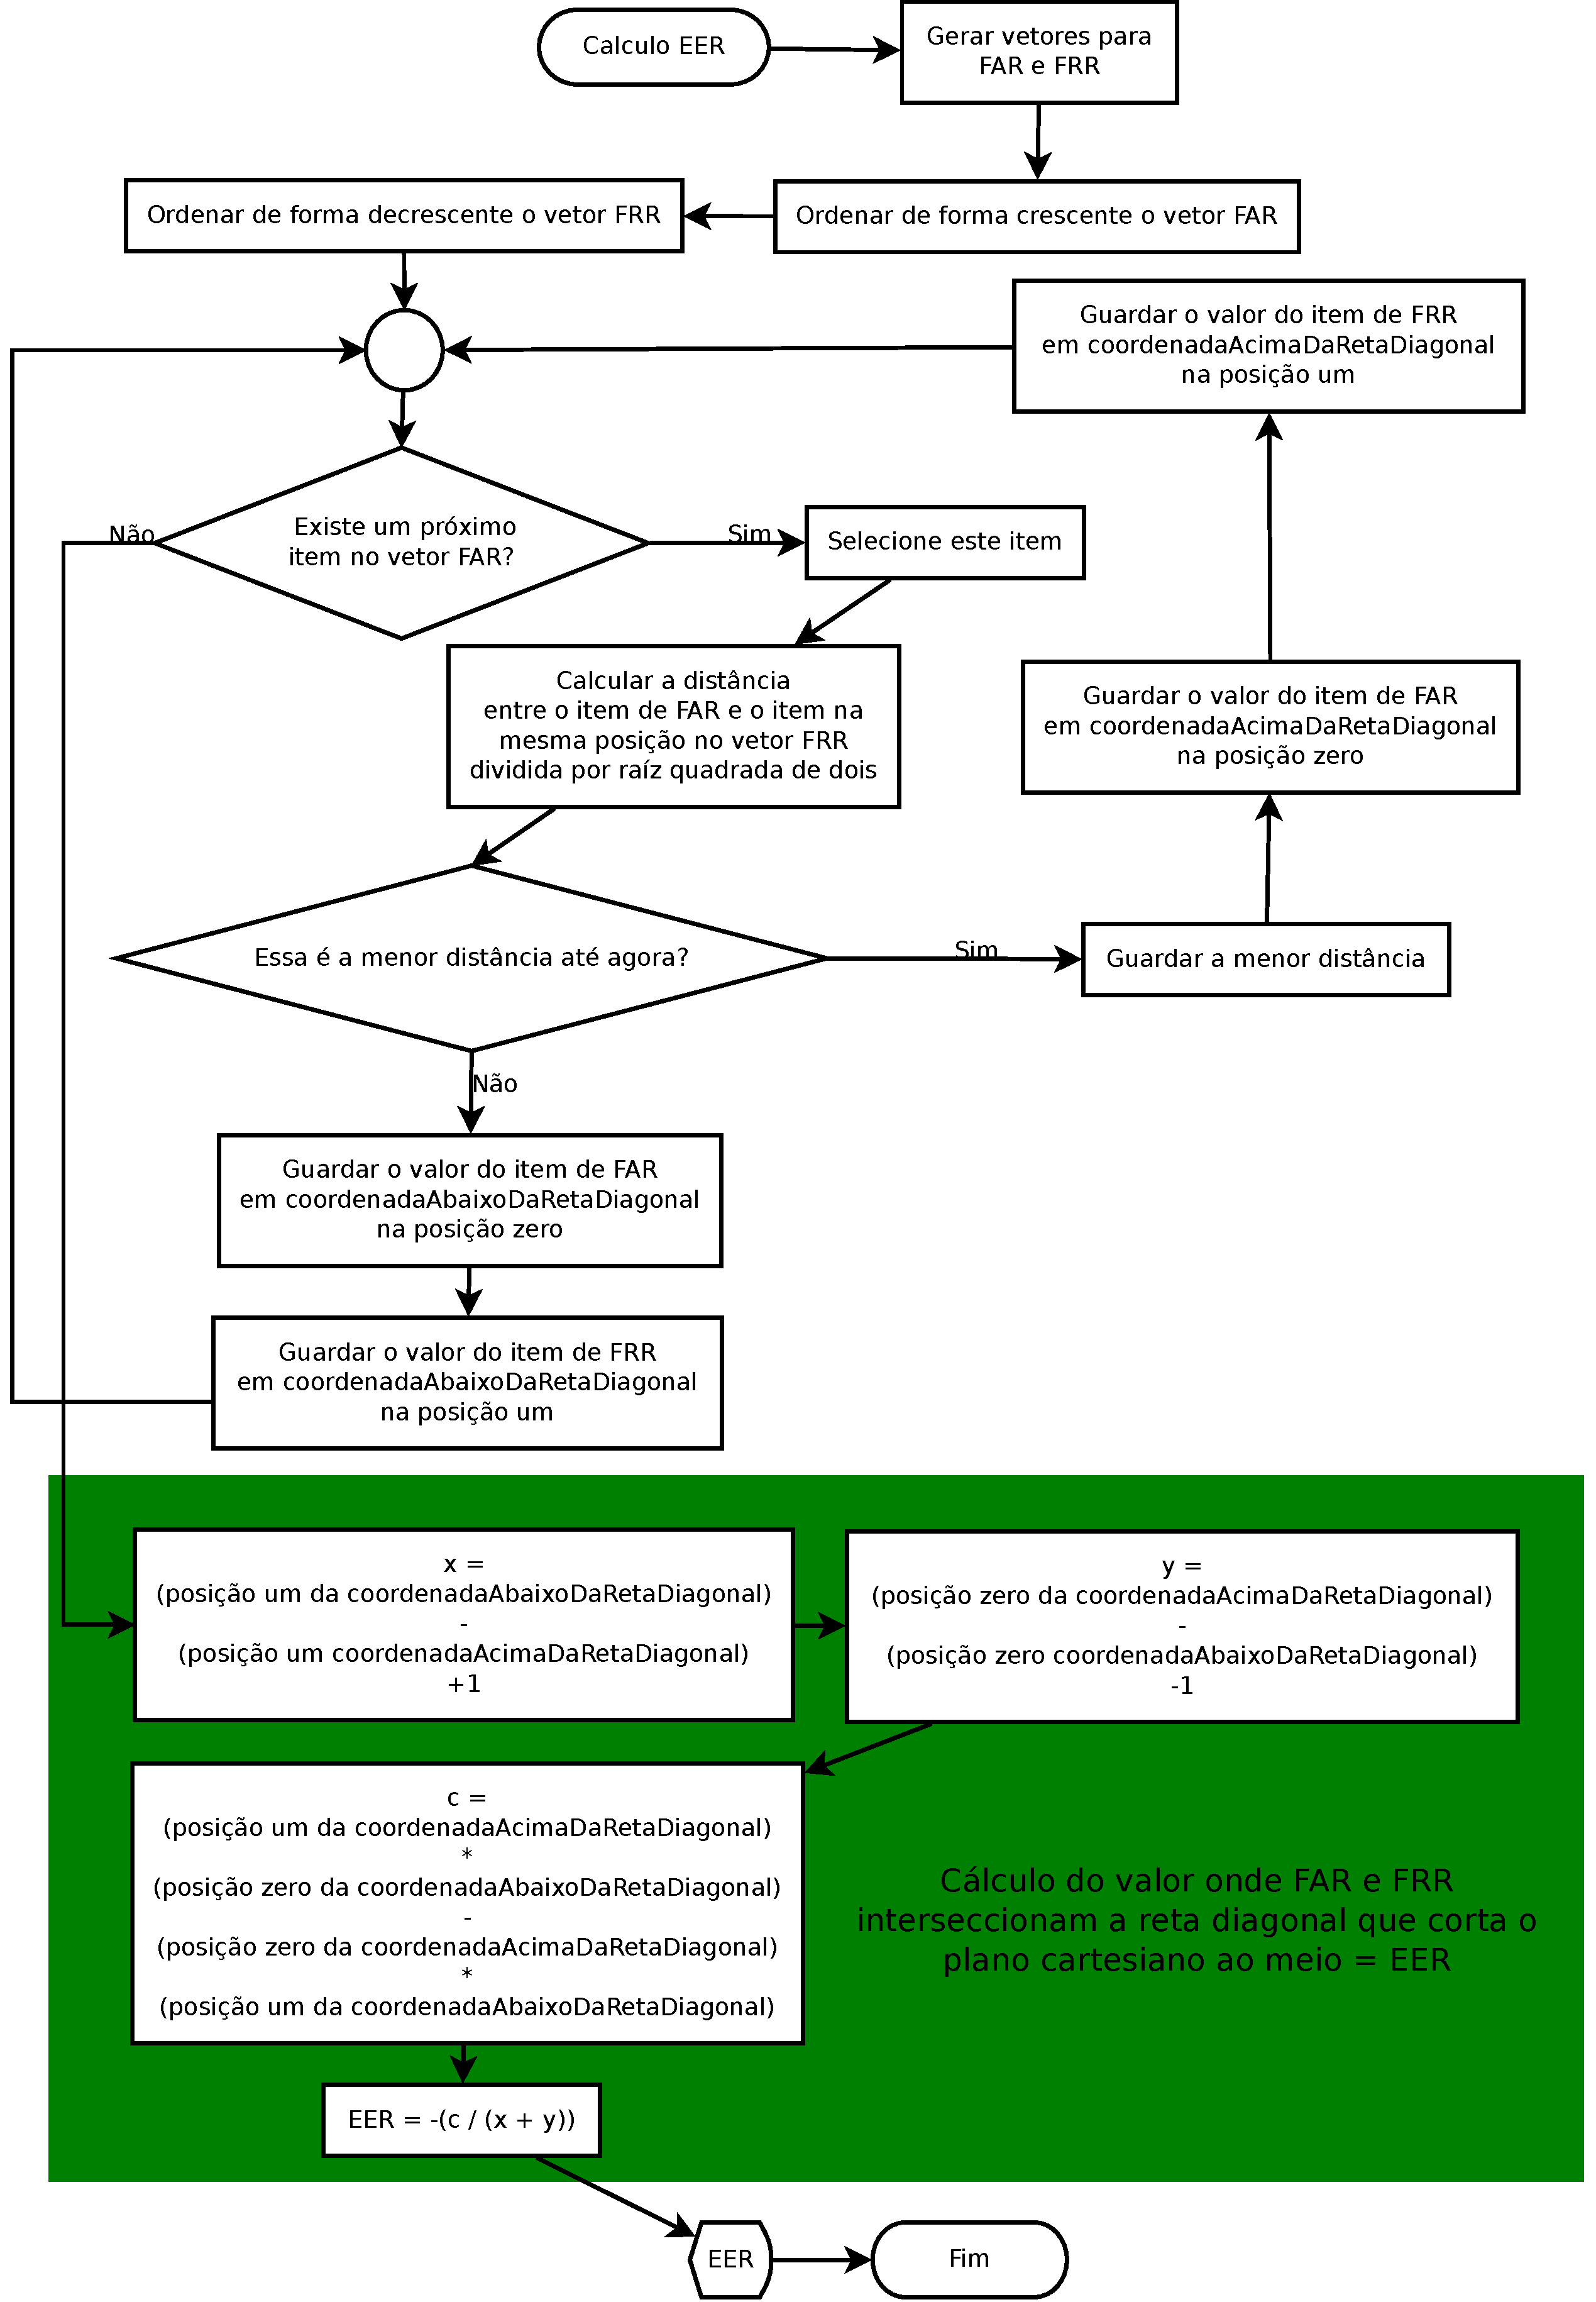
\includegraphics[width=1\linewidth]{images/EERAlgo.pdf}
			\label{fig:eeralgo}
			\\Fonte: Elaborado pelo autor, 2021.
		\end{figure}
	
		\subsection{Procedimento 01: Filtros \textit{wavelet}, escalas Bark e Mel}
		\label{chap:propApproach:sec:Experimento01}
		\par O objetivo deste procedimento é o de verificar, segundo a Engenharia Paraconsistente, qual das combinações entre as escalas BARK ou MEL e as várias \textit{wavelets} consideradas geram os vetores de características mais propícios, ou seja, que atraem o ponto $(G_1,G_2)$ para uma posição mais próxima do vértice $(1,0)$ do plano paraconsistente, conforme mencionado no Capítulo anterior. \\
				
		\par As transformações \textit{wavelet-packet} foram realizadas, com os diversos filtros mencionados, até  o máximo nível possível, implicando máxima resolução em frequência para que, após isso, as amostras dos sinais transformados fossem agrupadas visando corresponder aos intervalos espectrais definidos nas escalas BARK e MEL. Naquela escala, os vetores de características foram constituídos de 24 coeficientes, diferentemente, nesta escala, os vetores de características foram formados com 13 coeficientes devido à derivação do sinal ao final do processo de geração. O Algoritmo \ref{lst:experiment01Algo} e Figura \ref{fig:experiment01Algo} contém a descrição de tais procedimentos.\\

		\begin{lstlisting}[language=C++]
// Carregue para a memoria um dos conjuntos de amostra
for (listaDeAmostras : {listaComVoiceSpoofing, listaSemVoiceSpoofing}) {
	// Selecione o proximo tipo de wavelet
	for (wavelet : wavelets) {
		// Selecione entre BARK ou MEL
		for (barkOuMel : {BARK, MEL}) {
			// Selecione o proximo sinal dentro da amostra
			for (sinal : listaDeAmostras) {
				tamanhoOtimo=calcularTamanhoOtimo(sinal);
				redimensionar(sinal, tamanhoOtimo);
				sinalTransformado=wavelet(sinal, wavelet);
				energias=calcularEnergias(sinalTransformado, barkOuMel);
				energias=normalizar(energias);
				
				// Armazene os resultados
				resultados[wavelet.nome()][barkOuMel][listaDeAmostras.nome()].adicionar(energias);
			}
		}
	}
}
// Posicione os resultados no plano paraconsistente
mostraResultadosNoPlanoParaconsistente(resultados);
\end{lstlisting}
			
		\begin{figure}[H]
			\centering
			\caption{Algoritmo que caracteriza o Procedimento 01}
			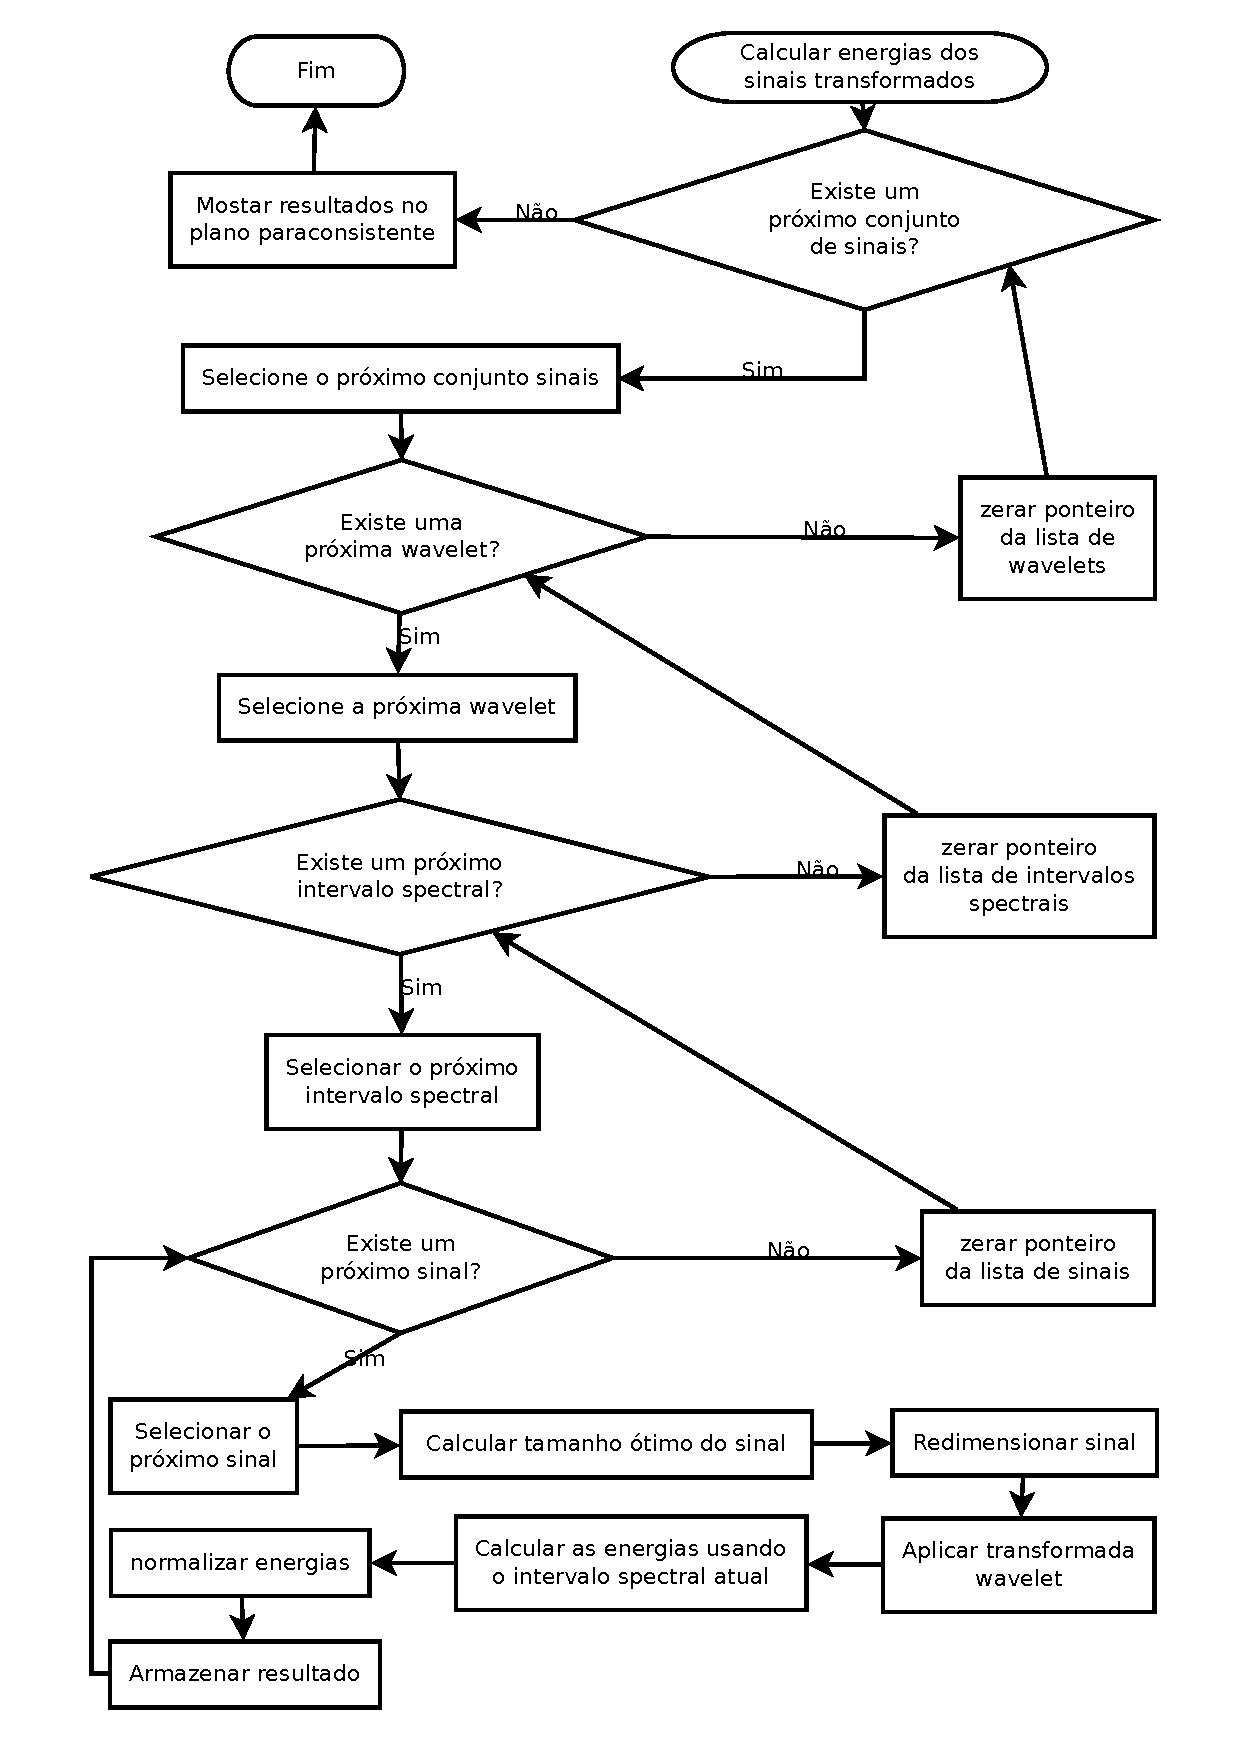
\includegraphics[width=1\linewidth]{images/AlgoProcedure01.pdf}
			\label{fig:experiment01Algo}
			\\Fonte: Elaborado pelo autor, 2021.
		\end{figure}
		
		\par Registre-se que, antes da aplicação da transformada \textit{wavelet-packet}, foi necessária uma normalização de valores do sinal entre os intervalos -1 e 1 seguida de um redimensionamento para que houvesse um comprimento correspondente a uma potência de 2, como indicado na equação \ref{eq:optimalSize}. Isso é necessário para que não haja perdas de trechos de voz ao final da transformação, pois a transformada \textit{wavelet} realiza um \textit{downsampling} de ordem 2, ou seja, em cada nível de decomposição o tamanho do vetor do sinal é diminuído pela metade. Caso haja um comprimento diferente do citado, em alguma parte do processo a divisão não será inteira fazendo com que algumas amostras dos sinais sejam perdidas.
				
		\par Para ajustar o tamanho do sinal de voz sob análise, foi usada a Equação \ref{eq:optimalSize}, na qual \textit{\textbf{proxInt}} é uma função que retorna o próximo número inteiro do argumento real. Por exemplo, $proxInt(1,5) = 2$.

		\begin{equation}
			tamanhoOtimo=2^{proxInt(\log_{2}tamanho)}
			\label{eq:optimalSize}
		\end{equation} 
		
		\par Após o redimensionamento do tamanho do sinal, o nível máximo de transformações é dado pela Equação \ref{eq:maxWaveletTransf}. 
				
		\begin{equation}
			maxTrans=\log_{2}(tamanhoOtimo) \qquad.
			\label{eq:maxWaveletTransf}
		\end{equation}
		
		\subsection{Procedimento 02 - Classificações baseadas em distâncias}
		\label{chap:propApproach:sec:Experimento02}
		\par O objetivo deste procedimento é verificar, considerando as melhores combinações descobertas pelo procedimento anterior, a acurácia de classificadores \textit{pattern-matching} por distâncias Euclidiana e Manhattan. Nesta fase, os vetores de características gerados pelo Procedimento 01 são fornecidos aos classificadores para as mensurações devidas.
				
		\par Objetivando avaliar o comportamento dos classificadores com proporções múltiplas de 10\% da base de dados reservadas para modelagem até o limite de 50\%, e o restante para testes, definiu-se que, para cada proporção, o sorteio aleatório para escolha dos vetores de características e o treinamento dos classificadores seria executado $n=t \cdot \frac{t+1}{2}$ vezes, sendo $t$ o número máximo de testes que podem ser realizados com uma certa porcentagem dos vetores, em outras palavras, \textbf{a cada ciclo de treinamento e classificação os vetores nas amostras falseadas e genuínas foram sorteados aleatoriamente de acordo com a porcentagem vigente.}
				
		\par Para cada porcentagem foram coletadas as melhores e as piores acurácias assim como suas respectivas matrizes de confusão, e assim, calculadas suas \textit{EERs} conforme consta no Capítulo seguinte. No Algoritmo \ref{lst:experiment02Algo} e na Figura \ref{fig:experiment02Algo}, os passos estão detalhados.
		
		\par Essencialmente, este Procedimento 02 consiste em mensurar as distâncias entre cada vetor de características isolado para testes em relação à cada um dos vetores de características isolados para a modelagem, selecionando-se a menor delas. Em seguida, classifica-se o vetor de características que pertence aos testes e está sob análise, como pertencente a uma das classes dos vetores de modelagem selecionados.   

		\begin{figure}[H]
			\centering
			\caption{Algoritmo que caracteriza o Procedimento 02}
			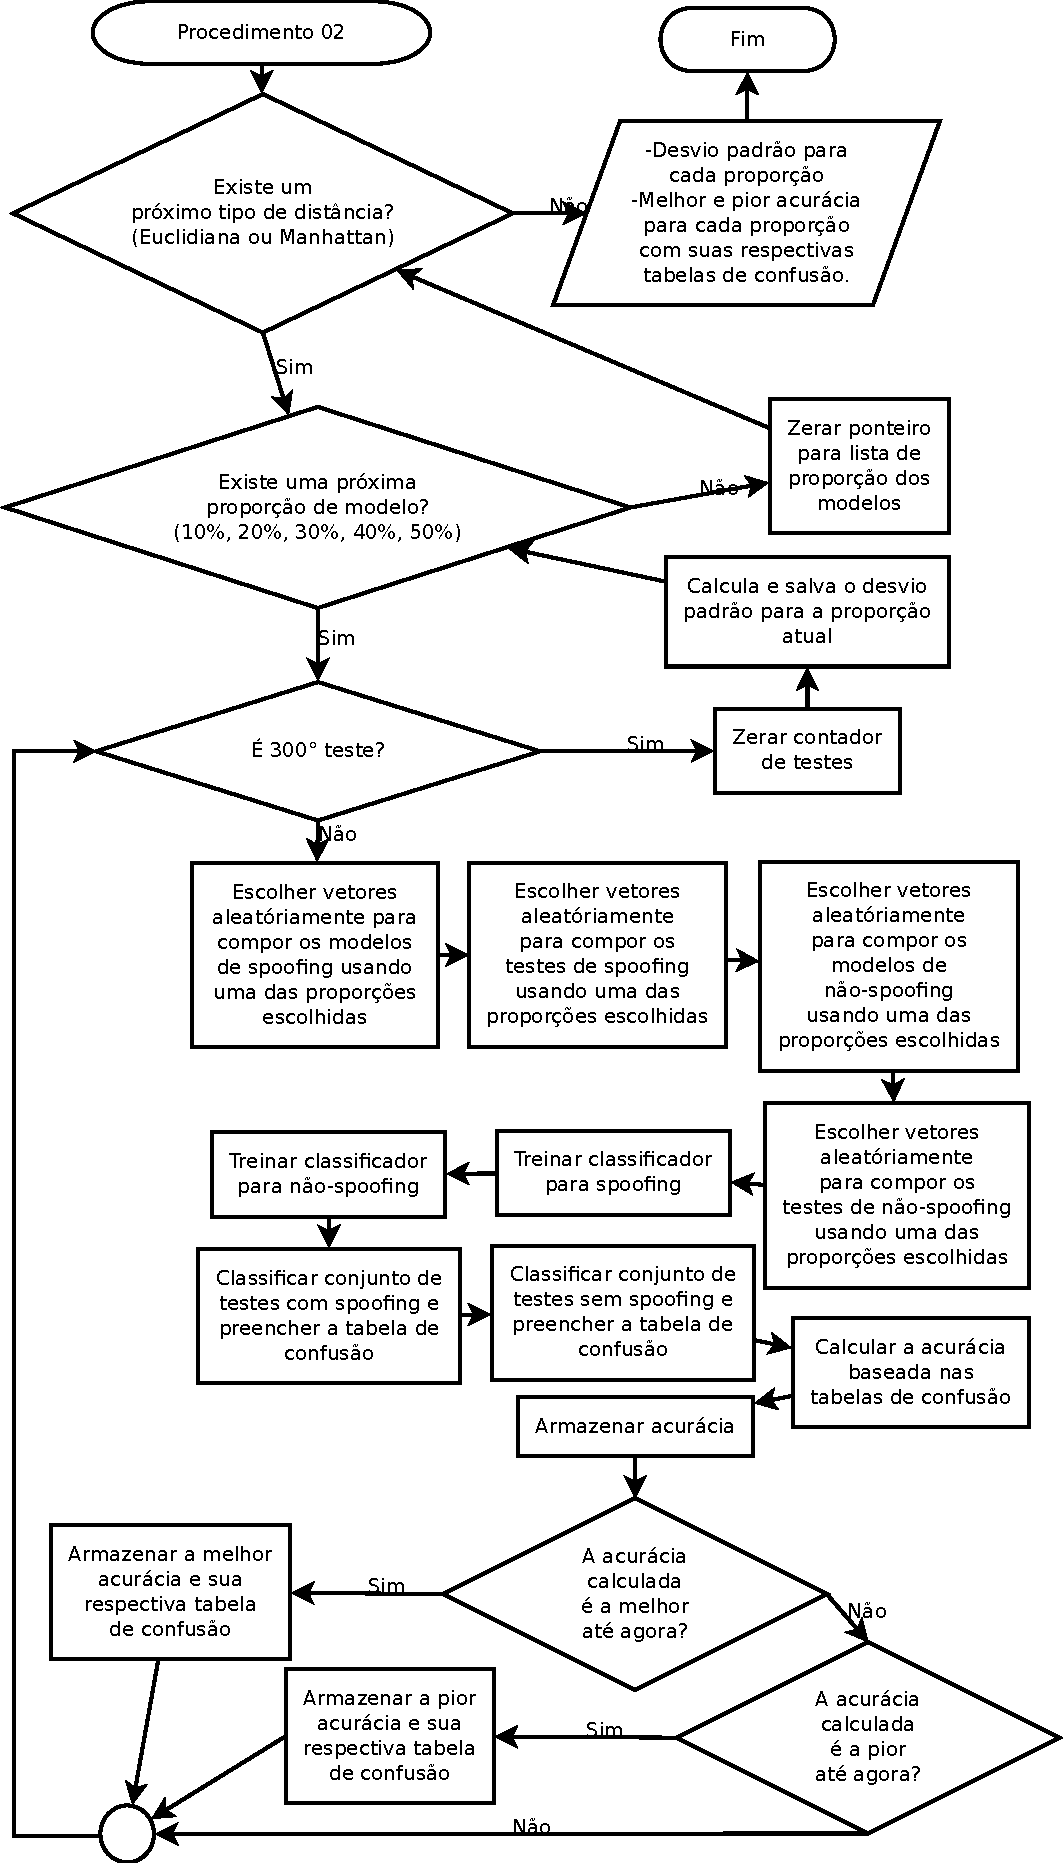
\includegraphics[width=.75\linewidth]{images/AlgoProcedure02}
			\label{fig:experiment02Algo}
			\\Fonte: Elaborado pelo autor, 2021.
		\end{figure}
		
		\begin{lstlisting}[language=C++, caption={Procedure 02 algorithm}, label={lst:experiment02Algo}]
modelProportion={0.1, 0,2, 0,4, 0,5};
genuineModel = spoofingModel= genuineTest = spoofingTest = accuracyList = {};
for (distance : {Euclidian, Manhattan}) {
	for(percentage : modelProportion){
		for(testCounter = 0; testCounter < 300; testCounter++){
			// Choose feature vectors randomly from spoofing set
			// to build the model according to the proportions chosen.
			chooseRamdomly(voiceSpoofingSet, percentage, spoofingModel, spoofingTest);
			// Choose feature vectors randomly from genuine set
			// to build the tests according to the proportion chosen
			chooseRamdomly(genuineSet, percentage, genuineModel, genuineTest);
			
			trainClassificator("spoofing", spoofingModel);
			trainClassificator("genuine", genuineModel);
			// Classify the spoofing tests against the 
			// spoofing model and fill the confusion tables
			for(signal : spoofingTest){
				fillConfusionTable(signal, "spoofing");
			} 
			// Classify the genuine tests against the
			// genuine model and fill the confusion tables
			for(signal : genuineTest){
				fillConfusionTable(signal, "genuine");
			}

			accuracy=calculateAccuracy();
			
			// Store the accuracies for each percentage
			accuracyList[percentage].add(accuracy);

			// Store the best accuracy and its respective confusion table
			if(isTheBestAccuracy(accuracy)){
				saveAccuracyAndItsConfusionTable();
			}
			
			// Store the worst accuracy and its respective confusion table
			if(isTheWorstAccuracy(accuracy)){
				saveAccuracyAndItsConfusionTable();
			}
		}
		
		// Calculate and save the standard deviation for current proportion
		calculateAndSaveTheStandardDeviation(accuracyList[percentage]);
	}
}				
\end{lstlisting}

		\subsection{Procedimento 03 - classificações baseadas na SVM}
		\label{chap:propApproach:sec:Experimento03}
		\par Considerando as melhores combinações descobertas durante o Procedimento 01, esta etapa visa medir a acurácia de uma SVM na separação das classes. O referido classificador foi escolhido, pois, estudos anteriores comprovam a sua eficácia para classificação binária \cite{bennett2000support}. \\
		
		\par Particularmente, a estrutura da SVM utilizada foi definida da seguinte forma e de acordo com a Figura \ref{fig:3layersSVM}: 
		\begin{itemize}
			\item três camadas, sendo a primeira de entrada, com elementos passivos, a segunda com elementos ativos não-lineares de núcleos Gaussianos e a terceira, isto é, a de saída, com um elemento ativo linear; 
			
			\item inexistem pesos entre a camada de entrada e a camada intermediária, implicando que a saída de cada elemento da camada de entrada conecta-se com todas as entradas de cada elemento da camada intermediária, mantendo incólumes os valores propagados;

			\item a saída de cada elemento da camada intermediária conecta-se com o único elemento da camada de saída por meio dos pesos $p_0, p_1, .... p_{X-1}$;

			\item o valor de saída consiste na combinação linear dos pesos com os valores recebidos como entrada da camada de saída, isto é, os valores de saída da camada intermediária.
		\end{itemize}

		\begin{figure}
	\centering
	\scalebox{2}{
				\begin{tikzpicture}
	%input layer
	\node (input1) at (0.65,2.0) {};
	\draw[->,in=180,out=0] (1.0,2.0) to (1.35,2.0);
	\node (input2) at (0.65,1.5) {};
	\draw[->,in=180,out=0] (1.0,1.5) to (1.35,1.5);
	\node (input3) at (0.65,1.0) {};
	\draw[->,in=180,out=0] (1.0,1.0) to (1.35,1.0);
	\node (input3) at (0.65,0.0) {};
	\draw[->,in=180,out=0] (1.0,0.0) to (1.35,0.0);
	\node (IL_N1) at (1.5,2.0) {}; \filldraw[fill=gray!30] (1.5,2.0) circle (0.15cm);
	\node (IL_N2) at (1.5,1.5) {}; \filldraw[fill=gray!30] (1.5,1.5) circle (0.15cm);
	\node (IL_N3) at (1.5,1.0) {}; \filldraw[fill=gray!30] (1.5,1.0) circle (0.15cm);
	\node at (1.5,0.625) {$\vdots$};
	\node (IL_Nn) at (1.5,0.0) {}; \filldraw[fill=gray!30] (1.5,0.0) circle (0.15cm);
	
	%hidden layer 
	\node (HL_N1) at (3.5,2.5) {}; \filldraw[fill=blue!20] (3.55,2.5) circle (0.15cm);
	\node (HL_N2) at (3.5,2.0) {}; \filldraw[fill=blue!20] (3.55,2.0) circle (0.15cm);
	\node (HL_N3) at (3.5,1.5) {}; \filldraw[fill=blue!20] (3.55,1.5) circle (0.15cm);
	\node (HL_N4) at (3.5,1.0) {}; \filldraw[fill=blue!20] (3.55,1.0) circle (0.15cm);
	\node at (3.55,0.625) {$\vdots$};
	\node (HL_Nn-1) at (3.5,0.0) {}; \filldraw[fill=blue!20] (3.55,0.0) circle (0.15cm);	
	\node (HL_Nn) at (3.5,-0.5) {}; \filldraw[fill=blue!20] (3.55,-0.5) circle (0.15cm);	
	\draw[->,in=180,out=0] (IL_N1)+(1.5mm,0) to (HL_N1);
	\draw[->,in=180,out=0] (IL_N1)+(1.5mm,0) to (HL_N2);
	\draw[->,in=180,out=0] (IL_N1)+(1.5mm,0) to (HL_N3);
	\draw[->,in=180,out=0] (IL_N1)+(1.5mm,0) to (HL_N4);
	\draw[->,in=180,out=0] (IL_N1)+(1.5mm,0) to (HL_Nn-1);
	\draw[->,in=180,out=0] (IL_N1)+(1.5mm,0) to (HL_Nn);
	
	\draw[->,in=180,out=0] (IL_N2)+(1.5mm,0) to (HL_N1);
	\draw[->,in=180,out=0] (IL_N2)+(1.5mm,0) to (HL_N2);
	\draw[->,in=180,out=0] (IL_N2)+(1.5mm,0) to (HL_N3);
	\draw[->,in=180,out=0] (IL_N2)+(1.5mm,0) to (HL_N4);
	\draw[->,in=180,out=0] (IL_N2)+(1.5mm,0) to (HL_Nn-1);
	\draw[->,in=180,out=0] (IL_N2)+(1.5mm,0) to (HL_Nn);
	
	\draw[->,in=180,out=0] (IL_N3)+(1.5mm,0) to (HL_N1);
	\draw[->,in=180,out=0] (IL_N3)+(1.5mm,0) to (HL_N2);
	\draw[->,in=180,out=0] (IL_N3)+(1.5mm,0) to (HL_N3);
	\draw[->,in=180,out=0] (IL_N3)+(1.5mm,0) to (HL_N4);
	\draw[->,in=180,out=0] (IL_N3)+(1.5mm,0) to (HL_Nn-1);
	\draw[->,in=180,out=0] (IL_N3)+(1.5mm,0) to (HL_Nn);
	
	\draw[->,in=180,out=0] (IL_Nn)+(1.5mm,0) to (HL_N1);
	\draw[->,in=180,out=0] (IL_Nn)+(1.5mm,0) to (HL_N2);
	\draw[->,in=180,out=0] (IL_Nn)+(1.5mm,0) to (HL_N3);
	\draw[->,in=180,out=0] (IL_Nn)+(1.5mm,0) to (HL_N4);
	\draw[->,in=180,out=0] (IL_Nn)+(1.5mm,0) to (HL_Nn-1);
	\draw[->,in=180,out=0] (IL_Nn)+(1.5mm,0) to (HL_Nn);
	
	%output layer
	\node (OL_N1) at (5.5,1.0) {}; \filldraw[fill=red!40] (5.55,1.0) circle (0.15cm);
	
	\draw[->,in=180,out=0] (HL_N1)+(2mm,0) to (OL_N1);
	\draw[->,in=180,out=0] (HL_N2)+(2mm,0) to (OL_N1);
	\draw[->,in=180,out=0] (HL_N3)+(2mm,0) to (OL_N1);
	\draw[->,in=180,out=0] (HL_N4)+(2mm,0) to (OL_N1);
	\draw[->,in=180,out=0] (HL_Nn-1)+(2mm,0) to (OL_N1);
	\draw[->,in=180,out=0] (HL_Nn)+(2mm,0) to (OL_N1);
	%
	\draw[snake=brace,mirror snake,raise snake=45pt,brown] (1.25,1.25) -- (1.75,1.25) node[black,midway,yshift=-50pt,below]{\tiny camada de} node[black,midway,yshift=-58pt,below]{\tiny entrada com} node[black,midway,yshift=-66pt,below]{\tiny $R$ elementos}
	node[black,midway,yshift=-74pt,below]{\tiny passivos};
	\draw[snake=brace,mirror snake,raise snake=45pt,brown] (3.25,0.75) -- (3.75,0.75) node[black,midway,yshift=-50pt,below]{\tiny camada} node[black,midway,yshift=-58pt,below]{\tiny intermediária} node[black,midway,yshift=-66pt,below]{\tiny com $X$ neurônios}
	node[black,midway,yshift=-74pt,below]{\tiny ativos não-lineares};
	\draw[snake=brace,mirror snake,raise snake=45pt,brown] (5.25,1.75) -- (5.75,1.75) node[black,midway,yshift=-50pt,below]{\tiny camada de} node[black,midway,yshift=-58pt,below]{\tiny saída com} node[black,midway,yshift=-66pt,below]{\tiny um elemento}
	node[black,midway,yshift=-74pt,below]{\tiny ativo linear};
	%
	\node (OUT) at (6.5,1.0) {\tiny resultado}; 
	\draw[->,in=180,out=0] (OL_N1)+(2mm,0) to (OUT);	
	
	\node at (4,2.6) {\tiny $p_0$}; 
	\node at (4,2.1) {\tiny $p_1$}; 
	\node at (4,1.65) {\tiny $p_2$}; 
	\node at (4,1.2) {\tiny $p_3$}; 
	\node at (4,0.2) {\tiny $p_{X-2}$}; 
	\node at (4,-0.3) {\tiny $p_{X-1}$}; 
\end{tikzpicture}
	}
	\caption{Estrutura da SVM para o procedimento 03 com $R$ neurônios na camada de entrada, sendo $R$ a dimensão dos vetores de características, e $X$ neurônios na camada intermediária, sendo $X$ o número de casos de treinamento}
	\label{fig:3layersSVM}
\end{figure} 

		\par Foram utilizados, na camada de entrada, um número de elementos igual a dimensão do vetor de características sendo considerado. Na camada intermediária, o número de elementos ativos não-lineares foi igual ao número de casos de treinamento, visando facilitar o procedimento que, em tal caso, implica na solução direta de um sistema linear quadrado, isto é, possível e determinado \cite{poole2014linear}.\\
		
		\par O treinamento da SVM consiste em, numa primeira etapa não-supervisionada, ajustar os parâmetros das funções Gaussianas da camada intermediária. Posteriormente, com base no sistema linear mencionado, os pesos foram encontrados com base em uma abordagem supervisionada, utilizando-se os rótulos -1 e 1 para os sinais falseados e genuínos, respectivamente.
		
		\par Todos os arranjos para a seleção dos vetores de treinamento e testes, assim como demais detalhes,   são idênticos àqueles do procedimento 02 e encontram-se listados no Algoritmo \ref{lst:experiment03Algo} e na Figura \ref{fig:experiment03Algo}.\\
		
		\begin{lstlisting}[language=C++, caption={Algoritmo que caracteriza o procedimento 03}, label={lst:experiment03Algo}]
tamanhosDoModelo={0.1, 0,2, 0,4, 0,5};
modeloDeReferenciaNaoSpoofing={};
modeloDeReferenciaSpoofing={};
testesNaoSpoofing={};
testesSpoofing={};
	for(porcentagem : tamanhosDoModelo){
		for(teste = 0; teste < 300; teste++){
			// Escolhe aleatoriamente os sinais para o modelo com spoofing 
			// e os grava em 'modeloDeReferenciaSpoofing' o restante vai 
			// para 'testesSpoofing'
			escolherAleatoriamente(listaComVoiceSpoofing, porcentagem, modeloDeReferenciaSpoofing, testesSpoofing);
			
			// Escolhe aleatoriamente os sinais para o modelo sem spoofing
			// e os grava em 'modeloDeReferenciaNaoSpoofing' o restante vai 
			// para 'testesNaoSpoofing'
			escolherAleatoriamente(listaSemVoiceSpoofing, porcentagem, modeloDeReferenciaNaoSpoofing, testesNaoSpoofing);
			treinarClassificador("spoofing", modeloDeReferenciaSpoofing);
			treinarClassificador("naoSpoofing", modeloDeReferenciaNaoSpoofing);
			
			// Classifica os testes e preenche a tabela de confusao
			for(sinal : testesSpoofing){
				preencherTabelaDeConfusao(sinal, "spoofing");
			} 
			
			// Classifica os testes e preenche a tabela de confusao
			for(sinal : testesNaoSpoofing){
				preencherTabelaDeConfusao(sinal, "naoSpoofing");
			}
			
			acuracia=calculaAcuracia();
			
			// Salva a melhor acuracia e matriz de confusao
			if(ehAMelhorAcuracia(acuracia)){
				salvaAcuraciaEMatrizDeConfusao();
			}
			
			// Salva a pior acuracia e matriz de confusao
			if(ehAPiorAcuracia(acuracia)){
				salvaAcuraciaEMatrizDeConfusao();
			}
		}
	}			
\end{lstlisting}
		
		\begin{figure}[h]
			\centering
			\caption{Algoritmo que caracteriza o Procedimento 03}
			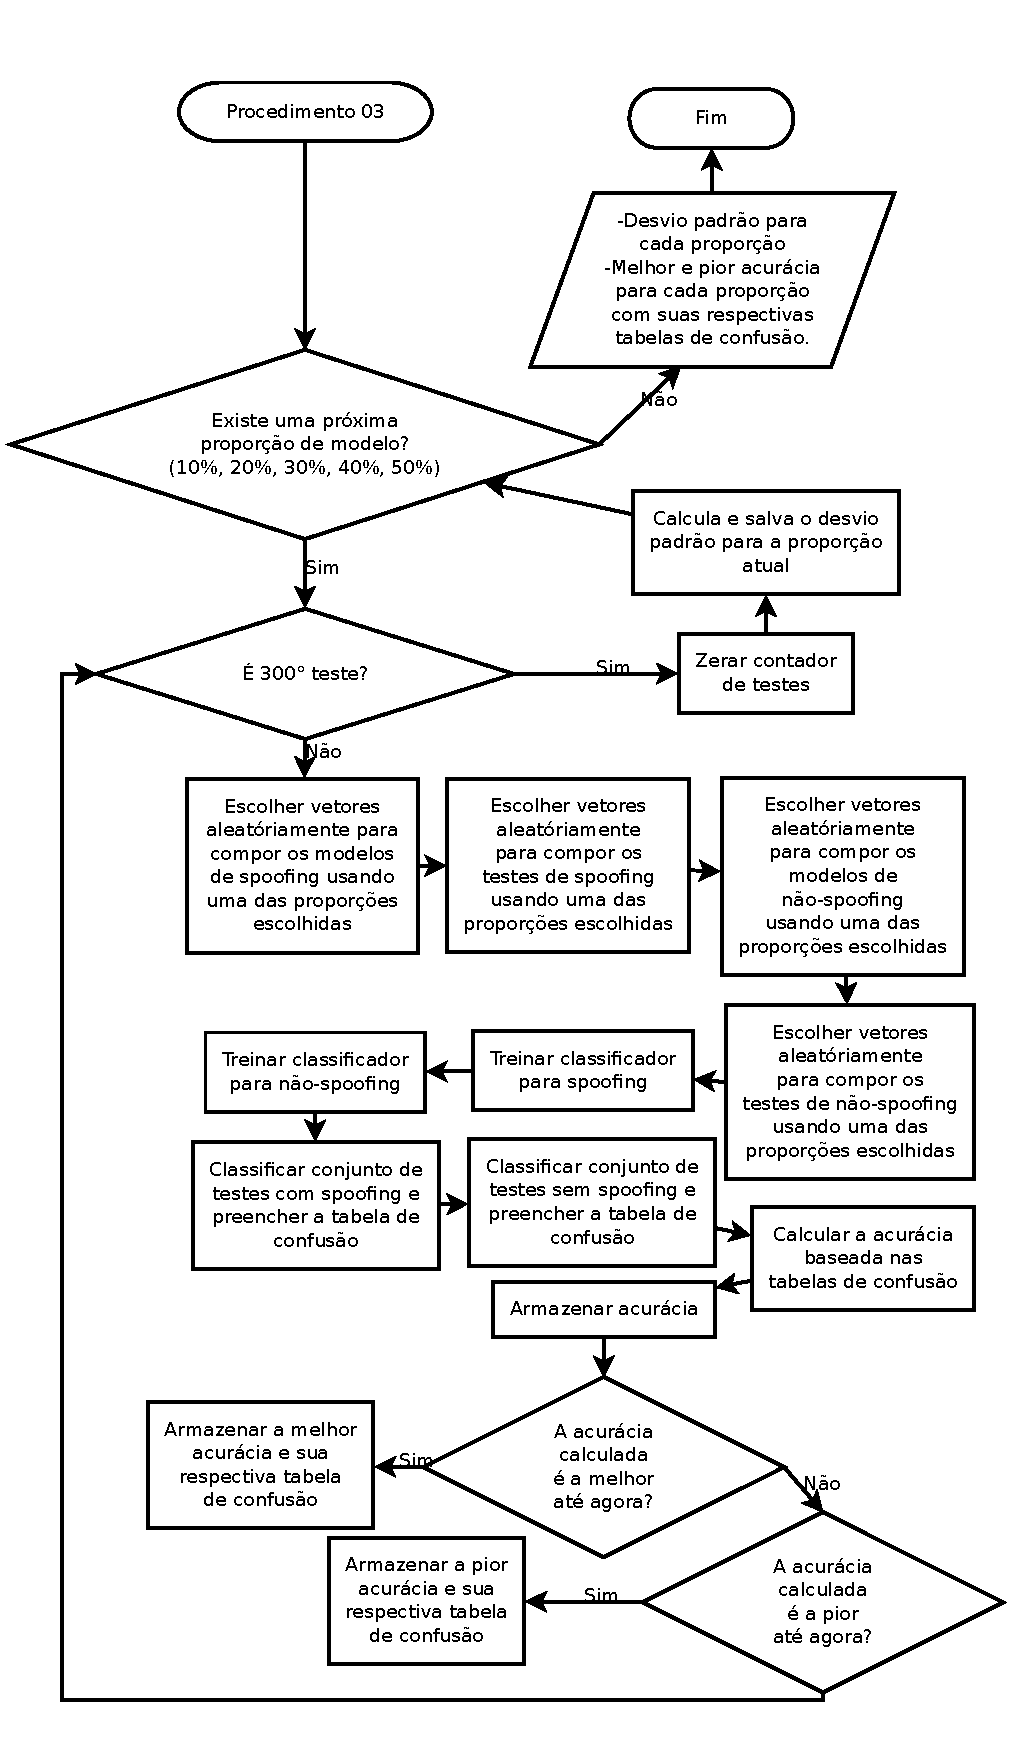
\includegraphics[width=0.9\linewidth]{images/AlgoProcedure03}
			\label{fig:experiment03Algo}
			\\Fonte: Elaborado pelo autor, 2021.
		\end{figure}

        \par Os testes e resultados dos experimentos descritos neste Capítulo encontram-se no Capítulo seguinte.

	
	\chapter{Testes e Resultados} \label{chap:testsResults}
	\section{Experimento 01}
	\begin{figure}[h]
		\centering
		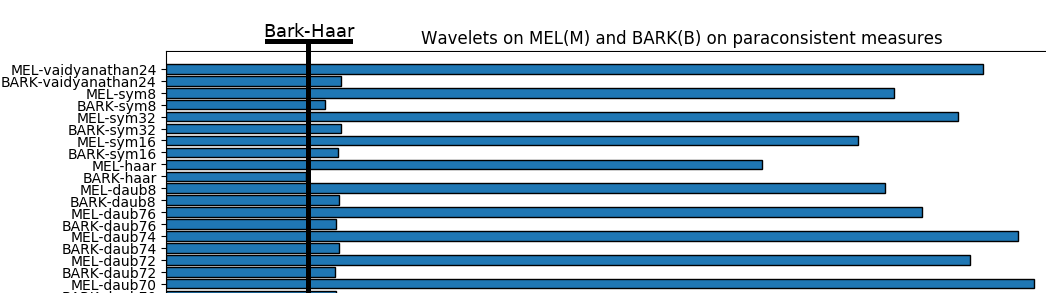
\includegraphics[width=\linewidth]{images/results/paraconsistentPlane/ParaconsistentParcial.png}
		\caption{Distância da combinação Wavelet\textit{X}BARK ou MEL do ponto (1,0)}
		\label{fig:ParaconsistentParcial}
	\end{figure}

	\begin{table}[h]
	\newcommand{\mc}[3]{\multicolumn{#1}{#2}{#3}}
	\definecolor{tcB}{rgb}{0.447059,0.74902,0.266667}
	\definecolor{tcA}{rgb}{0.65098,0.65098,0.65098}
	\definecolor{tcC}{rgb}{1,0.94902,0}
	\begin{center}
		\begin{tabular}{|c|c|c|c|}\hline
			% use packages: color,colortbl
			\rowcolor{tcA}
			Wavelet & G1 & G2 & Distancia do ponto (1,0)\\\hline
			\rowcolor{tcB}
			haar & 0.93615 & 4.68316e-310 & 0.0638503\\\hline
			\mc{1}{|>{\columncolor{tcC}}c|}{daub4} & \mc{1}{>{\columncolor{tcC}}c|}{0.928088} & \mc{1}{>{\columncolor{tcC}}c|}{4.68316e-310} & \mc{1}{>{\columncolor{tcC}}c|}{0.0719123}\\\hline
			\mc{1}{|>{\columncolor{tcC}}c|}{daub6} & \mc{1}{>{\columncolor{tcC}}c|}{0.927885} & \mc{1}{>{\columncolor{tcC}}c|}{4.68316e-310} & \mc{1}{>{\columncolor{tcC}}c|}{0.072115}\\\hline
			\mc{1}{|>{\columncolor{tcC}}c|}{coif6} & \mc{1}{>{\columncolor{tcC}}c|}{0.927823} & \mc{1}{>{\columncolor{tcC}}c|}{4.68316e-310} & \mc{1}{>{\columncolor{tcC}}c|}{0.072177}\\\hline
			\mc{1}{|>{\columncolor{tcC}}c|}{sym8} & \mc{1}{>{\columncolor{tcC}}c|}{0.92769} & \mc{1}{>{\columncolor{tcC}}c|}{4.68316e-310} & \mc{1}{>{\columncolor{tcC}}c|}{0.0723096}\\\hline
			\mc{1}{|>{\columncolor{tcC}}c|}{daub12} & \mc{1}{>{\columncolor{tcC}}c|}{0.926541} & \mc{1}{>{\columncolor{tcC}}c|}{4.68316e-310} & \mc{1}{>{\columncolor{tcC}}c|}{0.073459}\\\hline
		\end{tabular}
	\end{center}
	\caption{Wavelet\textit{X}BARK no plano paraconsistente}
	\label{tab:distParacomBest}
\end{table}

	\par Na figura \ref{fig:ParaconsistentParcial} quanto menor o valor, mais disjuntos tendem ser os vetores de características gerados para as duas classes testadas (\textit{spoofing }e não \textit{spoofing}). Como se pode constatar, das combinações testadas, a \textit{\textbf{Haar com BARK}} conseguiu o \textbf{melhor desempenho} na criação dos melhores vetores de características. A tabela \ref{tab:distParacomBest} mostra os 6 melhores resultados em distância do ponto (1,0)(verdade) no plano paraconsistente, a totalidade dos dados se encontram no apêndice deste documento nas tabelas \ref{tab:distParacomFrom10Bark_1} e \ref{tab:distParacomFrom10Bark_2} para todos os resultados com BARK e nas tabelas \ref{tab:distParacomFrom10Mel_1} e \ref{tab:distParacomFrom10Mel_2} para os com MEL. Na figura \ref{fig:paraconsistentfull} se pode ver o gráfico de barras para todas as combinações \textit{wavelets}X\textit{BARK/MEL}.
	
	\par A combinação \textbf{\textit{wavelet + BARK}} teve, consistentemente, um desempenho \textbf{melhor} do que as respectivas combinações \textbf{\textit{wavelet + MEL}}.
	
	\newpage
	\section{Experimento 02}
		\par Considerando que o experimento 1 teve como melhor resultado a combinação \textbf{Haar+BARK} o objetivo deste é constatar a máxima acurácia que se consegue atingir em um classificador baseado em distâncias Euclidianas e Manhattan. O dimensionamento do tamanho das amostras de referência que neste caso são os itens usados para o treinamento do classificador variou em 10\%, 20\%, 30\%, 40\% e finalmente 50\% do total das amostras. 300 foi a quantidade máxima de testes escolhida.
		\par Os resultados gerais são mostrados na tabela \ref{tab:experiment02ResultsEuclidian} para distância Euclidiana e na tabela \ref{tab:experiment02ResultsManhattan} para distância Manhattan. 
		
		\par Mais níveis de detalhes para a distância Euclidiana pode ser conseguido consultando-se as tabelas \ref{tab:classifier_Euclidian_10}, \ref{tab:classifier_Euclidian_20}, \ref{tab:classifier_Euclidian_30}, \ref{tab:classifier_Euclidian_40},  \ref{tab:classifier_Euclidian_50} e seus respectivos gráficos \ref{fig:classifiereuclidian10}, \ref{fig:classifiereuclidian20}, \ref{fig:classifiereuclidian30}, \ref{fig:classifiereuclidian40}, \ref{fig:classifiereuclidian50}.
		
		\par E para a distância Manhattan podem ser consultadas as tabelas 	\ref{tab:classifier_Manhattan_10}, \ref{tab:classifier_Manhattan_20}, \ref{tab:classifier_Manhattan_30}, \ref{tab:classifier_Manhattan_40}, \ref{tab:classifier_Manhattan_50} e seus respectivos gráficos 		 
		 \ref{fig:classifiermanhattan10}, \ref{fig:classifiermanhattan20}, 	 \ref{fig:classifiermanhattan30}, \ref{fig:classifiermanhattan40},  \ref{fig:classifiermanhattan50}.
			\begin{table}[h]
	\newcommand{\mc}[3]{\multicolumn{#1}{#2}{#3}}
	\definecolor{tcA}{rgb}{0.65098,0.65098,0.65098}
	\definecolor{tcB}{rgb}{0.447059,0.74902,0.266667}
	\begin{center}
		\begin{tabular}{|l|l|l|}\hline
			% use packages: color,colortbl
			\rowcolor{tcA}
			\textbf{Tamanho do modelo} & \textbf{Acurácia mínima} & \textbf{Acurácia máxima}\\\hline
			\rowcolor{tcB}
			\mc{1}{|c|}{10\%} & \mc{1}{c|}{0,6666} & \mc{1}{c|}{0,8861}\\\hline
			\rowcolor{tcB}
			\mc{1}{|c|}{20\%} & \mc{1}{c|}{0,7439} & \mc{1}{c|}{0,8902}\\\hline
			\rowcolor{tcB}
			\mc{1}{|c|}{30\%} & \mc{1}{c|}{0,7665} & \mc{1}{c|}{0,8919}\\\hline
			\rowcolor{tcB}
			\mc{1}{|c|}{40\%} & \mc{1}{c|}{0,7784} & \mc{1}{c|}{0,9024}\\\hline
			\rowcolor{tcB}
			\mc{1}{|c|}{50\%} & \mc{1}{c|}{0,7804} & \mc{1}{c|}{0,9097}\\\hline
		\end{tabular}
	\end{center}
	\caption{Resultados do experimento 02}
	\label{tab:experiment02Results}
\end{table}
			
			\newpage
			\begin{figure}[h]
				\centering
				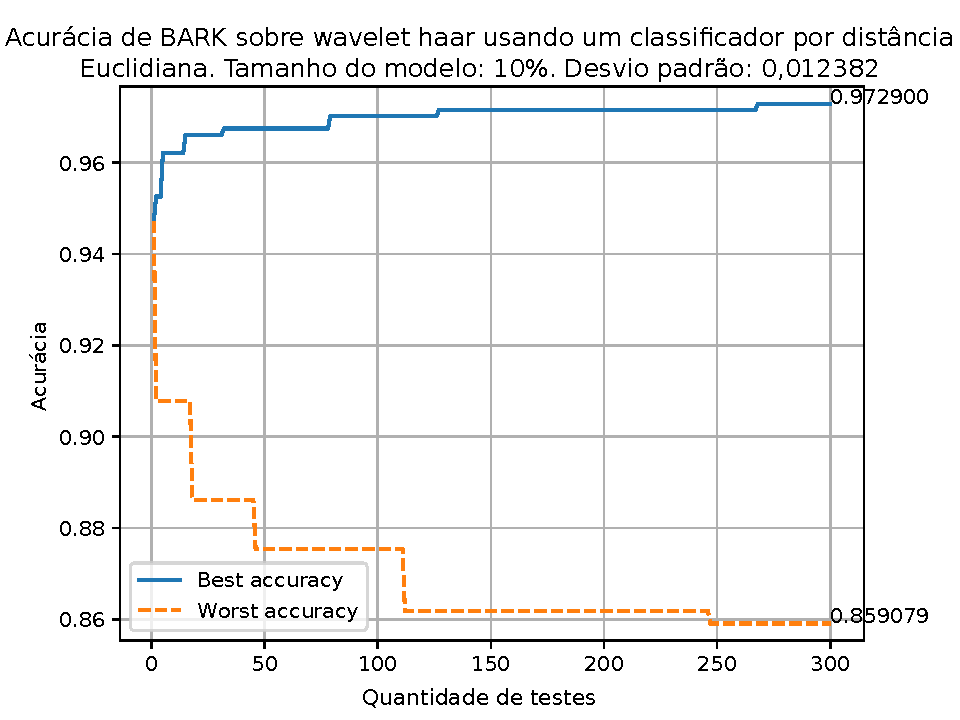
\includegraphics{images/results/confusionMatrices/classifier_Euclidian_10}
				\caption{Acurácia \textit{X} quantidade de testes - Distância Euclidiana, modelo a 10\%}
				\label{fig:classifiereuclidian10}
			\end{figure}
			\begin{table}[H] 					\newcommand{\mc}[3]{\multicolumn{#1}{#2}{#3}} 					\definecolor{tcB}{rgb}{0.447059,0.74902,0.266667} 					\definecolor{tcC}{rgb}{0,0,0} 					\definecolor{tcD}{rgb}{0,0.5,1} 					\definecolor{tcA}{rgb}{0.65098,0.65098,0.65098} 					\begin{center} 						\subfloat[Melhor matriz de confusão]{ 							\begin{tabular}{ccc} 								\mc{1}{l}{} & \mc{1}{>{\columncolor{tcA}}c}{\textbf{genuíno}} & \mc{1}{>{\columncolor{tcA}}c}{\textbf{falseado}}\\ 								\mc{1}{>{\columncolor{tcA}}r}{\textbf{genuíno}} & \mc{1}{>{\columncolor{tcB}}c}{\textcolor{tcC}{363}} & \mc{1}{>{\columncolor{tcD}}c}{\textcolor{tcC}{14}}\\ 								\mc{1}{>{\columncolor{tcA}}r}{\textbf{falseado}} & \mc{1}{>{\columncolor{tcD}}c}{\textcolor{tcC}{6}} & \mc{1}{>{\columncolor{tcB}}c}{\textcolor{tcC}{355}} 							\end{tabular} 							\label{tab:classifier_Euclidian_10_best} 						} 						\qquad 						\subfloat[Pior matriz de confusão]{ 							\begin{tabular}{ccc} 								\mc{1}{l}{} & \mc{1}{>{\columncolor{tcA}}c}{\textbf{genuíno}} & \mc{1}{>{\columncolor{tcA}}c}{\textbf{falseado}}\\ 								\mc{1}{>{\columncolor{tcA}}r}{\textbf{genuíno}} & \mc{1}{>{\columncolor{tcB}}c}{\textcolor{tcC}{275}} & \mc{1}{>{\columncolor{tcD}}c}{\textcolor{tcC}{10}}\\ 								\mc{1}{>{\columncolor{tcA}}r}{\textbf{falseado}} & \mc{1}{>{\columncolor{tcD}}c}{\textcolor{tcC}{94}} & \mc{1}{>{\columncolor{tcB}}c}{\textcolor{tcC}{359}} 							\end{tabular} 							\label{tab:classifier_Euclidian_10_worse} 						} 					\end{center} 					\caption{Matrizes de confusão para distância Euclidiana com modelo a 10\%} 				\end{table}
			\newpage
			\begin{figure}[h]
				\centering
				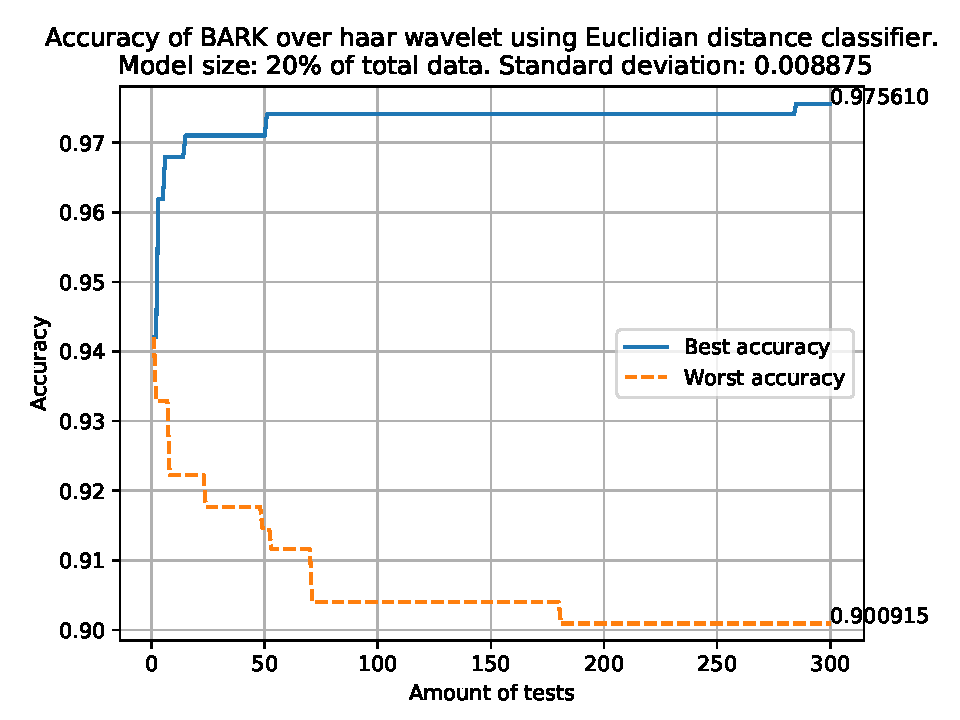
\includegraphics{images/results/confusionMatrices/classifier_Euclidian_20}
				\caption{Acurácia \textit{X} quantidade de testes - Distância Euclidiana, modelo a 20\%}
				\label{fig:classifiereuclidian20}
			\end{figure}
			\begin{table}[h]
\newcommand{\mc}[3]{\multicolumn{#1}{#2}{#3}}
\definecolor{tcB}{rgb}{0.447059,0.74902,0.266667}
\definecolor{tcC}{rgb}{0,0,0}
\definecolor{tcD}{rgb}{0,0.4,0.701961}
\definecolor{tcA}{rgb}{0.65098,0.65098,0.65098}
\begin{center}
	\begin{tabular}{ccc}
		% use packages: color,colortbl
		\mc{1}{l}{} & \mc{1}{>{\columncolor{tcA}}c}{\textbf{genuíno}} & \mc{1}{>{\columncolor{tcA}}c}{\textbf{regravado}}\\

		\mc{1}{>{\columncolor{tcA}}r}{\textbf{genuíno}} & \mc{1}{>{\columncolor{tcB}}c}{\textcolor{tcC}{308}} & \mc{1}{>{\columncolor{tcD}}c}{\textcolor{tcC}{50}}\\

		\mc{1}{>{\columncolor{tcA}}r}{\textbf{regravado}} & \mc{1}{>{\columncolor{tcD}}c}{\textcolor{tcC}{20}} & \mc{1}{>{\columncolor{tcB}}c}{\textcolor{tcC}{278}}
	\end{tabular}
	\caption{Melhor matriz de confusão para o classificador por distâncias Euclidianas com o uso de 20\% da base para modelagem}
	\label{tab:classifier_Euclidian_20_best}
\end{center}
\end{table}

\begin{table}[h]
	\newcommand{\mc}[3]{\multicolumn{#1}{#2}{#3}}
	\definecolor{tcB}{rgb}{0.447059,0.74902,0.266667}
	\definecolor{tcC}{rgb}{0,0,0}
	\definecolor{tcD}{rgb}{0,0.4,0.701961}
	\definecolor{tcA}{rgb}{0.65098,0.65098,0.65098}
	\begin{center}
		\begin{tabular}{ccc}
			% use packages: color,colortbl
			\mc{1}{l}{} & \mc{1}{>{\columncolor{tcA}}c}{\textbf{genuíno}} & \mc{1}{>{\columncolor{tcA}}c}{\textbf{regravado}}\\
			
			\mc{1}{>{\columncolor{tcA}}r}{\textbf{genuíno}} & \mc{1}{>{\columncolor{tcB}}c}{\textcolor{tcC}{295}} & \mc{1}{>{\columncolor{tcD}}c}{\textcolor{tcC}{137}}\\
			
			\mc{1}{>{\columncolor{tcA}}r}{\textbf{regravado}} & \mc{1}{>{\columncolor{tcD}}c}{\textcolor{tcC}{33}} & \mc{1}{>{\columncolor{tcB}}c}{\textcolor{tcC}{191}}
		\end{tabular}
		\caption{Pior matriz de confusão para o classificador por distâncias Euclidianas com o uso de 20\% da base para modelagem}
		\label{tab:classifier_Euclidian_20_worse}
	\end{center}
\end{table}

	
			\newpage
			\begin{figure}[h]
				\centering
				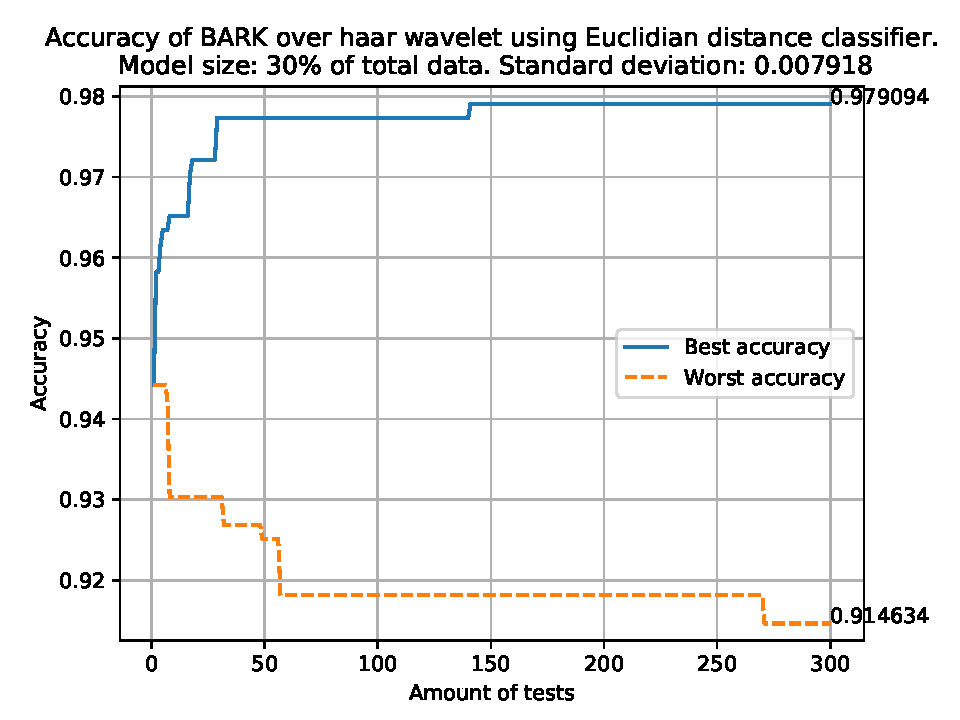
\includegraphics{images/results/confusionMatrices/classifier_Euclidian_30}
				\caption{Acurácia \textit{X} quantidade de testes - Distância Euclidiana, modelo a 30\%}
				\label{fig:classifiereuclidian30}
			\end{figure}
			\begin{table}[H] 					\newcommand{\mc}[3]{\multicolumn{#1}{#2}{#3}} 					\definecolor{tcB}{rgb}{0.447059,0.74902,0.266667} 					\definecolor{tcC}{rgb}{0,0,0} 					\definecolor{tcD}{rgb}{0,0.5,1} 					\definecolor{tcA}{rgb}{0.65098,0.65098,0.65098} 					\begin{center} 		\caption{Matrizes de confusão para distância Euclidiana com modelo a 30\%}				\subfloat[Melhor matriz de confusão]{ 							\begin{tabular}{ccc} 								\mc{1}{l}{} & \mc{1}{>{\columncolor{tcA}}c}{\textbf{genuíno}} & \mc{1}{>{\columncolor{tcA}}c}{\textbf{falseado}}\\ 								\mc{1}{>{\columncolor{tcA}}r}{\textbf{genuíno}} & \mc{1}{>{\columncolor{tcB}}c}{\textcolor{tcC}{283}} & \mc{1}{>{\columncolor{tcD}}c}{\textcolor{tcC}{8}}\\ 								\mc{1}{>{\columncolor{tcA}}r}{\textbf{falseado}} & \mc{1}{>{\columncolor{tcD}}c}{\textcolor{tcC}{4}} & \mc{1}{>{\columncolor{tcB}}c}{\textcolor{tcC}{279}} 							\end{tabular} 							\label{tab:classifier_Euclidian_30_best} 						} 						\qquad 						\subfloat[Pior matriz de confusão]{ 							\begin{tabular}{ccc} 								\mc{1}{l}{} & \mc{1}{>{\columncolor{tcA}}c}{\textbf{genuíno}} & \mc{1}{>{\columncolor{tcA}}c}{\textbf{falseado}}\\ 								\mc{1}{>{\columncolor{tcA}}r}{\textbf{genuíno}} & \mc{1}{>{\columncolor{tcB}}c}{\textcolor{tcC}{258}} & \mc{1}{>{\columncolor{tcD}}c}{\textcolor{tcC}{20}}\\ 								\mc{1}{>{\columncolor{tcA}}r}{\textbf{falseado}} & \mc{1}{>{\columncolor{tcD}}c}{\textcolor{tcC}{29}} & \mc{1}{>{\columncolor{tcB}}c}{\textcolor{tcC}{267}} 							\end{tabular} 							\label{tab:classifier_Euclidian_30_worse} 						} 					\\Fonte: Elaborado pelo autor, 2021.		\end{center} 					 				\end{table}
	
			\newpage	
			\begin{figure}[h]
				\centering
				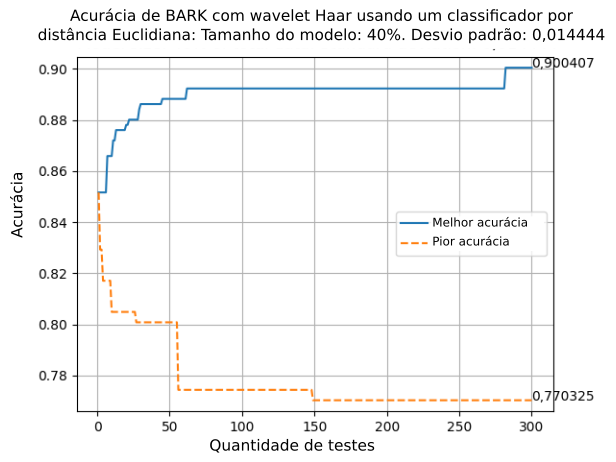
\includegraphics{images/results/confusionMatrices/classifier_Euclidian_40}
				\caption{Acurácia \textit{X} quantidade de testes - Distância Euclidiana, modelo a 40\%}
				\label{fig:classifiereuclidian40}
			\end{figure}
			\begin{table}[h]
\newcommand{\mc}[3]{\multicolumn{#1}{#2}{#3}}
\definecolor{tcB}{rgb}{0.447059,0.74902,0.266667}
\definecolor{tcC}{rgb}{0,0,0}
\definecolor{tcD}{rgb}{0,0.4,0.701961}
\definecolor{tcA}{rgb}{0.65098,0.65098,0.65098}
\begin{center}
	\begin{tabular}{ccc}
		% use packages: color,colortbl
		\mc{1}{l}{} & \mc{1}{>{\columncolor{tcA}}c}{\textbf{Verdadeiro}} & \mc{1}{>{\columncolor{tcA}}c}{\textbf{Falso}}\\

		\mc{1}{>{\columncolor{tcA}}r}{\textbf{Verdadeiro}} & \mc{1}{>{\columncolor{tcB}}c}{\textcolor{tcC}{233}} & \mc{1}{>{\columncolor{tcD}}c}{\textcolor{tcC}{35}}\\

		\mc{1}{>{\columncolor{tcA}}r}{\textbf{Falso}} & \mc{1}{>{\columncolor{tcD}}c}{\textcolor{tcC}{13}} & \mc{1}{>{\columncolor{tcB}}c}{\textcolor{tcC}{211}}
	\end{tabular}
	\caption{Tabela de confusão para classificador Euclidiano 40\%}
	\label{tab:classifier_Euclidian_40}
\end{center}
\end{table}

		
			\newpage
			\begin{figure}[h]
				\centering
				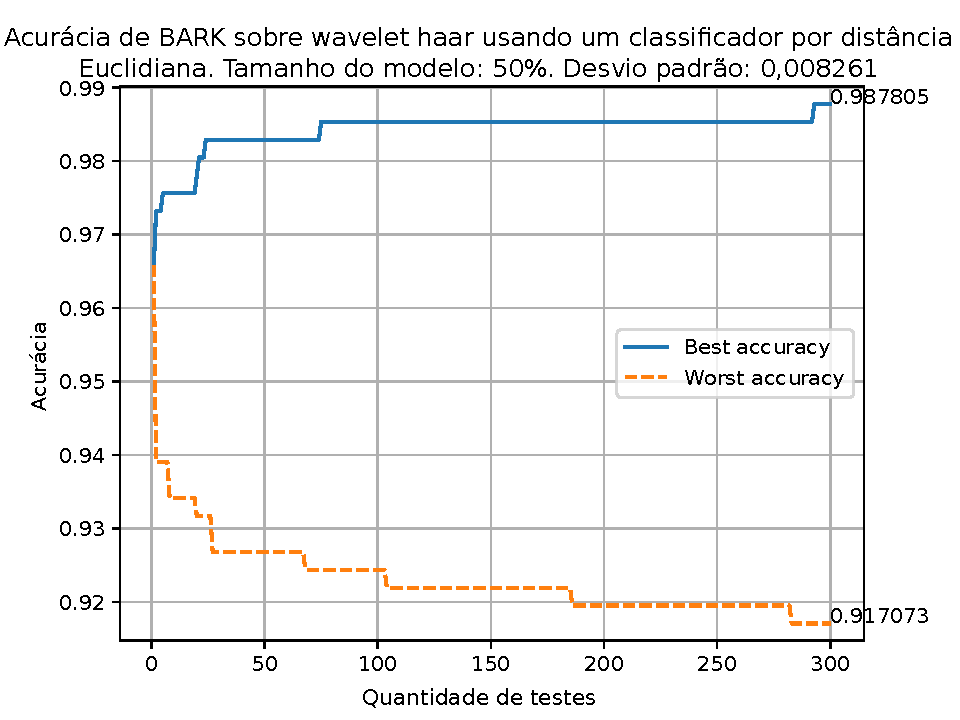
\includegraphics{images/results/confusionMatrices/classifier_Euclidian_50}
				\caption{Acurácia \textit{X} quantidade de testes - Distância Euclidiana, modelo a 50\%}
				\label{fig:classifiereuclidian50}
			\end{figure}
			\begin{table}[H]
	\newcommand{\mc}[3]{\multicolumn{#1}{#2}{#3}}
	\definecolor{tcB}{rgb}{0.447059,0.74902,0.266667}
	\definecolor{tcC}{rgb}{0,0,0}
	\definecolor{tcD}{rgb}{0,0.5,1}
	\definecolor{tcA}{rgb}{0.65098,0.65098,0.65098}
	\begin{center}
		\subfloat[Best matrix]{
			\begin{tabular}{ccc}
				% use packages: color,colortbl
				\mc{1}{l}{} & \mc{1}{>{\columncolor{tcA}}c}{\textbf{genuine}} & \mc{1}{>{\columncolor{tcA}}c}{\textbf{spoofed}}\\
				
				\mc{1}{>{\columncolor{tcA}}r}{\textbf{genuine}} & \mc{1}{>{\columncolor{tcB}}c}{\textcolor{tcC}{195}} & \mc{1}{>{\columncolor{tcD}}c}{\textcolor{tcC}{29}}\\
				
				\mc{1}{>{\columncolor{tcA}}r}{\textbf{spoofed}} & \mc{1}{>{\columncolor{tcD}}c}{\textcolor{tcC}{10}} & \mc{1}{>{\columncolor{tcB}}c}{\textcolor{tcC}{176}}
			\end{tabular}
			\label{tab:classifier_Euclidian_50_best}
		}
		\qquad
		\subfloat[Worst matrix]{
			\begin{tabular}{ccc}
				% use packages: color,colortbl
				\mc{1}{l}{} & \mc{1}{>{\columncolor{tcA}}c}{\textbf{genuine}} & \mc{1}{>{\columncolor{tcA}}c}{\textbf{spoofed}}\\
				
				\mc{1}{>{\columncolor{tcA}}r}{\textbf{genuine}} & \mc{1}{>{\columncolor{tcB}}c}{\textcolor{tcC}{193}} & \mc{1}{>{\columncolor{tcD}}c}{\textcolor{tcC}{79}}\\
				
				\mc{1}{>{\columncolor{tcA}}r}{\textbf{spoofed}} & \mc{1}{>{\columncolor{tcD}}c}{\textcolor{tcC}{12}} & \mc{1}{>{\columncolor{tcB}}c}{\textcolor{tcC}{126}}
			\end{tabular}
			\label{tab:classifier_Euclidian_50_worse}
		}
	\end{center}
	\caption{Confusion matrices for Euclidian distance classifier at 50\% model}
\end{table}
		
			\newpage
			\begin{figure}[h]
				\centering
				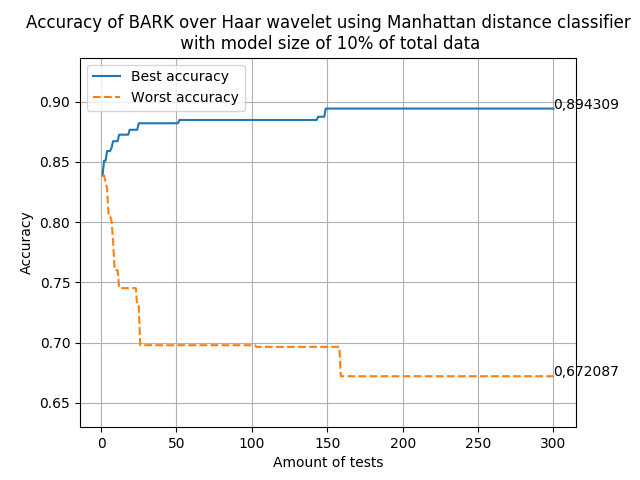
\includegraphics{images/results/confusionMatrices/classifier_Manhattan_10.png}
				\caption{Acurácia \textit{X} quantidade de testes - Distância Manhattan, modelo a 10\%}
				\label{fig:classifiermanhattan10}
			\end{figure}
			\begin{table}[h] 					\newcommand{\mc}[3]{\multicolumn{#1}{#2}{#3}} 					\definecolor{tcB}{rgb}{0.447059,0.74902,0.266667} 					\definecolor{tcC}{rgb}{0,0,0} 					\definecolor{tcD}{rgb}{0,0.5,1} 					\definecolor{tcA}{rgb}{0.65098,0.65098,0.65098} 					\begin{center} 						\subfloat[Melhor matriz de confusão]{ 							\begin{tabular}{ccc} 								\mc{1}{l}{} & \mc{1}{>{\columncolor{tcA}}c}{\textbf{genuíno}} & \mc{1}{>{\columncolor{tcA}}c}{\textbf{falsificado}}\\ 								\mc{1}{>{\columncolor{tcA}}r}{\textbf{genuíno}} & \mc{1}{>{\columncolor{tcB}}c}{\textcolor{tcC}{365}} & \mc{1}{>{\columncolor{tcD}}c}{\textcolor{tcC}{14}}\\ 								\mc{1}{>{\columncolor{tcA}}r}{\textbf{falsificado}} & \mc{1}{>{\columncolor{tcD}}c}{\textcolor{tcC}{4}} & \mc{1}{>{\columncolor{tcB}}c}{\textcolor{tcC}{355}} 							\end{tabular} 							\label{tab:classifier_Manhattan_10_best} 						} 						\qquad 						\subfloat[Pior matriz de confusão]{ 							\begin{tabular}{ccc} 								\mc{1}{l}{} & \mc{1}{>{\columncolor{tcA}}c}{\textbf{genuíno}} & \mc{1}{>{\columncolor{tcA}}c}{\textbf{falsificado}}\\ 								\mc{1}{>{\columncolor{tcA}}r}{\textbf{genuíno}} & \mc{1}{>{\columncolor{tcB}}c}{\textcolor{tcC}{289}} & \mc{1}{>{\columncolor{tcD}}c}{\textcolor{tcC}{11}}\\ 								\mc{1}{>{\columncolor{tcA}}r}{\textbf{falsificado}} & \mc{1}{>{\columncolor{tcD}}c}{\textcolor{tcC}{80}} & \mc{1}{>{\columncolor{tcB}}c}{\textcolor{tcC}{358}} 							\end{tabular} 							\label{tab:classifier_Manhattan_10_worse} 						} 					\end{center} 					\caption{Matrizes de confusão para distância Manhattan com modelo a 10\%} 				\end{table}
		
			\newpage
			\begin{figure}[h]
				\centering
				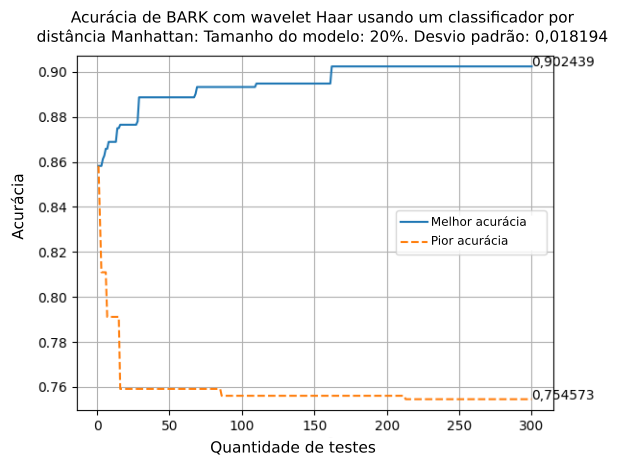
\includegraphics{images/results/confusionMatrices/classifier_Manhattan_20.png}
				\caption{Acurácia \textit{X} quantidade de testes - Distância Manhattan, modelo a 20\%}
				\label{fig:classifiermanhattan20}
			\end{figure}
			\begin{table}[h]
	\newcommand{\mc}[3]{\multicolumn{#1}{#2}{#3}}
	\definecolor{tcB}{rgb}{0.447059,0.74902,0.266667}
	\definecolor{tcC}{rgb}{0,0,0}
	\definecolor{tcD}{rgb}{0,0.5,1}
	\definecolor{tcA}{rgb}{0.65098,0.65098,0.65098}
	\begin{center}
		\subfloat[Melhor matriz]{
			\begin{tabular}{ccc}
				% use packages: color,colortbl
				\mc{1}{l}{} & \mc{1}{>{\columncolor{tcA}}c}{\textbf{Verdadeiro}} & \mc{1}{>{\columncolor{tcA}}c}{\textbf{Falso}}\\
				
				\mc{1}{>{\columncolor{tcA}}r}{\textbf{Verdadeiro}} & \mc{1}{>{\columncolor{tcB}}c}{\textcolor{tcC}{308}} & \mc{1}{>{\columncolor{tcD}}c}{\textcolor{tcC}{44}}\\
				
				\mc{1}{>{\columncolor{tcA}}r}{\textbf{Falso}} & \mc{1}{>{\columncolor{tcD}}c}{\textcolor{tcC}{20}} & \mc{1}{>{\columncolor{tcB}}c}{\textcolor{tcC}{284}}
			\end{tabular}
			\label{tab:classifier_Manhattan_20_best}
		}
		\qquad
		\subfloat[Pior matriz]{
			\begin{tabular}{ccc}
				% use packages: color,colortbl
				\mc{1}{l}{} & \mc{1}{>{\columncolor{tcA}}c}{\textbf{Verdadeiro}} & \mc{1}{>{\columncolor{tcA}}c}{\textbf{Falso}}\\
				
				\mc{1}{>{\columncolor{tcA}}r}{\textbf{Verdadeiro}} & \mc{1}{>{\columncolor{tcB}}c}{\textcolor{tcC}{316}} & \mc{1}{>{\columncolor{tcD}}c}{\textcolor{tcC}{149}}\\
				
				\mc{1}{>{\columncolor{tcA}}r}{\textbf{Falso}} & \mc{1}{>{\columncolor{tcD}}c}{\textcolor{tcC}{12}} & \mc{1}{>{\columncolor{tcB}}c}{\textcolor{tcC}{179}}
			\end{tabular}
			\label{tab:classifier_Manhattan_20_worst}
		}
	\end{center}
	\caption{Matrizes de confusão para o classificador por distâncias Manhattan com o uso de 20\% da base para modelagem}
\end{table}

	
			\newpage
			\begin{figure}[h]
				\centering
				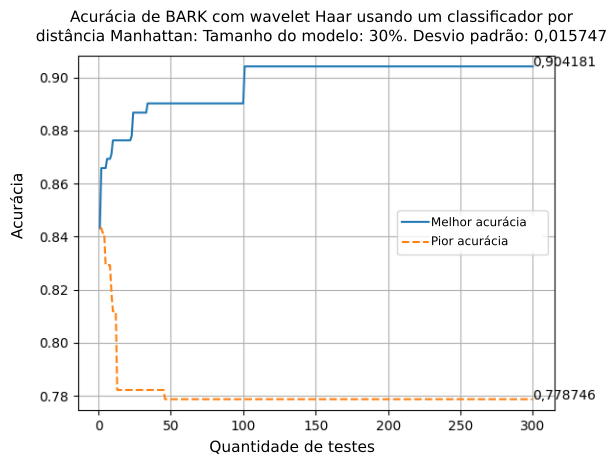
\includegraphics{images/results/confusionMatrices/classifier_Manhattan_30.png}
				\caption{Acurácia \textit{X} quantidade de testes - Distância Manhattan, modelo a 30\%}
				\label{fig:classifiermanhattan30}
			\end{figure}
			\begin{table}[h] 					\newcommand{\mc}[3]{\multicolumn{#1}{#2}{#3}} 					\definecolor{tcB}{rgb}{0.447059,0.74902,0.266667} 					\definecolor{tcC}{rgb}{0,0,0} 					\definecolor{tcD}{rgb}{0,0.5,1} 					\definecolor{tcA}{rgb}{0.65098,0.65098,0.65098} 					\begin{center} 						\subfloat[Melhor matriz de confusão]{ 							\begin{tabular}{ccc} 								\mc{1}{l}{} & \mc{1}{>{\columncolor{tcA}}c}{\textbf{genuíno}} & \mc{1}{>{\columncolor{tcA}}c}{\textbf{falsificado}}\\ 								\mc{1}{>{\columncolor{tcA}}r}{\textbf{genuíno}} & \mc{1}{>{\columncolor{tcB}}c}{\textcolor{tcC}{281}} & \mc{1}{>{\columncolor{tcD}}c}{\textcolor{tcC}{2}}\\ 								\mc{1}{>{\columncolor{tcA}}r}{\textbf{falsificado}} & \mc{1}{>{\columncolor{tcD}}c}{\textcolor{tcC}{6}} & \mc{1}{>{\columncolor{tcB}}c}{\textcolor{tcC}{285}} 							\end{tabular} 							\label{tab:classifier_Manhattan_30_best} 						} 						\qquad 						\subfloat[Pior matriz de confusão]{ 							\begin{tabular}{ccc} 								\mc{1}{l}{} & \mc{1}{>{\columncolor{tcA}}c}{\textbf{genuíno}} & \mc{1}{>{\columncolor{tcA}}c}{\textbf{falsificado}}\\ 								\mc{1}{>{\columncolor{tcA}}r}{\textbf{genuíno}} & \mc{1}{>{\columncolor{tcB}}c}{\textcolor{tcC}{256}} & \mc{1}{>{\columncolor{tcD}}c}{\textcolor{tcC}{19}}\\ 								\mc{1}{>{\columncolor{tcA}}r}{\textbf{falsificado}} & \mc{1}{>{\columncolor{tcD}}c}{\textcolor{tcC}{31}} & \mc{1}{>{\columncolor{tcB}}c}{\textcolor{tcC}{268}} 							\end{tabular} 							\label{tab:classifier_Manhattan_30_worse} 						} 					\end{center} 					\caption{Matrizes de confusão para distância Manhattan com modelo a 30\%} 				\end{table}
			
			\newpage
			\begin{figure}[h]
				\centering
				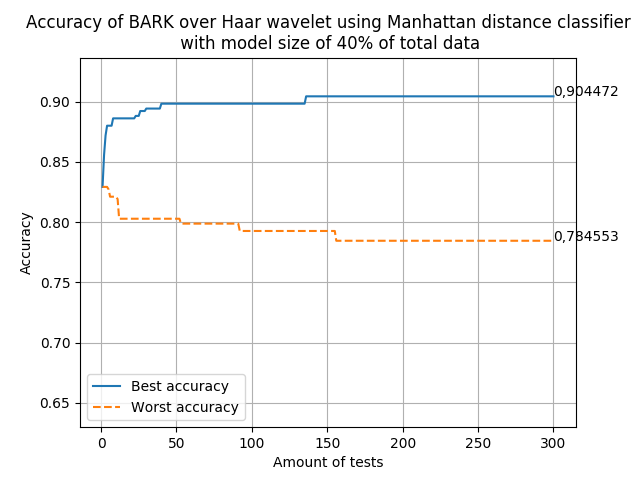
\includegraphics{images/results/confusionMatrices/classifier_Manhattan_40.png}
				\caption{Acurácia \textit{X} quantidade de testes - Distância Manhattan, modelo a 40\%}
				\label{fig:classifiermanhattan40}
			\end{figure}
			\begin{table}[h] 					\newcommand{\mc}[3]{\multicolumn{#1}{#2}{#3}} 					\definecolor{tcB}{rgb}{0.447059,0.74902,0.266667} 					\definecolor{tcC}{rgb}{0,0,0} 					\definecolor{tcD}{rgb}{0,0.5,1} 					\definecolor{tcA}{rgb}{0.65098,0.65098,0.65098} 					\begin{center} 						\subfloat[Best confusion matrix]{ 							\begin{tabular}{ccc} 								\mc{1}{l}{} & \mc{1}{>{\columncolor{tcA}}c}{\textbf{genuine}} & \mc{1}{>{\columncolor{tcA}}c}{\textbf{spoofed}}\\ 								\mc{1}{>{\columncolor{tcA}}r}{\textbf{genuine}} & \mc{1}{>{\columncolor{tcB}}c}{\textcolor{tcC}{244}} & \mc{1}{>{\columncolor{tcD}}c}{\textcolor{tcC}{5}}\\ 								\mc{1}{>{\columncolor{tcA}}r}{\textbf{spoofed}} & \mc{1}{>{\columncolor{tcD}}c}{\textcolor{tcC}{2}} & \mc{1}{>{\columncolor{tcB}}c}{\textcolor{tcC}{241}} 							\end{tabular} 							\label{tab:classifier_Manhattan_40_best} 						} 						\qquad 						\subfloat[Worst confusion matrix]{ 							\begin{tabular}{ccc} 								\mc{1}{l}{} & \mc{1}{>{\columncolor{tcA}}c}{\textbf{genuine}} & \mc{1}{>{\columncolor{tcA}}c}{\textbf{spoofed}}\\ 								\mc{1}{>{\columncolor{tcA}}r}{\textbf{genuine}} & \mc{1}{>{\columncolor{tcB}}c}{\textcolor{tcC}{218}} & \mc{1}{>{\columncolor{tcD}}c}{\textcolor{tcC}{7}}\\ 								\mc{1}{>{\columncolor{tcA}}r}{\textbf{spoofed}} & \mc{1}{>{\columncolor{tcD}}c}{\textcolor{tcC}{28}} & \mc{1}{>{\columncolor{tcB}}c}{\textcolor{tcC}{239}} 							\end{tabular} 							\label{tab:classifier_Manhattan_40_worse} 						} 					\end{center} 					\caption{Confusion matrices for Manhattan distance classifier at 40\% model} 				\end{table}
			
			\newpage
			\begin{figure}[h]
				\centering
				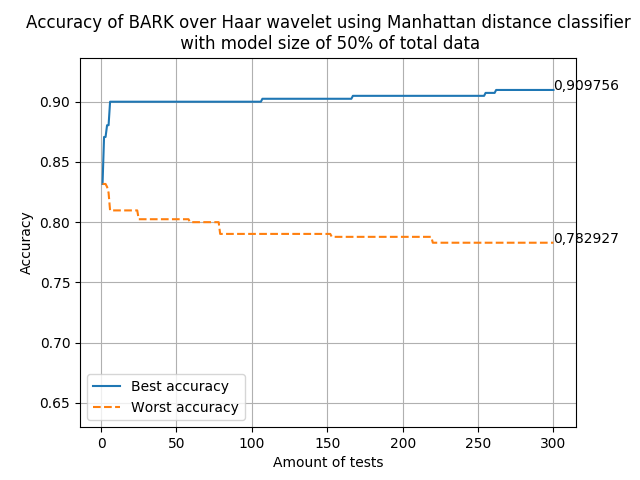
\includegraphics{images/results/confusionMatrices/classifier_Manhattan_50.png}
				\caption{Acurácia \textit{X} quantidade de testes - Distância Manhattan, modelo a 50\%}
				\label{fig:classifiermanhattan50}
			\end{figure}
			\begin{table}[h] 					\newcommand{\mc}[3]{\multicolumn{#1}{#2}{#3}} 					\definecolor{tcB}{rgb}{0.447059,0.74902,0.266667} 					\definecolor{tcC}{rgb}{0,0,0} 					\definecolor{tcD}{rgb}{0,0.5,1} 					\definecolor{tcA}{rgb}{0.65098,0.65098,0.65098} 					\begin{center} 						\subfloat[Best confusion matrix]{ 							\begin{tabular}{ccc} 								\mc{1}{l}{} & \mc{1}{>{\columncolor{tcA}}c}{\textbf{genuine}} & \mc{1}{>{\columncolor{tcA}}c}{\textbf{spoofed}}\\ 								\mc{1}{>{\columncolor{tcA}}r}{\textbf{genuine}} & \mc{1}{>{\columncolor{tcB}}c}{\textcolor{tcC}{172}} & \mc{1}{>{\columncolor{tcD}}c}{\textcolor{tcC}{30}}\\ 								\mc{1}{>{\columncolor{tcA}}r}{\textbf{spoofed}} & \mc{1}{>{\columncolor{tcD}}c}{\textcolor{tcC}{33}} & \mc{1}{>{\columncolor{tcB}}c}{\textcolor{tcC}{175}} 							\end{tabular} 							\label{tab:classifier_Manhattan_50_best} 						} 						\qquad 						\subfloat[Worst confusion matrix]{ 							\begin{tabular}{ccc} 								\mc{1}{l}{} & \mc{1}{>{\columncolor{tcA}}c}{\textbf{genuine}} & \mc{1}{>{\columncolor{tcA}}c}{\textbf{spoofed}}\\ 								\mc{1}{>{\columncolor{tcA}}r}{\textbf{genuine}} & \mc{1}{>{\columncolor{tcB}}c}{\textcolor{tcC}{142}} & \mc{1}{>{\columncolor{tcD}}c}{\textcolor{tcC}{58}}\\ 								\mc{1}{>{\columncolor{tcA}}r}{\textbf{spoofed}} & \mc{1}{>{\columncolor{tcD}}c}{\textcolor{tcC}{63}} & \mc{1}{>{\columncolor{tcB}}c}{\textcolor{tcC}{147}} 							\end{tabular} 							\label{tab:classifier_Manhattan_50_worse} 						} 					\end{center} 					\caption{Confusion matrices for Manhattan distance classifier at 50\% model} 				\end{table}
	
		\newpage
		\section{Experimento 03}
			\par Novamente, considerando que o experimento 1 teve como melhor resultado a combinação \textbf{Haar+BARK} o objetivo deste é constatar a máxima acurácia se consegue atingir em uma SVM. O dimensionamento do tamanho das amostras para o treinamento do classificador variou em 10\%, 20\%, 30\%, 40\% e finalmente 50\% do total das amostras. 300 foi a quantidade máxima de testes escolhida.
			
			\par Os resultados gerais são mostrados na tabela \ref{tab:experiment03Results}. 
			
			\par Mais níveis de detalhes podem ser consultados nas tabelas \ref{tab:classifier_SVM_10}, \ref{tab:classifier_Euclidian_20}, \ref{tab:classifier_SVM_30}, \ref{tab:classifier_Euclidian_40},  \ref{tab:classifier_SVM_50} e seus respectivos gráficos \ref{fig:classifiersvm10}, \ref{fig:classifiersvm20}, \ref{fig:classifiersvm30}, \ref{fig:classifiersvm40}, \ref{fig:classifiersvm50}.
	
			\begin{table}[H]
	\newcommand{\mc}[3]{\multicolumn{#1}{#2}{#3}}
	\definecolor{tcA}{rgb}{0.65098,0.65098,0.65098}
	\definecolor{tcB}{rgb}{0.447059,0.74902,0.266667}
	\begin{center}
		\caption{Resultados da abordagem com SVM}
		\begin{tabular}{|p{0.15\linewidth}|p{0.11\linewidth}|p{0.11\linewidth}|p{0.11\linewidth}|p{0.14\linewidth}|p{0.14\linewidth}|}\hline
			% use packages: color,colortbl
			\rowcolor{tcA}
			\centering\textbf{$M$} & \centering\textbf{Acurácia mínima} & \centering\textbf{Acurácia máxima} & \centering\textbf{Média das acurácias} & \centering\textbf{Desvio padrão da acurácia} & \begin{center}\textbf{EER}\end{center}\\\hline
			
			\rowcolor{tcB}
			% Loads data from tables/results/paraconsistentPlane/distParacomFrom10.csv
			\csvreader[
			late after line=\\\hline\rowcolor{tcB},%
			separator=comma,
			]{tables/results/experiment02ResultsSVM.csv}{1=\eme,2=\minAccu,3=\maxAccu,4=\meanAccu,5=\stdDev,6=\eer}{\centering\eme\% & \centering\StrSubstitute[0]{\minAccu}{.}{,} & \centering\StrSubstitute[0]{\maxAccu}{.}{,} & \centering\StrSubstitute[0]{\meanAccu}{.}{,} & \centering\StrSubstitute[0]{\stdDev}{.}{,} & \StrSubstitute[0]{\eer}{.}{,}}
			
		\end{tabular}
		\label{tab:experiment03Results}
		\\Fonte: Elaborado pelo autor, 2021.
	\end{center}
\end{table}
		
			\newpage
		\begin{figure}[h]
			\centering
			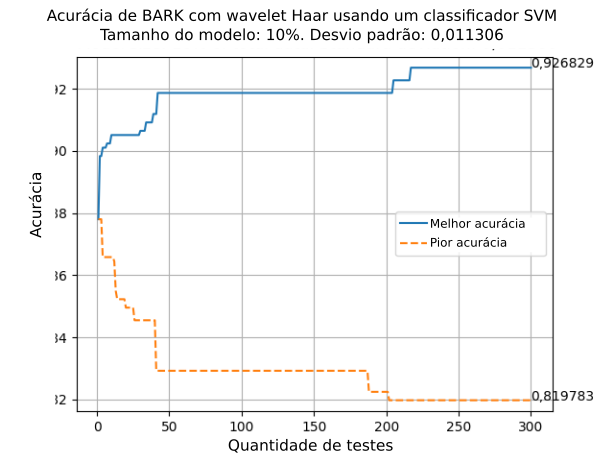
\includegraphics{images/results/confusionMatrices/classifier_SVM_10.png}
			\caption{Acurácia \textit{X} quantidade de testes - SVM, modelo a 10\%}
			\label{fig:classifiersvm10}
		\end{figure}
		\begin{table}[h]
\newcommand{\mc}[3]{\multicolumn{#1}{#2}{#3}}
\definecolor{tcB}{rgb}{0.447059,0.74902,0.266667}
\definecolor{tcC}{rgb}{0,0,0}
\definecolor{tcD}{rgb}{0,0.4,0.701961}
\definecolor{tcA}{rgb}{0.65098,0.65098,0.65098}
\begin{center}
	\begin{tabular}{ccc}
		% use packages: color,colortbl
		\mc{1}{l}{} & \mc{1}{>{\columncolor{tcA}}c}{\textbf{Verdadeiro}} & \mc{1}{>{\columncolor{tcA}}c}{\textbf{Falso}}\\

		\mc{1}{>{\columncolor{tcA}}r}{\textbf{Verdadeiro}} & \mc{1}{>{\columncolor{tcB}}c}{\textcolor{tcC}{339}} & \mc{1}{>{\columncolor{tcD}}c}{\textcolor{tcC}{24}}\\

		\mc{1}{>{\columncolor{tcA}}r}{\textbf{Falso}} & \mc{1}{>{\columncolor{tcD}}c}{\textcolor{tcC}{30}} & \mc{1}{>{\columncolor{tcB}}c}{\textcolor{tcC}{345}}
	\end{tabular}
	\caption{Melhor tabela de confusão para classificador SVM 10\%}
	\label{tab:classifier_SVM_10_best}
\end{center}
\end{table}

\begin{table}[h]
	\newcommand{\mc}[3]{\multicolumn{#1}{#2}{#3}}
	\definecolor{tcB}{rgb}{0.447059,0.74902,0.266667}
	\definecolor{tcC}{rgb}{0,0,0}
	\definecolor{tcD}{rgb}{0,0.4,0.701961}
	\definecolor{tcA}{rgb}{0.65098,0.65098,0.65098}
	\begin{center}
		\begin{tabular}{ccc}
			% use packages: color,colortbl
			\mc{1}{l}{} & \mc{1}{>{\columncolor{tcA}}c}{\textbf{Verdadeiro}} & \mc{1}{>{\columncolor{tcA}}c}{\textbf{Falso}}\\
			
			\mc{1}{>{\columncolor{tcA}}r}{\textbf{Verdadeiro}} & \mc{1}{>{\columncolor{tcB}}c}{\textcolor{tcC}{329}} & \mc{1}{>{\columncolor{tcD}}c}{\textcolor{tcC}{93}}\\
			
			\mc{1}{>{\columncolor{tcA}}r}{\textbf{Falso}} & \mc{1}{>{\columncolor{tcD}}c}{\textcolor{tcC}{40}} & \mc{1}{>{\columncolor{tcB}}c}{\textcolor{tcC}{276}}
		\end{tabular}
		\caption{Pior tabela de confusão para classificador SVM 10\%}
		\label{tab:classifier_SVM_10_worse}
	\end{center}
\end{table}

	
		\newpage
		\begin{figure}[h]
			\centering
			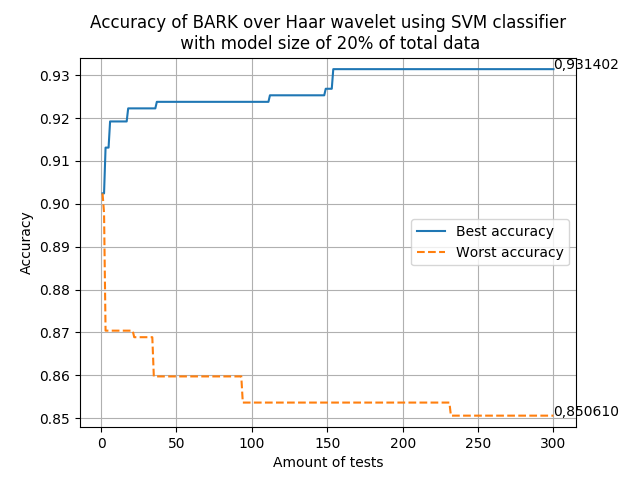
\includegraphics{images/results/confusionMatrices/classifier_SVM_20.png}
			\caption{Acurácia \textit{X} quantidade de testes - SVM, modelo a 20\%}
			\label{fig:classifiersvm20}
		\end{figure}
		\begin{table}[h] 					\newcommand{\mc}[3]{\multicolumn{#1}{#2}{#3}} 					\definecolor{tcB}{rgb}{0.447059,0.74902,0.266667} 					\definecolor{tcC}{rgb}{0,0,0} 					\definecolor{tcD}{rgb}{0,0.5,1} 					\definecolor{tcA}{rgb}{0.65098,0.65098,0.65098} 					\begin{center} 						\subfloat[Best confusion matrix]{ 							\begin{tabular}{ccc} 								\mc{1}{l}{} & \mc{1}{>{\columncolor{tcA}}c}{\textbf{genuine}} & \mc{1}{>{\columncolor{tcA}}c}{\textbf{spoofed}}\\ 								\mc{1}{>{\columncolor{tcA}}r}{\textbf{genuine}} & \mc{1}{>{\columncolor{tcB}}c}{\textcolor{tcC}{306}} & \mc{1}{>{\columncolor{tcD}}c}{\textcolor{tcC}{29}}\\ 								\mc{1}{>{\columncolor{tcA}}r}{\textbf{spoofed}} & \mc{1}{>{\columncolor{tcD}}c}{\textcolor{tcC}{22}} & \mc{1}{>{\columncolor{tcB}}c}{\textcolor{tcC}{299}} 							\end{tabular} 							\label{tab:classifier_Euclidian_10_best} 						} 						\qquad 						\subfloat[Worst confusion matrix]{ 							\begin{tabular}{ccc} 								\mc{1}{l}{} & \mc{1}{>{\columncolor{tcA}}c}{\textbf{genuine}} & \mc{1}{>{\columncolor{tcA}}c}{\textbf{spoofed}}\\ 								\mc{1}{>{\columncolor{tcA}}r}{\textbf{genuine}} & \mc{1}{>{\columncolor{tcB}}c}{\textcolor{tcC}{255}} & \mc{1}{>{\columncolor{tcD}}c}{\textcolor{tcC}{56}}\\ 								\mc{1}{>{\columncolor{tcA}}r}{\textbf{spoofed}} & \mc{1}{>{\columncolor{tcD}}c}{\textcolor{tcC}{73}} & \mc{1}{>{\columncolor{tcB}}c}{\textcolor{tcC}{272}} 							\end{tabular} 							\label{tab:classifier_Euclidian_10_worse} 						} 					\end{center} 					\caption{Confusion matrices for SVM classifier at 20\% model} 				\end{table}
		
		\newpage
		\begin{figure}[h]
			\centering
			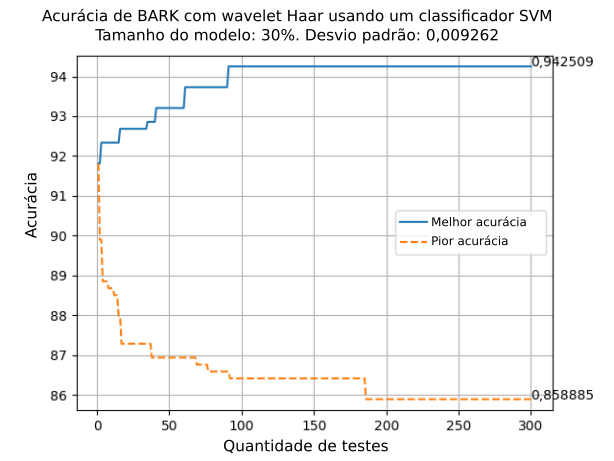
\includegraphics{images/results/confusionMatrices/classifier_SVM_30.png}
			\caption{Acurácia \textit{X} quantidade de testes - SVM, modelo a 30\%}
			\label{fig:classifiersvm30}
		\end{figure}
		\begin{table}[h] 					\newcommand{\mc}[3]{\multicolumn{#1}{#2}{#3}} 					\definecolor{tcB}{rgb}{0.447059,0.74902,0.266667} 					\definecolor{tcC}{rgb}{0,0,0} 					\definecolor{tcD}{rgb}{0,0.5,1} 					\definecolor{tcA}{rgb}{0.65098,0.65098,0.65098} 					\begin{center} 						\subfloat[Best confusion matrix]{ 							\begin{tabular}{ccc} 								\mc{1}{l}{} & \mc{1}{>{\columncolor{tcA}}c}{\textbf{genuine}} & \mc{1}{>{\columncolor{tcA}}c}{\textbf{spoofed}}\\ 								\mc{1}{>{\columncolor{tcA}}r}{\textbf{genuine}} & \mc{1}{>{\columncolor{tcB}}c}{\textcolor{tcC}{272}} & \mc{1}{>{\columncolor{tcD}}c}{\textcolor{tcC}{27}}\\ 								\mc{1}{>{\columncolor{tcA}}r}{\textbf{spoofed}} & \mc{1}{>{\columncolor{tcD}}c}{\textcolor{tcC}{15}} & \mc{1}{>{\columncolor{tcB}}c}{\textcolor{tcC}{260}} 							\end{tabular} 							\label{tab:classifier_Euclidian_10_best} 						} 						\qquad 						\subfloat[Worst confusion matrix]{ 							\begin{tabular}{ccc} 								\mc{1}{l}{} & \mc{1}{>{\columncolor{tcA}}c}{\textbf{genuine}} & \mc{1}{>{\columncolor{tcA}}c}{\textbf{spoofed}}\\ 								\mc{1}{>{\columncolor{tcA}}r}{\textbf{genuine}} & \mc{1}{>{\columncolor{tcB}}c}{\textcolor{tcC}{233}} & \mc{1}{>{\columncolor{tcD}}c}{\textcolor{tcC}{39}}\\ 								\mc{1}{>{\columncolor{tcA}}r}{\textbf{spoofed}} & \mc{1}{>{\columncolor{tcD}}c}{\textcolor{tcC}{54}} & \mc{1}{>{\columncolor{tcB}}c}{\textcolor{tcC}{248}} 							\end{tabular} 							\label{tab:classifier_Euclidian_10_worse} 						} 					\end{center} 					\caption{Confusion matrices for SVM classifier at 30\% model} 				\end{table}
	
		\newpage
		\begin{figure}[h]
			\centering
			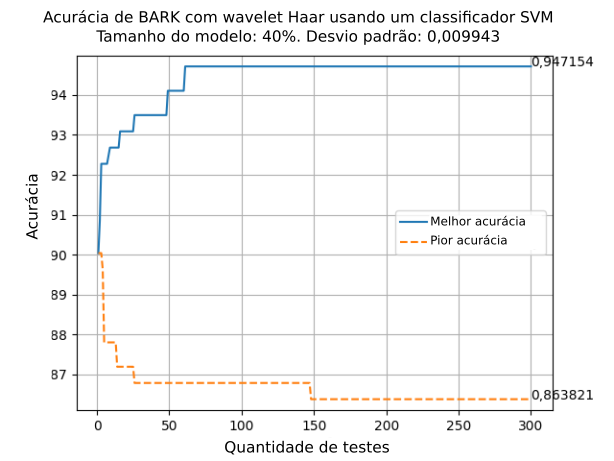
\includegraphics{images/results/confusionMatrices/classifier_SVM_40.png}
			\caption{Acurácia \textit{X} quantidade de testes - SVM, modelo a 40\%}
			\label{fig:classifiersvm40}
		\end{figure}
		\begin{table}[h]
\newcommand{\mc}[3]{\multicolumn{#1}{#2}{#3}}
\definecolor{tcB}{rgb}{0.447059,0.74902,0.266667}
\definecolor{tcC}{rgb}{0,0,0}
\definecolor{tcD}{rgb}{0,0.5,1}
\definecolor{tcA}{rgb}{0.65098,0.65098,0.65098}
\begin{center}
	\begin{tabular}{ccc}
		% use packages: color,colortbl
		\mc{1}{l}{} & \mc{1}{>{\columncolor{tcA}}c}{\textbf{Verdadeiro}} & \mc{1}{>{\columncolor{tcA}}c}{\textbf{Falso}}\\

		\mc{1}{>{\columncolor{tcA}}r}{\textbf{Verdadeiro}} & \mc{1}{>{\columncolor{tcB}}c}{\textcolor{tcC}{234}} & \mc{1}{>{\columncolor{tcD}}c}{\textcolor{tcC}{14}}\\

		\mc{1}{>{\columncolor{tcA}}r}{\textbf{Falso}} & \mc{1}{>{\columncolor{tcD}}c}{\textcolor{tcC}{12}} & \mc{1}{>{\columncolor{tcB}}c}{\textcolor{tcC}{232}}
	\end{tabular}
	\caption{Melhor tabela de confusão para classificador SVM 40\%}
	\label{tab:classifier_SVM_40_best}
\end{center}
\end{table}

\begin{table}[h]
	\newcommand{\mc}[3]{\multicolumn{#1}{#2}{#3}}
	\definecolor{tcB}{rgb}{0.447059,0.74902,0.266667}
	\definecolor{tcC}{rgb}{0,0,0}
	\definecolor{tcD}{rgb}{0,0.5,1}
	\definecolor{tcA}{rgb}{0.65098,0.65098,0.65098}
	\begin{center}
		\begin{tabular}{ccc}
			% use packages: color,colortbl
			\mc{1}{l}{} & \mc{1}{>{\columncolor{tcA}}c}{\textbf{Verdadeiro}} & \mc{1}{>{\columncolor{tcA}}c}{\textbf{Falso}}\\
			
			\mc{1}{>{\columncolor{tcA}}r}{\textbf{Verdadeiro}} & \mc{1}{>{\columncolor{tcB}}c}{\textcolor{tcC}{216}} & \mc{1}{>{\columncolor{tcD}}c}{\textcolor{tcC}{37}}\\
			
			\mc{1}{>{\columncolor{tcA}}r}{\textbf{Falso}} & \mc{1}{>{\columncolor{tcD}}c}{\textcolor{tcC}{30}} & \mc{1}{>{\columncolor{tcB}}c}{\textcolor{tcC}{209}}
		\end{tabular}
		\caption{Pior tabela de confusão para classificador SVM 40\%}
		\label{tab:classifier_SVM_40_worse}
	\end{center}
\end{table}

	
		\newpage
		\begin{figure}[h]
			\centering
			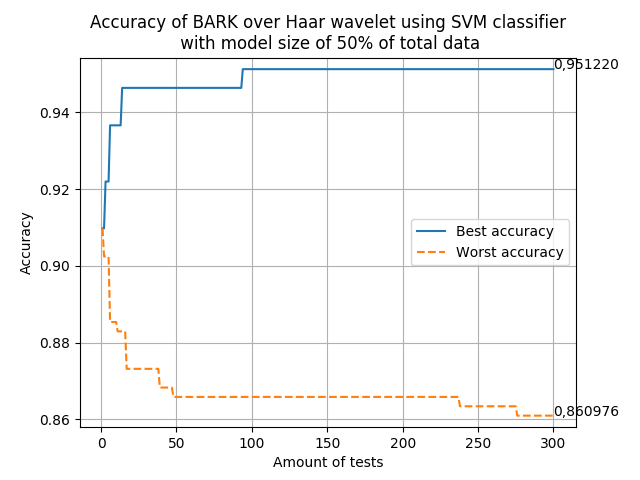
\includegraphics{images/results/confusionMatrices/classifier_SVM_50.png}
			\caption{Acurácia \textit{X} quantidade de testes - SVM, modelo a 50\%}
			\label{fig:classifiersvm50}
		\end{figure}
		\begin{table}[h] 					\newcommand{\mc}[3]{\multicolumn{#1}{#2}{#3}} 					\definecolor{tcB}{rgb}{0.447059,0.74902,0.266667} 					\definecolor{tcC}{rgb}{0,0,0} 					\definecolor{tcD}{rgb}{0,0.5,1} 					\definecolor{tcA}{rgb}{0.65098,0.65098,0.65098} 					\begin{center} 						\subfloat[Best confusion matrix]{ 							\begin{tabular}{ccc} 								\mc{1}{l}{} & \mc{1}{>{\columncolor{tcA}}c}{\textbf{genuine}} & \mc{1}{>{\columncolor{tcA}}c}{\textbf{spoofed}}\\ 								\mc{1}{>{\columncolor{tcA}}r}{\textbf{genuine}} & \mc{1}{>{\columncolor{tcB}}c}{\textcolor{tcC}{205}} & \mc{1}{>{\columncolor{tcD}}c}{\textcolor{tcC}{1}}\\ 								\mc{1}{>{\columncolor{tcA}}r}{\textbf{spoofed}} & \mc{1}{>{\columncolor{tcD}}c}{\textcolor{tcC}{0}} & \mc{1}{>{\columncolor{tcB}}c}{\textcolor{tcC}{204}} 							\end{tabular} 							\label{tab:classifier_SVM_50_best} 						} 						\qquad 						\subfloat[Worst confusion matrix]{ 							\begin{tabular}{ccc} 								\mc{1}{l}{} & \mc{1}{>{\columncolor{tcA}}c}{\textbf{genuine}} & \mc{1}{>{\columncolor{tcA}}c}{\textbf{spoofed}}\\ 								\mc{1}{>{\columncolor{tcA}}r}{\textbf{genuine}} & \mc{1}{>{\columncolor{tcB}}c}{\textcolor{tcC}{196}} & \mc{1}{>{\columncolor{tcD}}c}{\textcolor{tcC}{17}}\\ 								\mc{1}{>{\columncolor{tcA}}r}{\textbf{spoofed}} & \mc{1}{>{\columncolor{tcD}}c}{\textcolor{tcC}{9}} & \mc{1}{>{\columncolor{tcB}}c}{\textcolor{tcC}{188}} 							\end{tabular} 							\label{tab:classifier_SVM_50_worse} 						} 					\end{center} 					\caption{Confusion matrices for SVM distance classifier at 50\% model} 				\end{table}
	
	\newpage
	\section{Experimento 04}
		\par Os experimentos \ref{chap:propApproach:sec:Experimento01}, \ref{chap:propApproach:sec:Experimento02}, \ref{chap:propApproach:sec:Experimento03} mostraram que a combinação \textbf{\textit{wavelet haar + escala BARK}} é a melhor para geração de vetores de características e que esses possibilitam classificações razoáveis com classificadores simples. Esse experimento visa responder, qual o motivo dessa combinação funcionar melhor.
		\par As \textit{wavelets} \textbf{haar} e \textbf{daubechies 42} conseguiram respectivamente os melhores e os piores vetores de características na escala \textit{BARK}. Já em \textit{MEL}, \textbf{haar} foi a melhor e \textbf{daubechies 54} a pior.
		\par Para fins comparativos, foi criado um sinal periódico sobre o qual serão aplicadas as transformadas \textit{wavelet} correspondentes aos melhores e piores desempenhos, os resultados dessa aplicação, assim como o sinal original, constituem o gráfico mostrado na figura \ref{fig:haardaub42comparison}.
		\par O sinal periódico foi construído com a sequência \textit{32, 10, 20, 38, 37, 28, 38, 34, 18, 24, 24, 9, 23, 24, 28, 34} repetida 32 vezes.
		\par No gráfico supracitado o sinal de controle é periódico e contém 512 posições, portanto, considerando a abordagem de decomposição máxima, foram aplicadas as transformadas \textit{wavelet packet} até o nível 8.
		
		\begin{figure}[h]
			\centering
			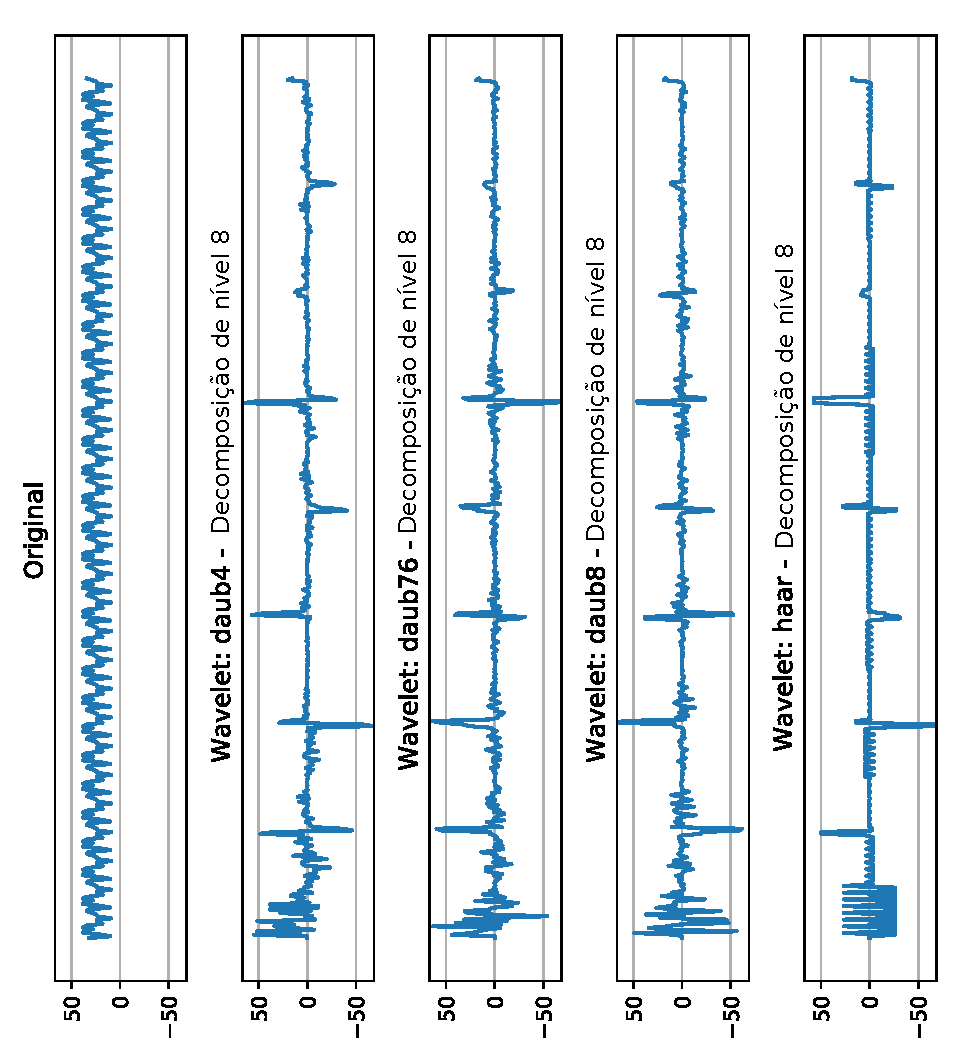
\includegraphics[width=0.6\linewidth]{images/results/haarDaubComparison/haarDaub42Comparison.pdf}
			\caption{Comparação wavelets \textit{haar} e \textit{daubechies 42, 54}}
			\label{fig:haardaub42comparison}
		\end{figure}
		
		\par É possível perceber que a separação das componentes do sinal é muito melhor delimitada na \textit{wavelet haar} do que na mesma transformação com a \textit{daubechies 42 e 54}, gerando assim um sinal mais separável, para ser lido tanto segundo a escala \textit{BARK} como \textit{MEL}.
		

	
	
	\chapter{Conclusões}
\label{chap:conclusions}
	\par As hipóteses iniciais neste trabalho consideravam que, a decomposição dos sinais ao máximo por \textit{wavelets} de qualquer natureza não alteraria o resultado quando do cálculo de energia do sinal segundo as escalas \textit{BARK} ou \textit{MEL} já que, no final, os intervalos das frequências seriam, de qualquer forma, tratados segundo as regras de cada escala.
	\par Após o exposto acima se mostrar falso, como constatado nos resultados (\ref{chap:testsResults:sec:Experimento01}) do experimento 1  (\ref{chap:propApproach:sec:Experimento01}) que demonstrou ser a combinação \textbf{\textit{wavelet packet haar + escala BARK} a melhor} posicionada no plano paraconsistente e \textit{wavelet packet daubeechies 54 + escala MEL} a pior, uma outra hipótese se formou após os resultado do experimento 2 e 3.
	\par A segunda hipótese formulada era que as combinações \textit{wavelet + BARK} eram superiores a \textit{wavelet + MEL}, pois a primeira cobria um intervalo de frequências um pouco maior. A ideia era que os ruídos adicionados no sinal por um gravador seriam de frequências, em boa parte, não presentes nas comunicações humanas e que, pela escala \textit{MEL} se basear na audição humana, esta seria inferior na detecção de interferências.
	\par Novamente, esse pensamento se provou incorreto. Analisando os gráficos (\ref{chap:testsResults:sec:Experimento05}) resultantes do experimento 5 (\ref{chap:propApproach:sec:Experimento05}), é possível notar que a escala \textbf{\textit{BARK} é superior a \textit{MEL} por considerar intervalos de frequências menores e em maior quantidade}, o que faz com que as diferenças das energias calculadas dentro da mesma classe (\textit{spoofing} ou \textit{não spoofing}) seja menor fazendo com que os vetores de características variem menos.
	\par No experimento 4 (\ref{chap:propApproach:sec:Experimento04}), não haviam hipóteses iniciais. Esta parte mostrou que a \textbf{transformada \textit{wavelet packet haar}, produz sinais com muito menos flutuações} que as outras wavelets usadas proporcionando uma melhor base para o cálculo das escalas \textit{BARK} e \textit{MEL}.
	\par Os experimentos 2 (\ref{chap:propApproach:sec:Experimento02}) e 3 (\ref{chap:propApproach:sec:Experimento03}) mostram nos seus respectivos resultados (\ref{chap:testsResults:sec:Experimento02} e \ref{chap:testsResults:sec:Experimento03}) que, \textbf{com ajuda da engenharia paraconsistente de características é possível fazer com que classificadores relativamente simples tenham desempenhos satisfatórios}.
	\par Por fim, \textbf{mestrado é difícil pra caramba!} Que venha o doutorado!
	
	\postextual
	
	\bibliography{bibliography.bib}
	
	\begin{apendicesenv}
	% Imprime uma página indicando o início dos apêndices
	\partapendices
	\begin{landscape}
		\chapter{Aplicação de um filtro \textit{Wavelet}}
		\begin{figure}[h]
			\caption{Demostração numérica das transformadas Wavelet e \textit{packet-wavelet}: Por razões didáticas a \textit{Wavelet} Haar foi considerada como tendo os valores $1/2$ e $-1/2$}
			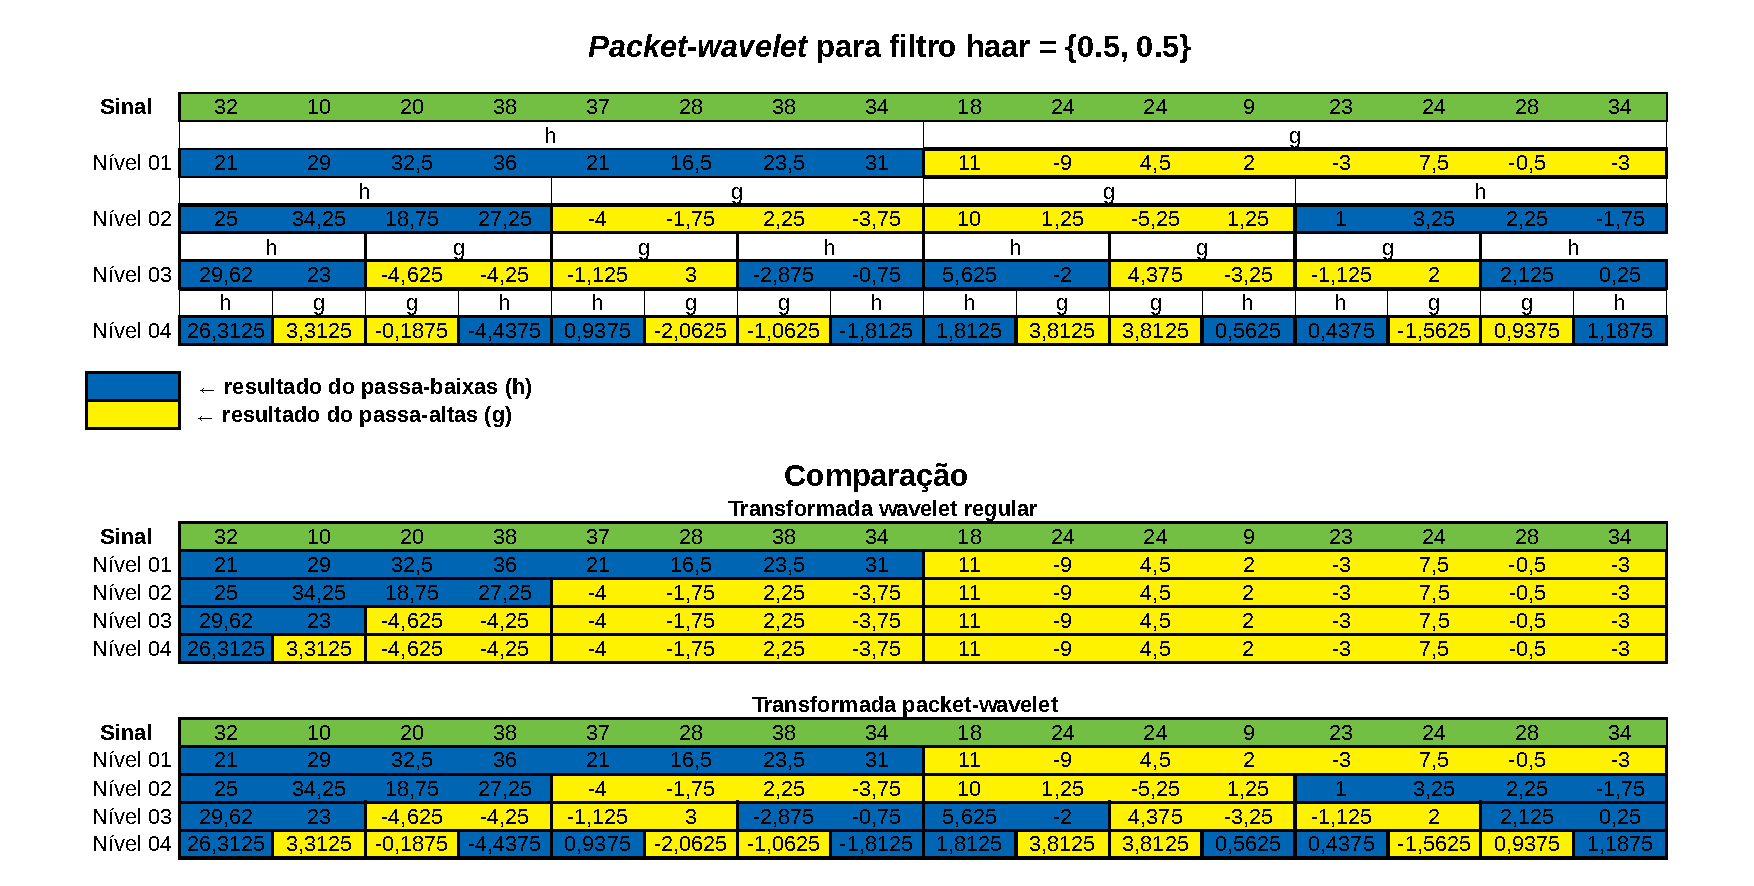
\includegraphics[width=.93\linewidth]{images/haarWaveletExamples.pdf}
			\label{fig:haarWaveletExamples}
			\\Fonte: Elaborado pelo autor, 2021.
			
		\end{figure}
	\end{landscape}

	\chapter{Arquivos digitais \textit{wave}}
		\label{chap:waveFile}
		\par Os arquivos no formato digital \textit{wave}, popularmente utilizados para armazenar áudio e voz digital \cite{WAVE2019}, assim como ocorre neste trabalho, se estruturam como ilustrado na Figura \ref{fig:wavePcmStructure}.
		
		\begin{figure}[h]
			\centering
			\caption{Estrutura do arquivo Wave}
			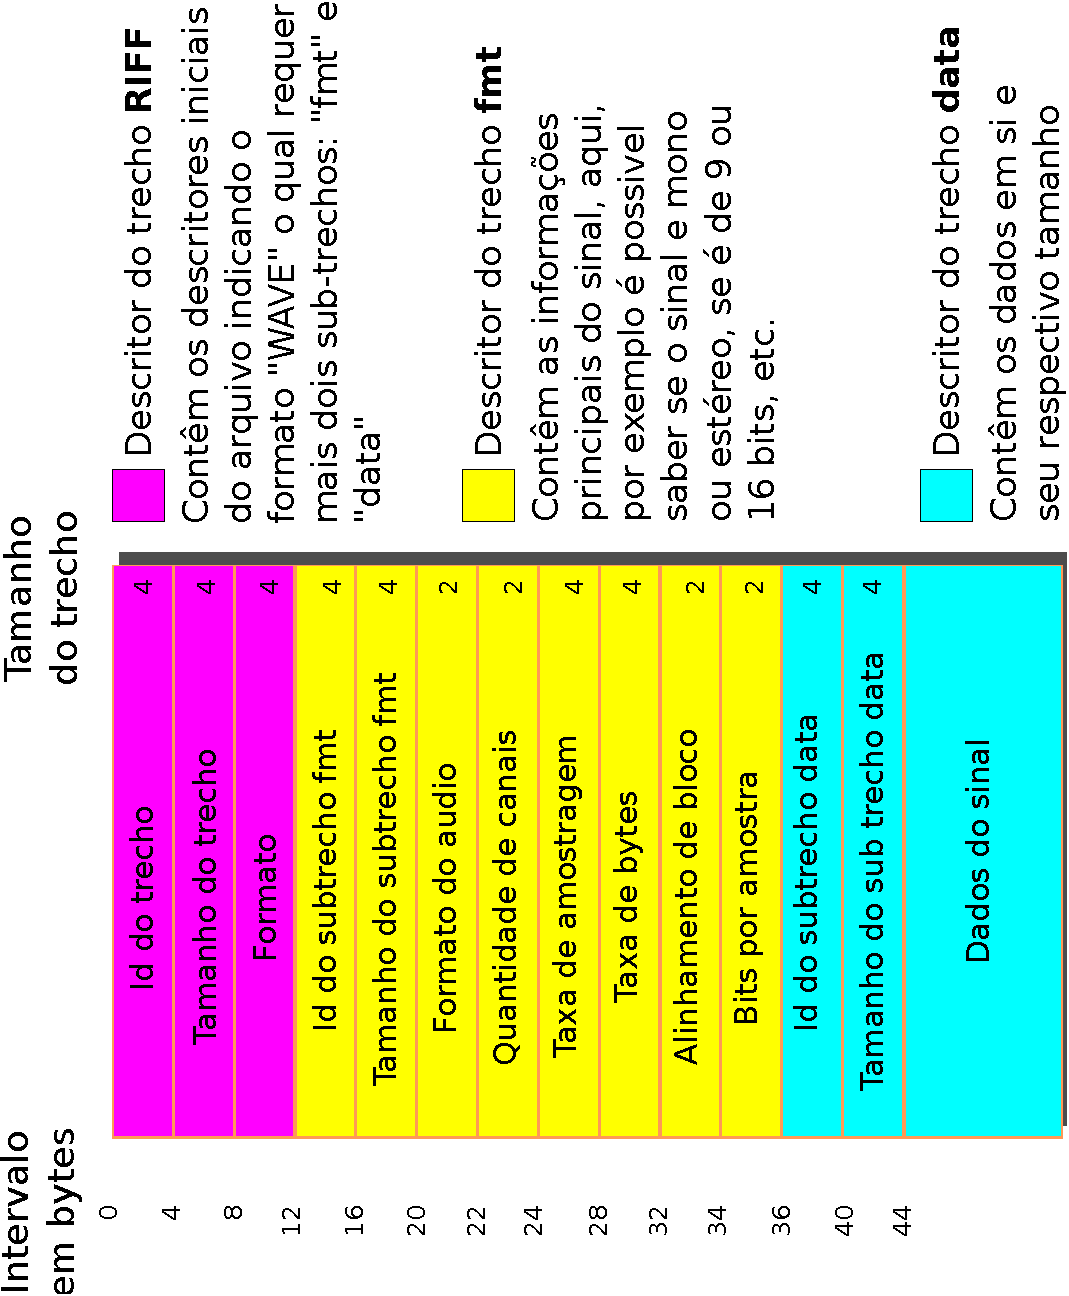
\includegraphics[width=0.6\linewidth, angle=-90]{images/wavePcmStructure.pdf}
			\label{fig:wavePcmStructure}
			\\Fonte: Elaborado pelo autor, 2021.
		\end{figure}
		
		\par A estrutura de interesse se localiza na última parte do arquivo, mais especificamente no bloco ``data'' ilustrado em azul na Figura. Nele, os dados são organizados como um grande vetor de números, em formato \textit{little endian} \cite{adiga2007writing}, sendo que cada um deles indica a intensidade do sinal naquele ponto. A descrição pormenorizada do bloco ``data'', consultada em \cite{microsoftIbmWaveSpec}, foi utilizada neste trabalho para possibilitar a extração dos dados brutos dos sinais utilizados. 

	\chapter{Recursos na web}
		\par Para realização deste trabalho foram produzidos variados textos (este incluso) e códigos, é recomendada a consulta dos códigos fontes utilizados nos procedimentos como complemento que, se espera, melhore o entendimento dos assuntos discutidos.
		
		\par Uma atenção especial deve ser dada ao diretório localizado em \textit{\textbf{/src/lib}} que contém todas as bibliotecas criadas e referenciadas para resolver os problemas surgidos e também ao \textit{\textbf{/src/experiments}} que contém os procedimentos já descritos.
				
		\par Em \textit{\textbf{/soundSamples}} se encontra a base de dados com os áudios originais e tratados.
		
		\par Alguns \textit{scripts} foram desenvolvidos para facilitar o tratamento dos arquivos de áudio, os mesmos se encontram em \textbf{\textit{/src/scripts}}.
		
		\par Por fim a parte escrita pode ser consultada em \textit{\textbf{/documentation}}.
		
		\par Todos esses materiais estão sob licença de código aberto (GPLv3) e são livres para uso não comercial acesse   \href{https://github.com/ensismoebius/voiceSpoofingDetectionWavelet}{https://github.com/ensismoebius/voiceSpoofingDetectionWavelet} para mais informações.
\end{apendicesenv}

	\phantompart
	\printindex
\end{document}




